\documentclass[ignorenonframetext,]{beamer}
\setbeamertemplate{caption}[numbered]
\setbeamertemplate{caption label separator}{: }
\setbeamercolor{caption name}{fg=normal text.fg}
\beamertemplatenavigationsymbolsempty
\usepackage{lmodern}
\usepackage{amssymb,amsmath}
\usepackage{ifxetex,ifluatex}
\usepackage{fixltx2e} % provides \textsubscript
\ifnum 0\ifxetex 1\fi\ifluatex 1\fi=0 % if pdftex
  \usepackage[T1]{fontenc}
  \usepackage[utf8]{inputenc}
\else % if luatex or xelatex
  \ifxetex
    \usepackage{mathspec}
  \else
    \usepackage{fontspec}
  \fi
  \defaultfontfeatures{Ligatures=TeX,Scale=MatchLowercase}
\fi
% use upquote if available, for straight quotes in verbatim environments
\IfFileExists{upquote.sty}{\usepackage{upquote}}{}
% use microtype if available
\IfFileExists{microtype.sty}{%
\usepackage{microtype}
\UseMicrotypeSet[protrusion]{basicmath} % disable protrusion for tt fonts
}{}
\newif\ifbibliography
\hypersetup{
            pdftitle={Random Effects ANCOVA},
            pdfborder={0 0 0},
            breaklinks=true}
\urlstyle{same}  % don't use monospace font for urls
\usepackage{color}
\usepackage{fancyvrb}
\newcommand{\VerbBar}{|}
\newcommand{\VERB}{\Verb[commandchars=\\\{\}]}
\DefineVerbatimEnvironment{Highlighting}{Verbatim}{commandchars=\\\{\}}
% Add ',fontsize=\small' for more characters per line
\usepackage{framed}
\definecolor{shadecolor}{RGB}{248,248,248}
\newenvironment{Shaded}{\begin{snugshade}}{\end{snugshade}}
\newcommand{\KeywordTok}[1]{\textcolor[rgb]{0.13,0.29,0.53}{\textbf{#1}}}
\newcommand{\DataTypeTok}[1]{\textcolor[rgb]{0.13,0.29,0.53}{#1}}
\newcommand{\DecValTok}[1]{\textcolor[rgb]{0.00,0.00,0.81}{#1}}
\newcommand{\BaseNTok}[1]{\textcolor[rgb]{0.00,0.00,0.81}{#1}}
\newcommand{\FloatTok}[1]{\textcolor[rgb]{0.00,0.00,0.81}{#1}}
\newcommand{\ConstantTok}[1]{\textcolor[rgb]{0.00,0.00,0.00}{#1}}
\newcommand{\CharTok}[1]{\textcolor[rgb]{0.31,0.60,0.02}{#1}}
\newcommand{\SpecialCharTok}[1]{\textcolor[rgb]{0.00,0.00,0.00}{#1}}
\newcommand{\StringTok}[1]{\textcolor[rgb]{0.31,0.60,0.02}{#1}}
\newcommand{\VerbatimStringTok}[1]{\textcolor[rgb]{0.31,0.60,0.02}{#1}}
\newcommand{\SpecialStringTok}[1]{\textcolor[rgb]{0.31,0.60,0.02}{#1}}
\newcommand{\ImportTok}[1]{#1}
\newcommand{\CommentTok}[1]{\textcolor[rgb]{0.56,0.35,0.01}{\textit{#1}}}
\newcommand{\DocumentationTok}[1]{\textcolor[rgb]{0.56,0.35,0.01}{\textbf{\textit{#1}}}}
\newcommand{\AnnotationTok}[1]{\textcolor[rgb]{0.56,0.35,0.01}{\textbf{\textit{#1}}}}
\newcommand{\CommentVarTok}[1]{\textcolor[rgb]{0.56,0.35,0.01}{\textbf{\textit{#1}}}}
\newcommand{\OtherTok}[1]{\textcolor[rgb]{0.56,0.35,0.01}{#1}}
\newcommand{\FunctionTok}[1]{\textcolor[rgb]{0.00,0.00,0.00}{#1}}
\newcommand{\VariableTok}[1]{\textcolor[rgb]{0.00,0.00,0.00}{#1}}
\newcommand{\ControlFlowTok}[1]{\textcolor[rgb]{0.13,0.29,0.53}{\textbf{#1}}}
\newcommand{\OperatorTok}[1]{\textcolor[rgb]{0.81,0.36,0.00}{\textbf{#1}}}
\newcommand{\BuiltInTok}[1]{#1}
\newcommand{\ExtensionTok}[1]{#1}
\newcommand{\PreprocessorTok}[1]{\textcolor[rgb]{0.56,0.35,0.01}{\textit{#1}}}
\newcommand{\AttributeTok}[1]{\textcolor[rgb]{0.77,0.63,0.00}{#1}}
\newcommand{\RegionMarkerTok}[1]{#1}
\newcommand{\InformationTok}[1]{\textcolor[rgb]{0.56,0.35,0.01}{\textbf{\textit{#1}}}}
\newcommand{\WarningTok}[1]{\textcolor[rgb]{0.56,0.35,0.01}{\textbf{\textit{#1}}}}
\newcommand{\AlertTok}[1]{\textcolor[rgb]{0.94,0.16,0.16}{#1}}
\newcommand{\ErrorTok}[1]{\textcolor[rgb]{0.64,0.00,0.00}{\textbf{#1}}}
\newcommand{\NormalTok}[1]{#1}
\usepackage{graphicx,grffile}
\makeatletter
\def\maxwidth{\ifdim\Gin@nat@width>\linewidth\linewidth\else\Gin@nat@width\fi}
\def\maxheight{\ifdim\Gin@nat@height>\textheight0.8\textheight\else\Gin@nat@height\fi}
\makeatother
% Scale images if necessary, so that they will not overflow the page
% margins by default, and it is still possible to overwrite the defaults
% using explicit options in \includegraphics[width, height, ...]{}
\setkeys{Gin}{width=\maxwidth,height=\maxheight,keepaspectratio}

% Prevent slide breaks in the middle of a paragraph:
\widowpenalties 1 10000
\raggedbottom

\AtBeginPart{
  \let\insertpartnumber\relax
  \let\partname\relax
  \frame{\partpage}
}
\AtBeginSection{
  \ifbibliography
  \else
    \let\insertsectionnumber\relax
    \let\sectionname\relax
    \frame{\sectionpage}
  \fi
}
\AtBeginSubsection{
  \let\insertsubsectionnumber\relax
  \let\subsectionname\relax
  \frame{\subsectionpage}
}

\setlength{\parindent}{0pt}
\setlength{\parskip}{6pt plus 2pt minus 1pt}
\setlength{\emergencystretch}{3em}  % prevent overfull lines
\providecommand{\tightlist}{%
  \setlength{\itemsep}{0pt}\setlength{\parskip}{0pt}}
\setcounter{secnumdepth}{0}

\title{Random Effects ANCOVA}
\date{}

\begin{document}
\frame{\titlepage}

\begin{frame}{Reading}

This set of notes is based on Hoff Chapter 5.

\end{frame}

\begin{frame}{ANCOVA}

\begin{quote}
``What's in a name? That which we call a rose\\
By any other name would smell as sweet.''

\hfill --- Romeo and Juliet II, ii, 1-2
\end{quote}

\begin{figure}
\centering
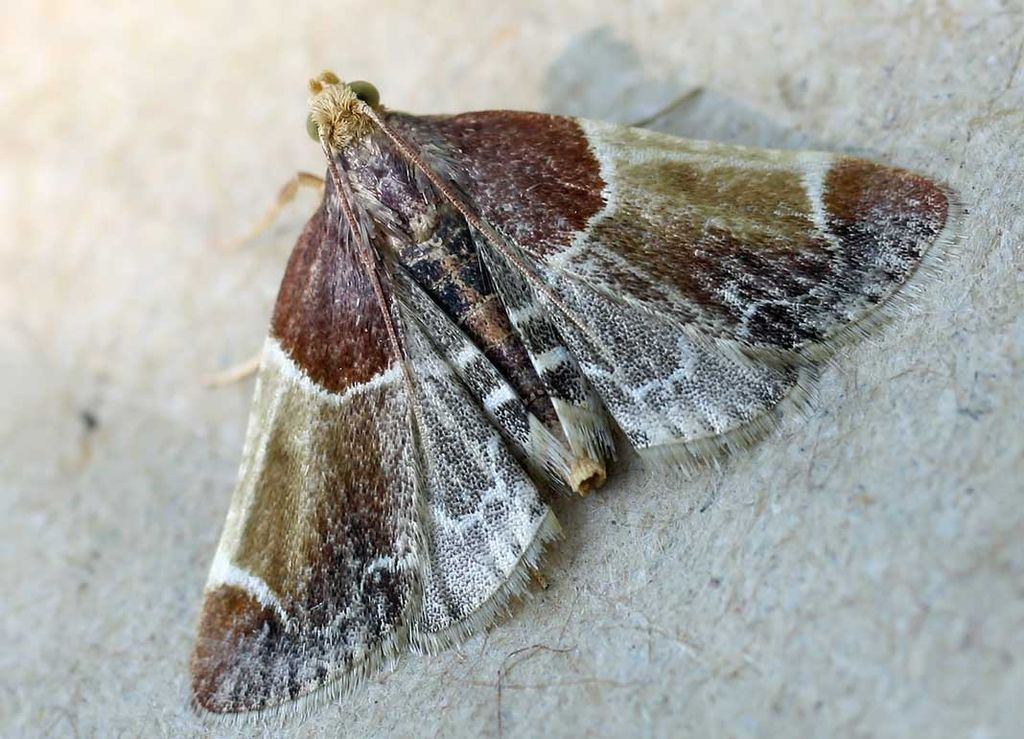
\includegraphics[width=0.40000\textwidth]{figures/ancovamoth.jpg}
\caption{Ancova moth, or snout moth}
\end{figure}

ANOVA, ANCOVA, MANOVA -- what's the difference?

\end{frame}

\begin{frame}{}

\begin{itemize}
\item
  ANOVA (Analysis of Variance): continuous outcome, categorical
  predictor(s)

  \begin{itemize}
  \tightlist
  \item
    one-way ANOVA: one categorical predictor
  \item
    two-way ANOVA: two categorical predictors
  \item
    two-way ANOVA with interaction: you get the picture!
  \end{itemize}
\item
  ANCOVA (Analysis of Covariance): continuous outcome, categorical
  predictor(s), at least one continuous predictor that is generally
  considered a nuisance (not unlike the snout moths, which are often
  considered pests because they share our tastes in grains)
\item
  MANOVA (Multivariate ANOVA): multiple continuous outcomes, categorical
  predictor(s)
\end{itemize}

Historically these names had implications regarding the estimation
methods used, but that is no longer always the case.

\end{frame}

\begin{frame}{Motivating Example: National Educational Longitudinal
Study of Education (NELS)}

Hoff considers a subset of the NELS data that contains information on
math scores of a random sample of 10th graders selected from a national
sample of 100 large urban public schools. We plot the math scores
\(y_{ij}\) of the \(n_j\) students in each school \(j\), ranked by the
average score.

\end{frame}

\begin{frame}{}

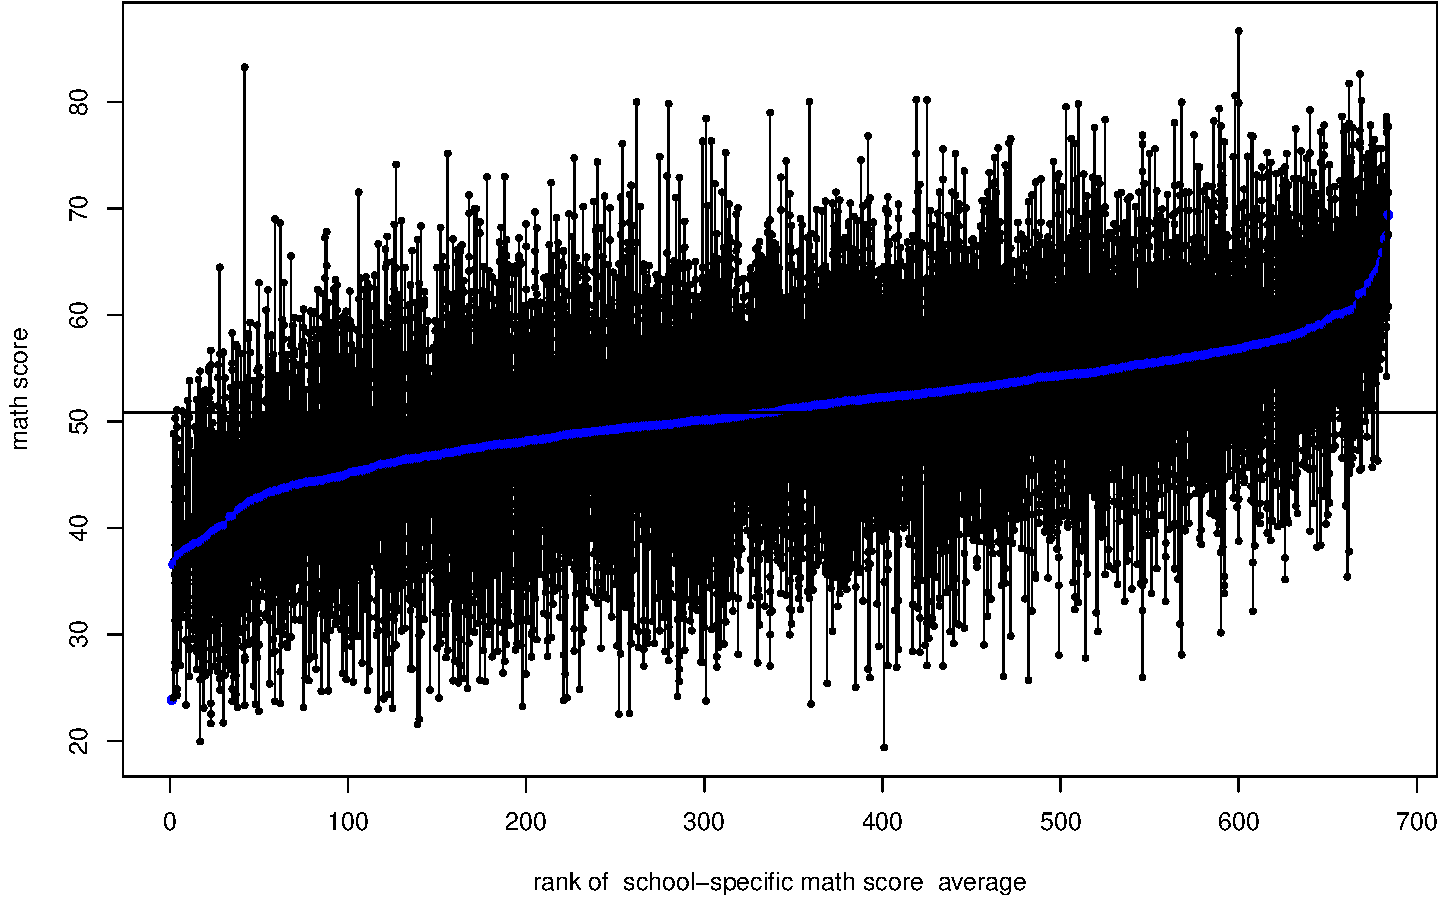
\includegraphics{ancova_01_deck_files/figure-beamer/nelsplot1-1.pdf}

\end{frame}

\begin{frame}{}

\begin{itemize}
\item
  The school-specific averages range from 36.58 to 65.02, with 48.13 the
  average of all 100 school averages (weighting each school equally).
\item
  The school-specific variances range from 21.81 to 179.69 -- quite a
  wide range!
\item
  The school with the highest average only contains 4 observations.
\end{itemize}

\end{frame}

\begin{frame}{Which school is best?}

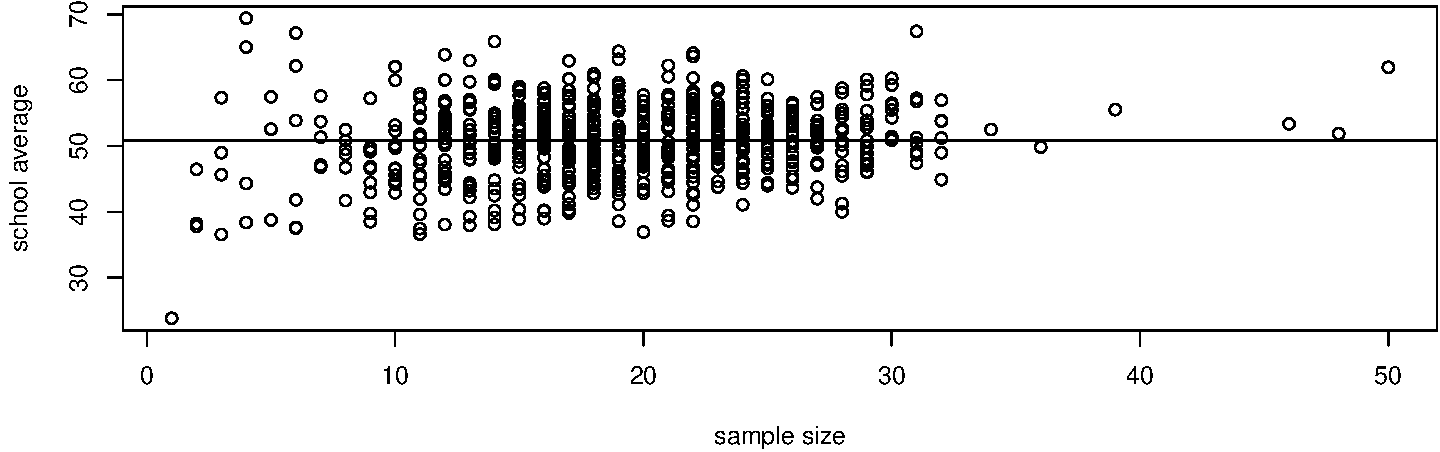
\includegraphics{ancova_01_deck_files/figure-beamer/nelsplot2-1.pdf}

Note that the school with the highest average has the smallest sample
size (\(n_j=4\)). Do we have strong evidence that the true mean in this
school is substantially larger than that in other schools in the sample?
How might we answer this question?

\end{frame}

\begin{frame}[fragile]{ANOVA}

One approach would be to fit a fixed effects ANOVA model:

\begin{Shaded}
\begin{Highlighting}[]
\NormalTok{m1=}\KeywordTok{lm}\NormalTok{(nels_mathdat}\OperatorTok{$}\NormalTok{mscore}\OperatorTok{~}\KeywordTok{as.factor}\NormalTok{(nels_mathdat}\OperatorTok{$}\NormalTok{school)}\OperatorTok{-}\DecValTok{1}\NormalTok{)}
\KeywordTok{anova}\NormalTok{(m1)}
\end{Highlighting}
\end{Shaded}

\begin{verbatim}
## Analysis of Variance Table
## 
## Response: nels_mathdat$mscore
##                                   Df   Sum Sq Mean Sq F value    Pr(>F)
## as.factor(nels_mathdat$school)   684 34306852   50156  681.54 < 2.2e-16
## Residuals                      12290   904450      74                  
##                                   
## as.factor(nels_mathdat$school) ***
## Residuals                         
## ---
## Signif. codes:  0 '***' 0.001 '**' 0.01 '*' 0.05 '.' 0.1 ' ' 1
\end{verbatim}

Here we see clear evidence of heterogeneity in math scores across
schools.

\end{frame}

\begin{frame}[fragile]{ANOVA results}

\begin{Shaded}
\begin{Highlighting}[]
\KeywordTok{library}\NormalTok{(sjPlot)}
\KeywordTok{plot_model}\NormalTok{(m1,}\DataTypeTok{sort.est=}\OtherTok{TRUE}\NormalTok{)}
\end{Highlighting}
\end{Shaded}

\end{frame}

\begin{frame}{}

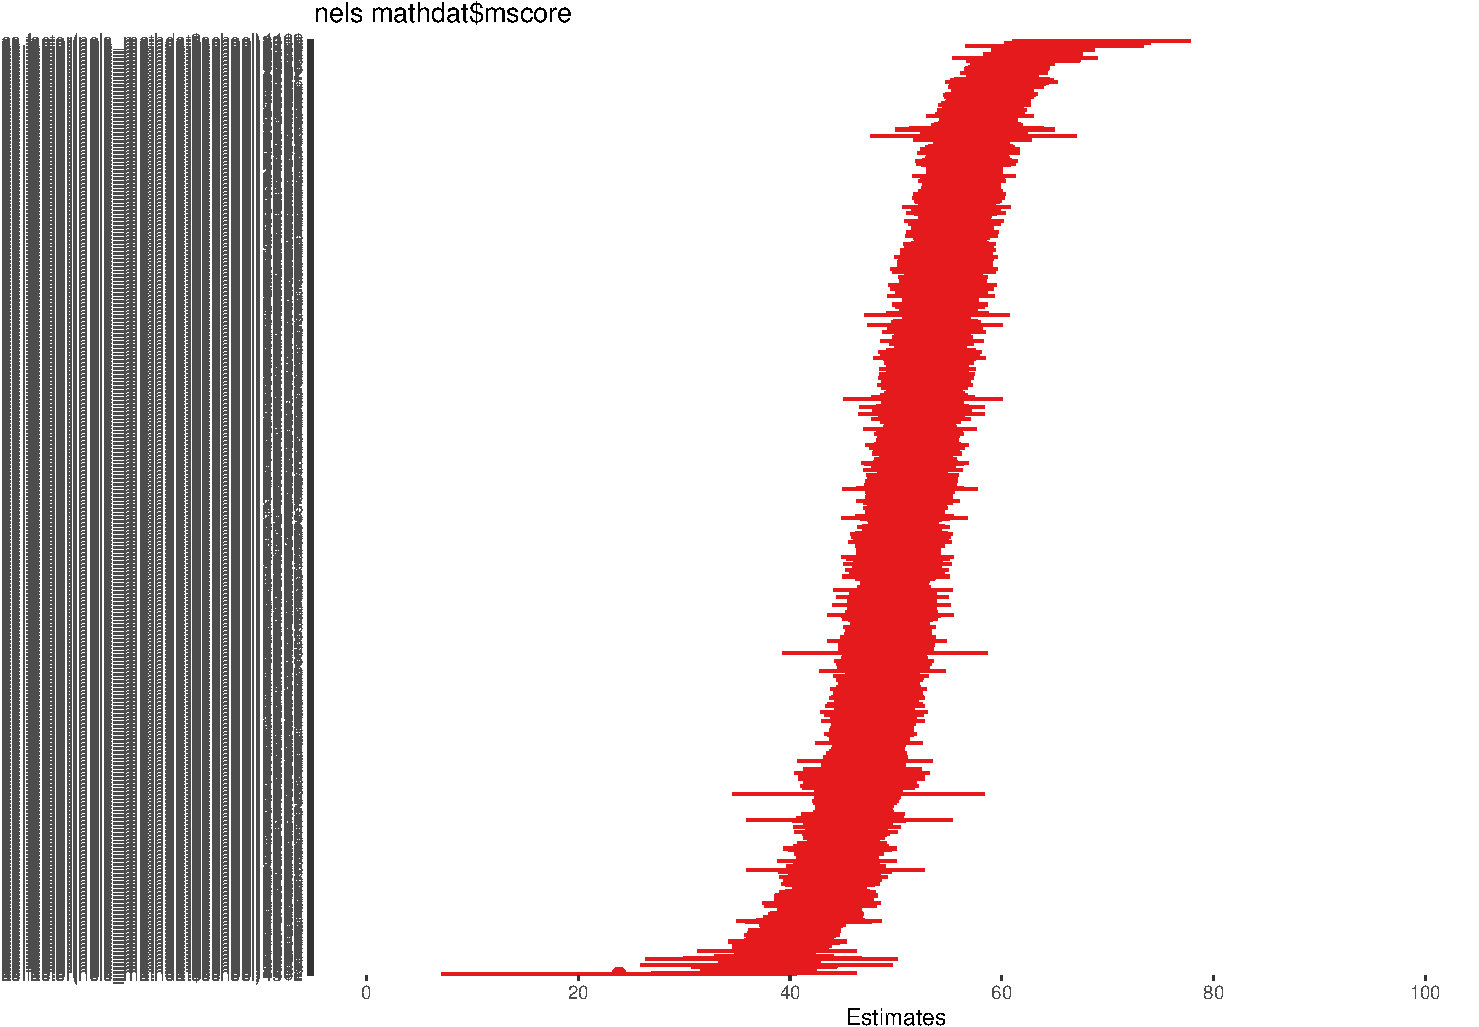
\includegraphics{ancova_01_deck_files/figure-beamer/catplot1-1.pdf}

Based on these estimates, we might conclude that the school has higher
performance than some, but not all, schools.

\end{frame}

\begin{frame}[fragile]{Random effects ANOVA}

Note in the prior plot that the highest estimated mean also has a very
large variance. We may wish to use shrinkage estimation in order to
stabilize that and other estimates for schools in which few students
provide data. A random effects ANOVA model is given by
\[y_{ij}=\mu+\alpha_j+\varepsilon_{ij},\] where
\(\varepsilon_{ij} \sim N(0,\sigma^2)\) and
\(\alpha_j \sim N(0,\tau^2)\).

\begin{Shaded}
\begin{Highlighting}[]
\KeywordTok{library}\NormalTok{(lme4)}
\NormalTok{m2=}\KeywordTok{lmer}\NormalTok{(mscore}\OperatorTok{~}\NormalTok{(}\DecValTok{1}\OperatorTok{|}\NormalTok{school),}\DataTypeTok{data=}\NormalTok{nels_mathdat)}
\KeywordTok{summary}\NormalTok{(m2)}
\KeywordTok{library}\NormalTok{(sjstats)}
\KeywordTok{icc}\NormalTok{(m2)}
\end{Highlighting}
\end{Shaded}

\end{frame}

\begin{frame}[fragile]{}

\begin{verbatim}
## Linear mixed model fit by REML ['lmerMod']
## Formula: mscore ~ (1 | school)
##    Data: nels_mathdat
## 
## REML criterion at convergence: 93914.6
## 
## Scaled residuals: 
##     Min      1Q  Median      3Q     Max 
## -3.8113 -0.6534  0.0094  0.6732  4.7000 
## 
## Random effects:
##  Groups   Name        Variance Std.Dev.
##  school   (Intercept) 23.68    4.866   
##  Residual             73.71    8.585   
## Number of obs: 12974, groups:  school, 684
## 
## Fixed effects:
##             Estimate Std. Error t value
## (Intercept)  50.9390     0.2028   251.2
\end{verbatim}

\begin{verbatim}
## # Intraclass Correlation Coefficient
## 
##      Adjusted ICC: 0.243
##   Conditional ICC: 0.243
\end{verbatim}

\end{frame}

\begin{frame}[fragile]{}

Here we examine the distribution of random effects.

\begin{Shaded}
\begin{Highlighting}[]
\KeywordTok{library}\NormalTok{(merTools)}
\KeywordTok{plotREsim}\NormalTok{(}\KeywordTok{REsim}\NormalTok{(m2,}\DataTypeTok{n.sims=}\DecValTok{100}\NormalTok{),}\DataTypeTok{stat=}\StringTok{'median'}\NormalTok{,}\DataTypeTok{sd=}\OtherTok{TRUE}\NormalTok{)}
\end{Highlighting}
\end{Shaded}

\end{frame}

\begin{frame}{}

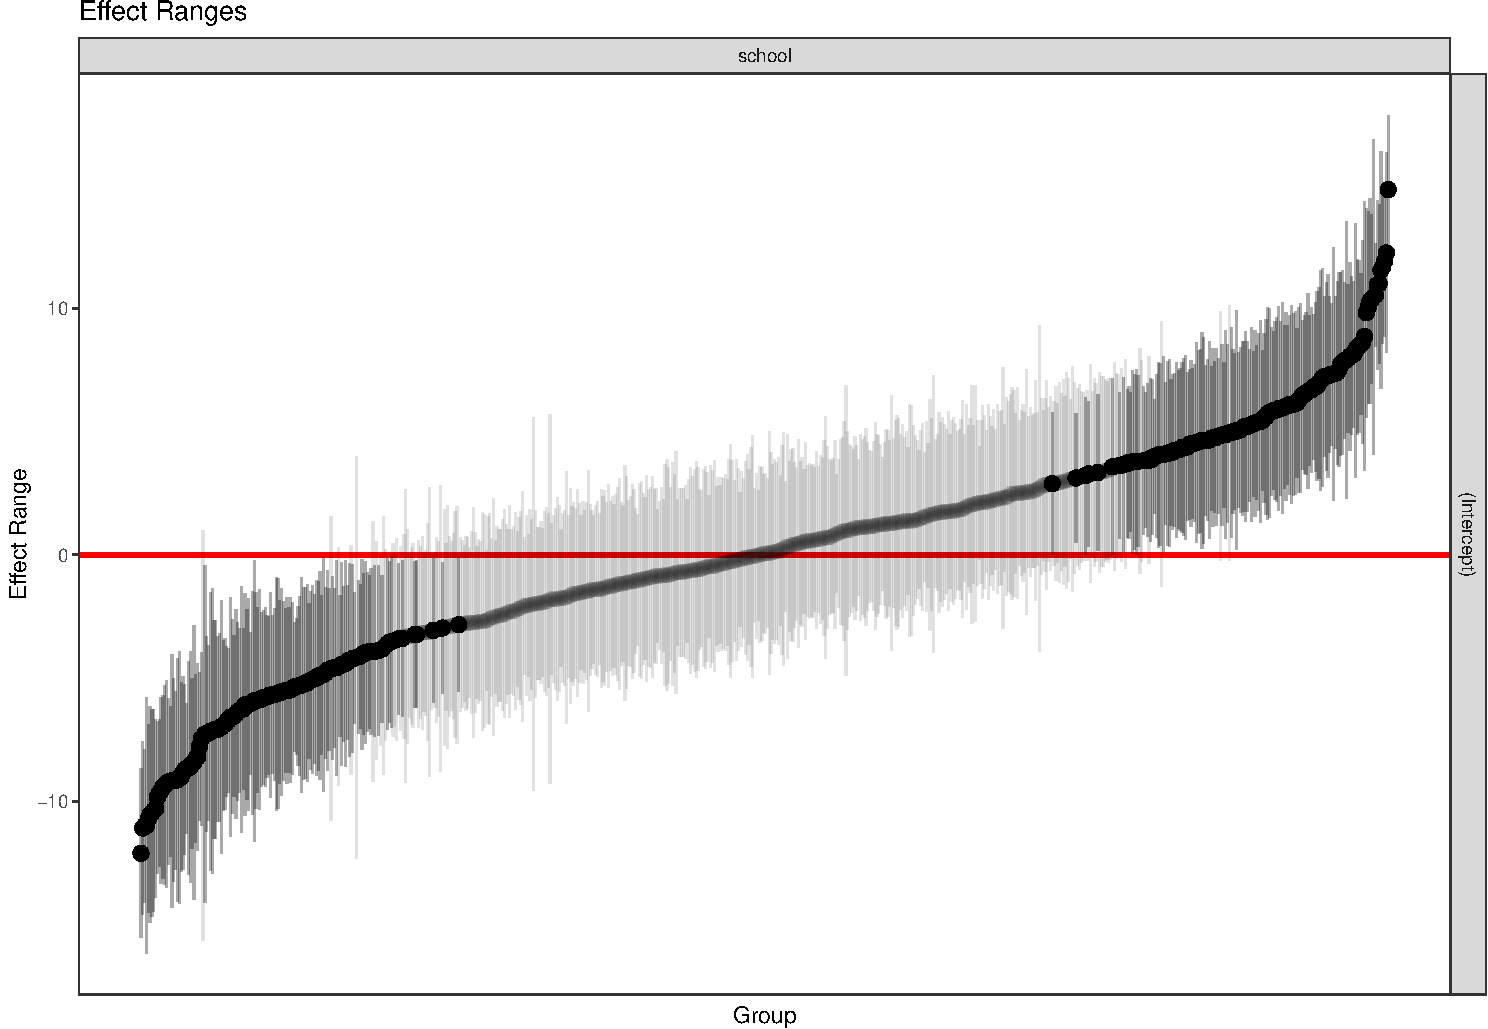
\includegraphics{ancova_01_deck_files/figure-beamer/plotre2-1.pdf}

\end{frame}

\begin{frame}{}

How do we conduct a formal test of heterogeneity in this random effects
setting? Well, this is a bit more complicated than in the fixed effects
setting. In particular, no heterogeneity corresponds to the case in
which \(\tau^2=0 \iff \alpha_1=\ldots=\alpha_J=0\), so saying something
about the single parameter \(\tau^2\) has implications about the J
parameters \(\alpha_j\).

A second problem is that \(\tau^2\) cannot be \(<0\), and we wish to
test \(H_0: \tau^2=0\), so we're conducting a hypothesis test at the
boundary of the parameter space instead of in the interior (which would
be the case for \(H_0: \mu=0\)).

\end{frame}

\begin{frame}{}

As shown in Stram and Lee (1994), the approximate asymptotic null
distribution for \(H_0: \tau^2=0\) using a likelihood ratio test
comparing our model to a model with out random effects
(\(y_{ij}=\mu+\varepsilon_{ij}\)) in this case is a 50-50 mixture of a
\(\chi^2_0\) (point mass on 0) and a \(\chi_1^2\) distribution.

\end{frame}

\begin{frame}{}

In general, if we wish to compare a model with \(q+1\) random effects
(calculated as terms that have a random effect, not the number of
groups) to a nested model with \(q\) random effects, the asymptotic null
distribution is a 50-50 mixture of \(\chi^2_{q+1}\) and \(\chi^2_q\)
distributions.

\end{frame}

\begin{frame}{}

Letting LR denote twice the difference in maximized log-likelihoods in
the model with and without a single random effect, you can obtain the
null density in R using
\[0.5*(\text{dchisq}(x,q+1)+\text{dchisq}(x,q))\] and the p-value via
\[0.5*(1-\text{pchisq(LR,q+1)}+1-\text{pchisq}(LR,q)).\]

\end{frame}

\begin{frame}[fragile]{}

For the NELS data fit using a frequentist random effects model, we would
calculate this as follows.

\begin{Shaded}
\begin{Highlighting}[]
\NormalTok{m3=}\KeywordTok{lmer}\NormalTok{(mscore}\OperatorTok{~}\NormalTok{(}\DecValTok{1}\OperatorTok{|}\NormalTok{school),}\DataTypeTok{data=}\NormalTok{nels_mathdat,}\DataTypeTok{REML=}\OtherTok{FALSE}\NormalTok{)}
\NormalTok{m4=}\KeywordTok{lm}\NormalTok{(mscore}\OperatorTok{~}\DecValTok{1}\NormalTok{,}\DataTypeTok{data=}\NormalTok{nels_mathdat)}
\NormalTok{LR=}\KeywordTok{logLik}\NormalTok{(m3)}\OperatorTok{-}\KeywordTok{logLik}\NormalTok{(m4)}
\FloatTok{0.5}\OperatorTok{*}\NormalTok{(}\DecValTok{1}\OperatorTok{-}\KeywordTok{pchisq}\NormalTok{(LR[}\DecValTok{1}\NormalTok{],}\DecValTok{1}\NormalTok{)}\OperatorTok{+}\DecValTok{1}\OperatorTok{-}\KeywordTok{pchisq}\NormalTok{(LR[}\DecValTok{1}\NormalTok{],}\DecValTok{0}\NormalTok{))}
\end{Highlighting}
\end{Shaded}

\begin{verbatim}
## [1] 0
\end{verbatim}

We conclude that there is significant heterogeneity across schools in
the mean math scores.

\end{frame}

\begin{frame}{Bringing SES into the mix}

NELS contains a measure of socioeconomic status (SES) for each student.
We generally expect some degree of correlation between SES and math
score (people who are good at math often can get good jobs, and then
have kids who may inherit math talents; rich parents may have more time
and resources to devote to their kids), though of course the
relationship is not deterministic (there are plenty of math whizzes who
did not have rich parents -- Gauss!, and there are plenty of rich
parents who have kids who do not make good math scores -- college
admissions scandal!).

\end{frame}

\begin{frame}{}

Let's look overall at the association between SES and math score in
NELS.

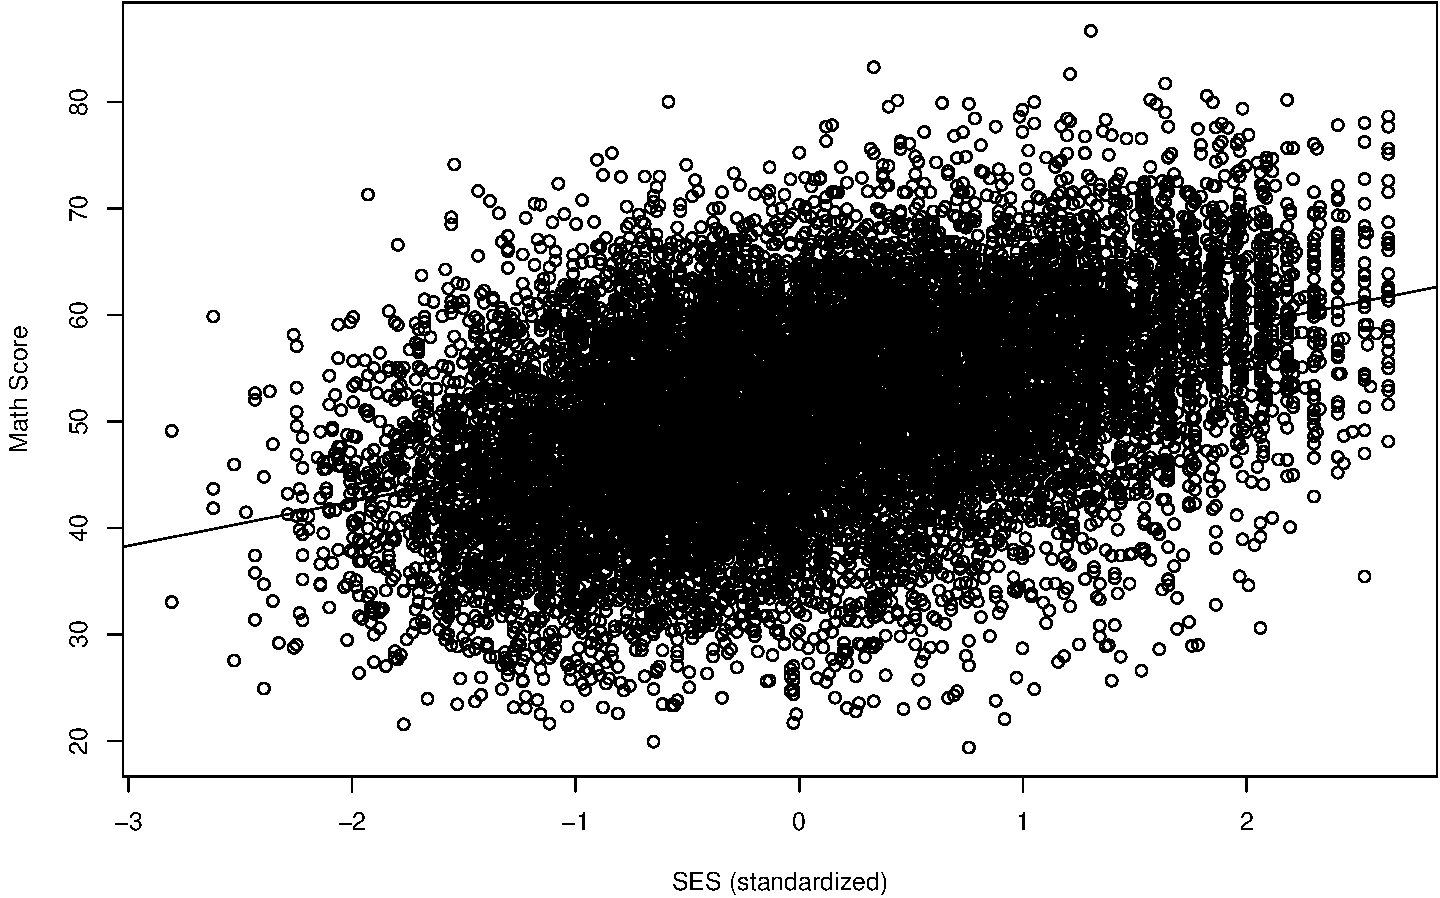
\includegraphics[width=0.8\linewidth]{ancova_01_deck_files/figure-beamer/scatter-1}

\end{frame}

\begin{frame}{Big Picture}

Consider schools, which we represent using red, green, and blue points
on graphs, respectively. The schools we illustrate include one low SES
school, one middle SES school, and one high SES school.

Let's consider multiple ways in which we could obtain the marginal
association between SES and math score on the previous slide.

\end{frame}

\begin{frame}{}

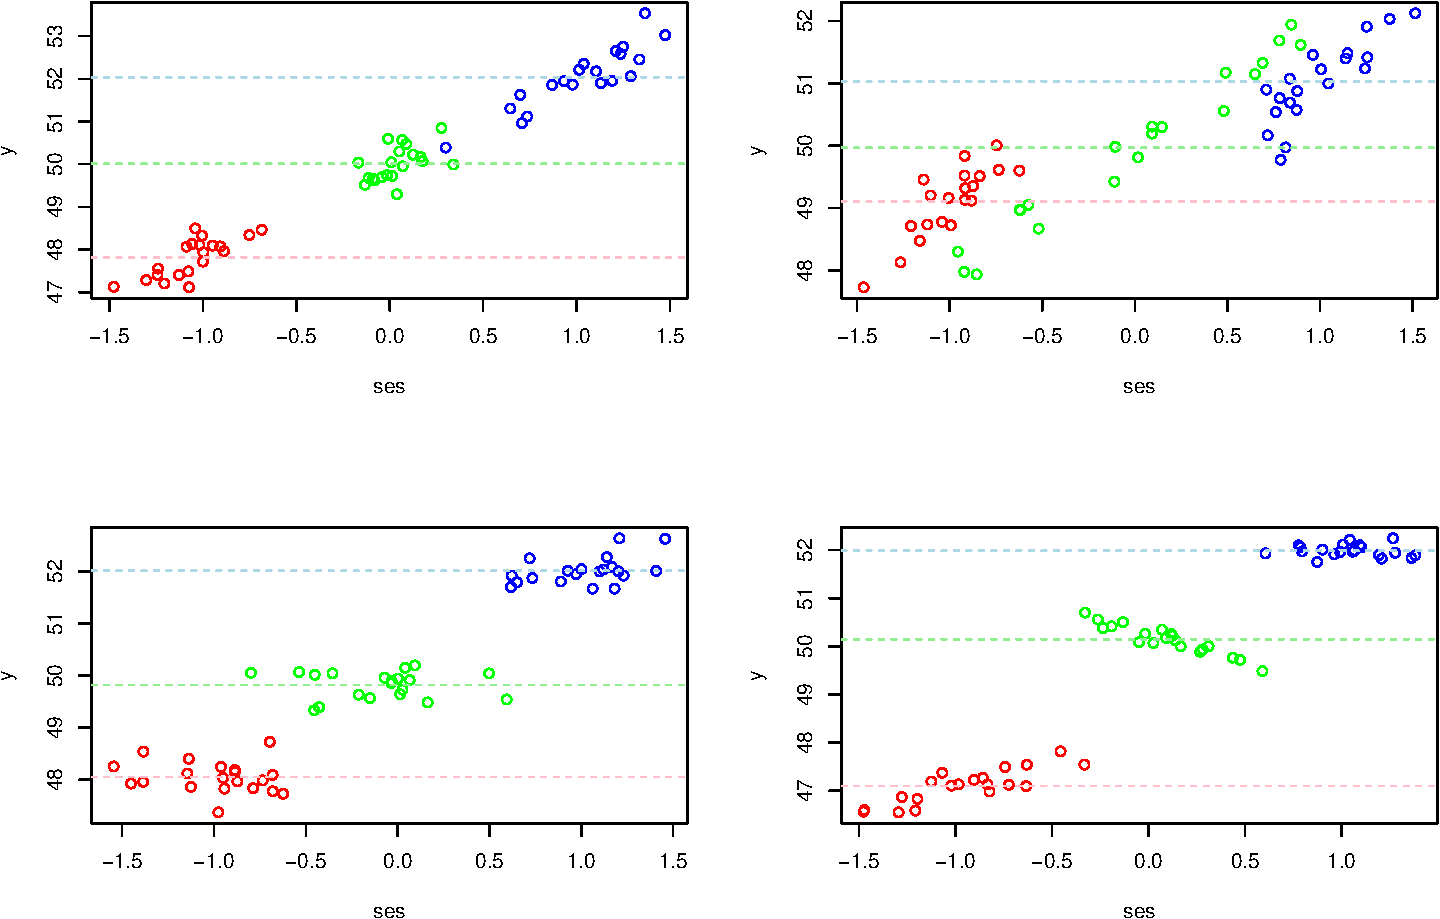
\includegraphics[width=0.6\linewidth]{ancova_01_deck_files/figure-beamer/illustrateplot-1}

We want our model to be able to help us understand how SES (\(x_{ij}\))
and math scores are related in schools. In the framework of the model
\(y_{ij}=\beta_{0,j}+\beta_{1,j}x_{ij} + \varepsilon_{ij}\), what values
of \(\beta_{j}\) are consistent with these figures?

\end{frame}

\begin{frame}{}

One way to assess how SES is related to math score is to examine this
association in an ANCOVA model, allowing school-specific intercepts
while including SES as a covariate \(x_{ij}\):

\[y_{ij}=\beta_{0j}+\beta_1x_{ij} + \varepsilon_{ij}.\]

In this model, we estimate the same effect of SES for each school.

\end{frame}

\begin{frame}[fragile]{}

\begin{Shaded}
\begin{Highlighting}[]
\NormalTok{m5=}\KeywordTok{lmer}\NormalTok{(mscore}\OperatorTok{~}\NormalTok{sesstd}\OperatorTok{+}\NormalTok{(}\DecValTok{1}\OperatorTok{|}\NormalTok{school),}\DataTypeTok{data=}\NormalTok{nels_mathdat)}
\KeywordTok{summary}\NormalTok{(m5)}
\end{Highlighting}
\end{Shaded}

\begin{verbatim}
## Linear mixed model fit by REML ['lmerMod']
## Formula: mscore ~ sesstd + (1 | school)
##    Data: nels_mathdat
## 
## REML criterion at convergence: 92558.7
## 
## Scaled residuals: 
##     Min      1Q  Median      3Q     Max 
## -3.8753 -0.6428  0.0165  0.6693  4.4322 
## 
## Random effects:
##  Groups   Name        Variance Std.Dev.
##  school   (Intercept) 12.22    3.495   
##  Residual             68.03    8.248   
## Number of obs: 12974, groups:  school, 684
## 
## Fixed effects:
##             Estimate Std. Error t value
## (Intercept)  50.7175     0.1542  328.99
## sesstd        3.2900     0.0844   38.98
## 
## Correlation of Fixed Effects:
##        (Intr)
## sesstd -0.042
\end{verbatim}

This is a pretty big effect of SES -- a 1 SD increase in SES is
associated with a 2.7 point increase in math score on average.

\end{frame}

\begin{frame}[fragile]{}

\begin{Shaded}
\begin{Highlighting}[]
\KeywordTok{plot_model}\NormalTok{(m5,}\DataTypeTok{type=}\StringTok{'re'}\NormalTok{)}
\end{Highlighting}
\end{Shaded}

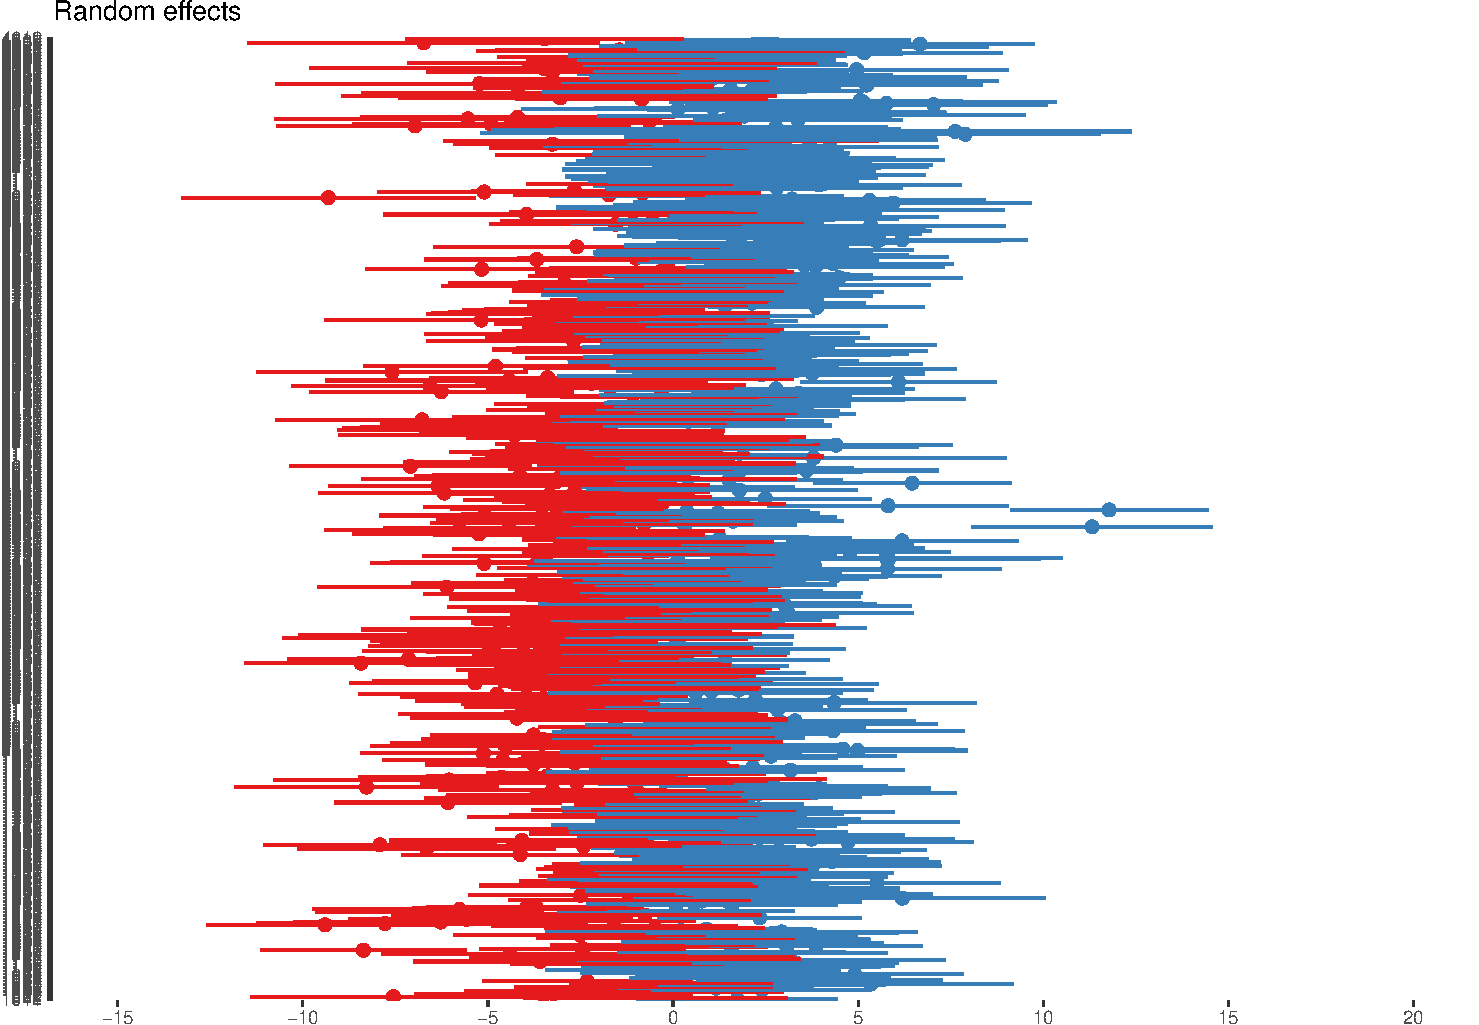
\includegraphics{ancova_01_deck_files/figure-beamer/plotre3-1.pdf}

\end{frame}

\begin{frame}[fragile]{}

Let's plot the estimated school-specific lines from the random intercept
model.

\begin{Shaded}
\begin{Highlighting}[]
\NormalTok{xplot=}\KeywordTok{seq}\NormalTok{(}\OperatorTok{-}\FloatTok{2.9}\NormalTok{,}\FloatTok{2.3}\NormalTok{,}\DataTypeTok{by=}\NormalTok{.}\DecValTok{1}\NormalTok{)}
\NormalTok{yplot=}\KeywordTok{rep}\NormalTok{(}\DecValTok{60}\NormalTok{,}\KeywordTok{length}\NormalTok{(xplot))}
\KeywordTok{plot}\NormalTok{(xplot,yplot,}\DataTypeTok{type=}\StringTok{"n"}\NormalTok{,}\DataTypeTok{ylim=}\KeywordTok{c}\NormalTok{(}\DecValTok{30}\NormalTok{,}\DecValTok{70}\NormalTok{),}\DataTypeTok{xlab=}\StringTok{"Standardized SES"}\NormalTok{,}\DataTypeTok{ylab=}\StringTok{"Math Score"}\NormalTok{)}
\ControlFlowTok{for}\NormalTok{(school }\ControlFlowTok{in} \DecValTok{1}\OperatorTok{:}\KeywordTok{length}\NormalTok{(id.schools))}
\NormalTok{\{}
\NormalTok{  yplot=}\KeywordTok{coef}\NormalTok{(m5)}\OperatorTok{$}\NormalTok{school[school,}\DecValTok{1}\NormalTok{]}\OperatorTok{+}\KeywordTok{coef}\NormalTok{(m5)}\OperatorTok{$}\NormalTok{school[school,}\DecValTok{2}\NormalTok{]}\OperatorTok{*}\NormalTok{xplot}
  \KeywordTok{lines}\NormalTok{(xplot,yplot)}
\NormalTok{\}}
\end{Highlighting}
\end{Shaded}

\end{frame}

\begin{frame}{}

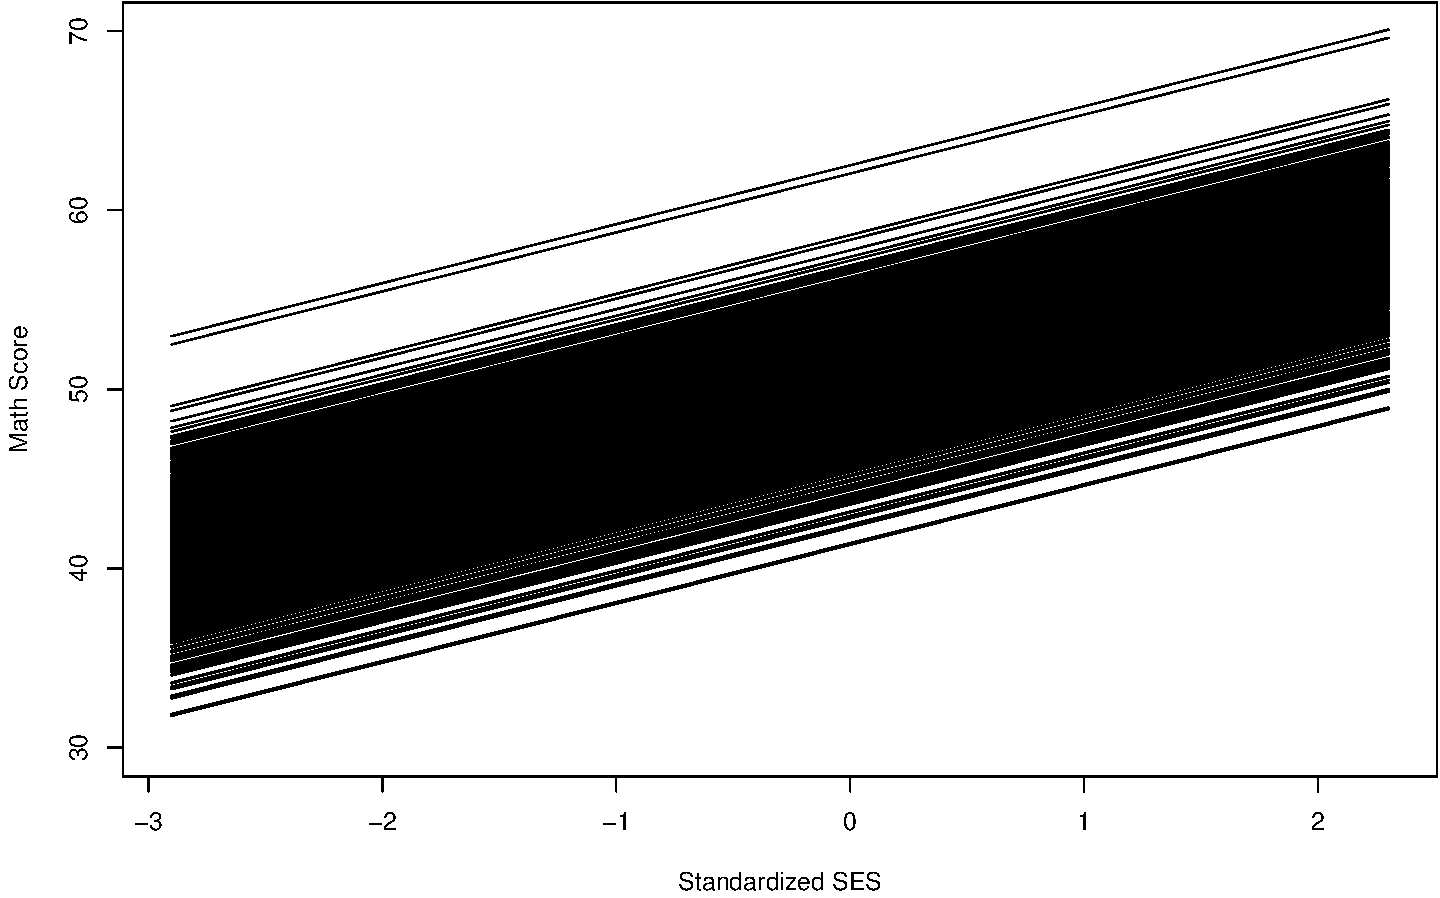
\includegraphics{ancova_01_deck_files/figure-beamer/schoolspecific1b-1.pdf}

\end{frame}

\begin{frame}{}

This model allows separate intercepts for each school but assumes a
common slope. One concern is whether SES has the same relationship with
math scores in all schools. For example, some schools may have less of a
disparity in scores across levels of SES than others.

As an initial step, we can examine at variation in slopes across 100
separate regression models fit separately in each school:
\(y_{ij}=\beta_{0,j}+\beta_{1,j}x_{ij}+\varepsilon_{ij}, ~~ \varepsilon_{ij} \sim N(0,\sigma^2_j)\),
so that in each case \(\widehat{\beta}_j=(X_j'X_j)^{-1}X_j'y_j\), where
here \(X_j\) contains a column of 1's for the intercept and a column
containing the SES of each student.

\end{frame}

\begin{frame}{}

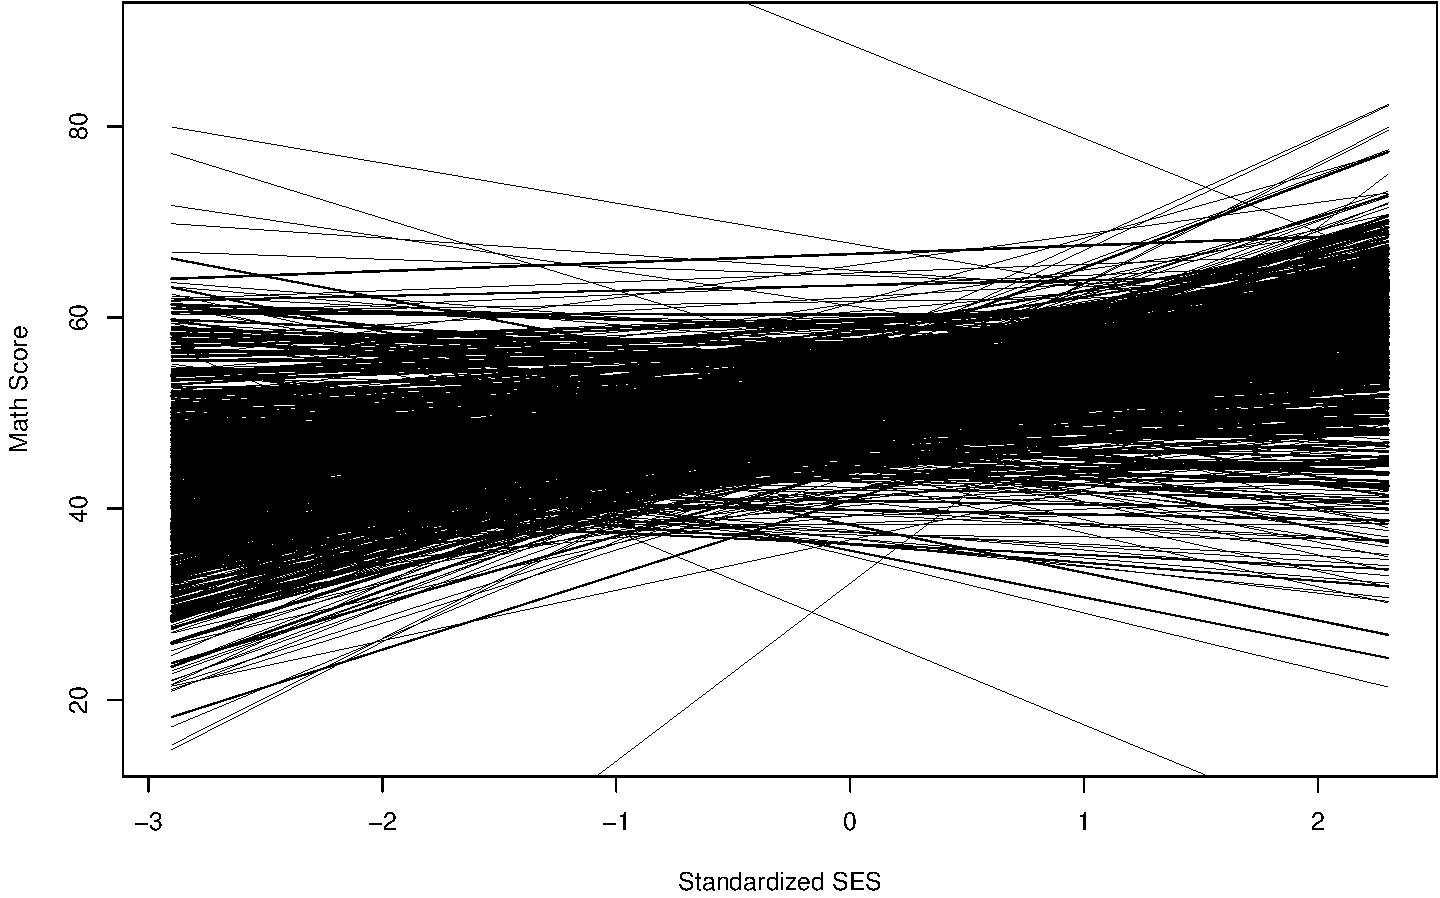
\includegraphics{ancova_01_deck_files/figure-beamer/schoolspecific2b-1.pdf}

This plot looks pretty different!

\end{frame}

\begin{frame}{Histograms of school-specific intercepts and slopes}

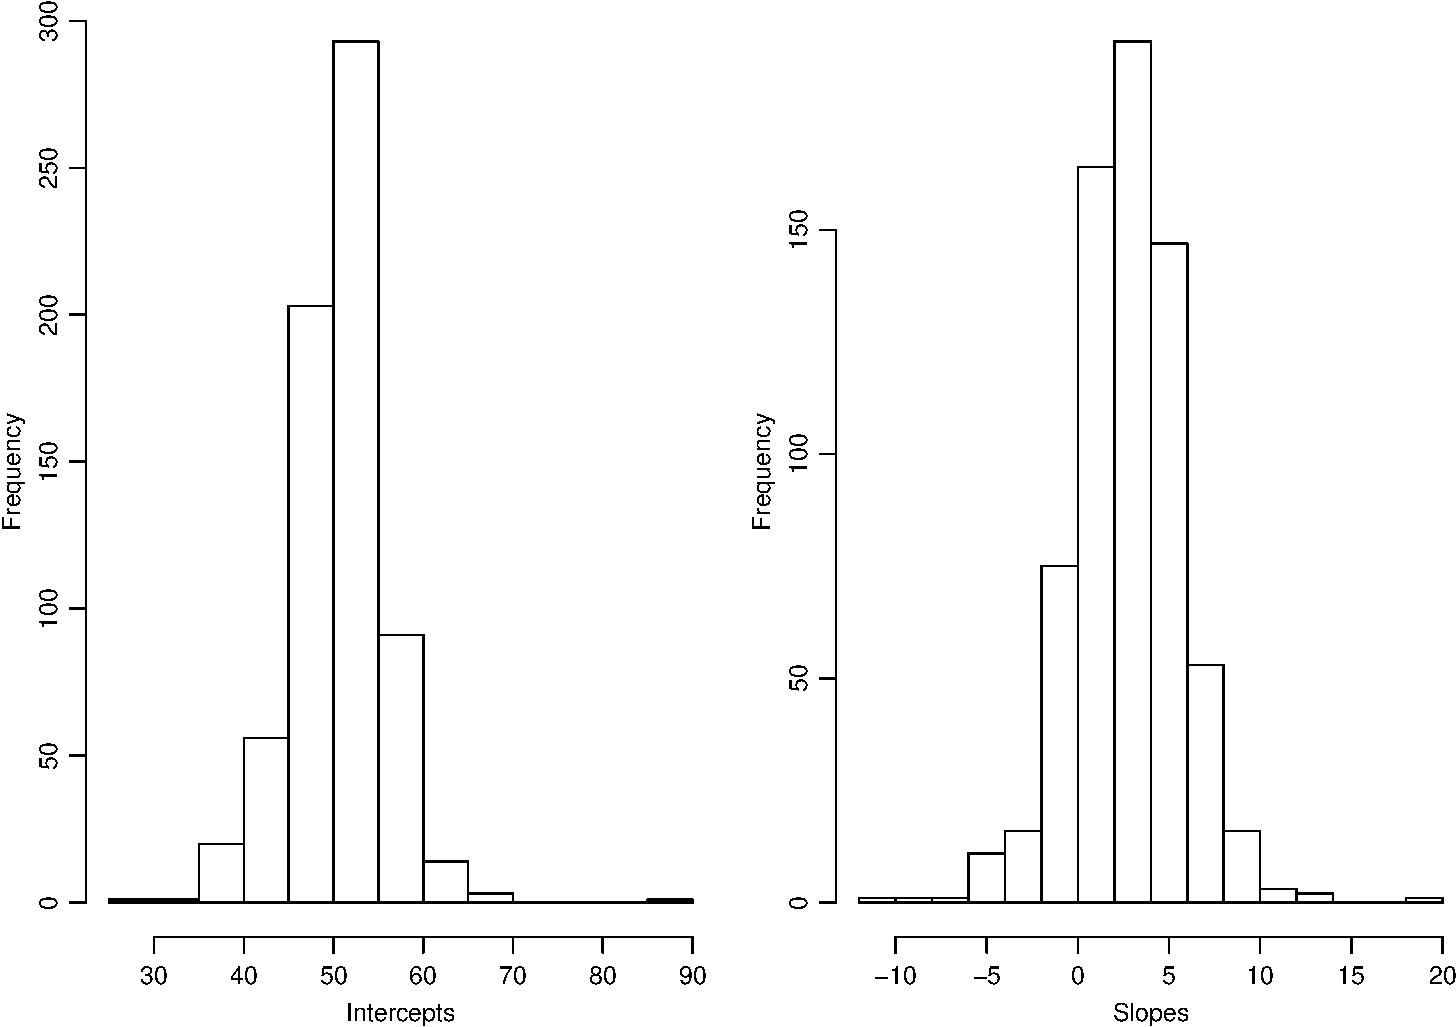
\includegraphics{ancova_01_deck_files/figure-beamer/hist-1.pdf}

\end{frame}

\begin{frame}{}

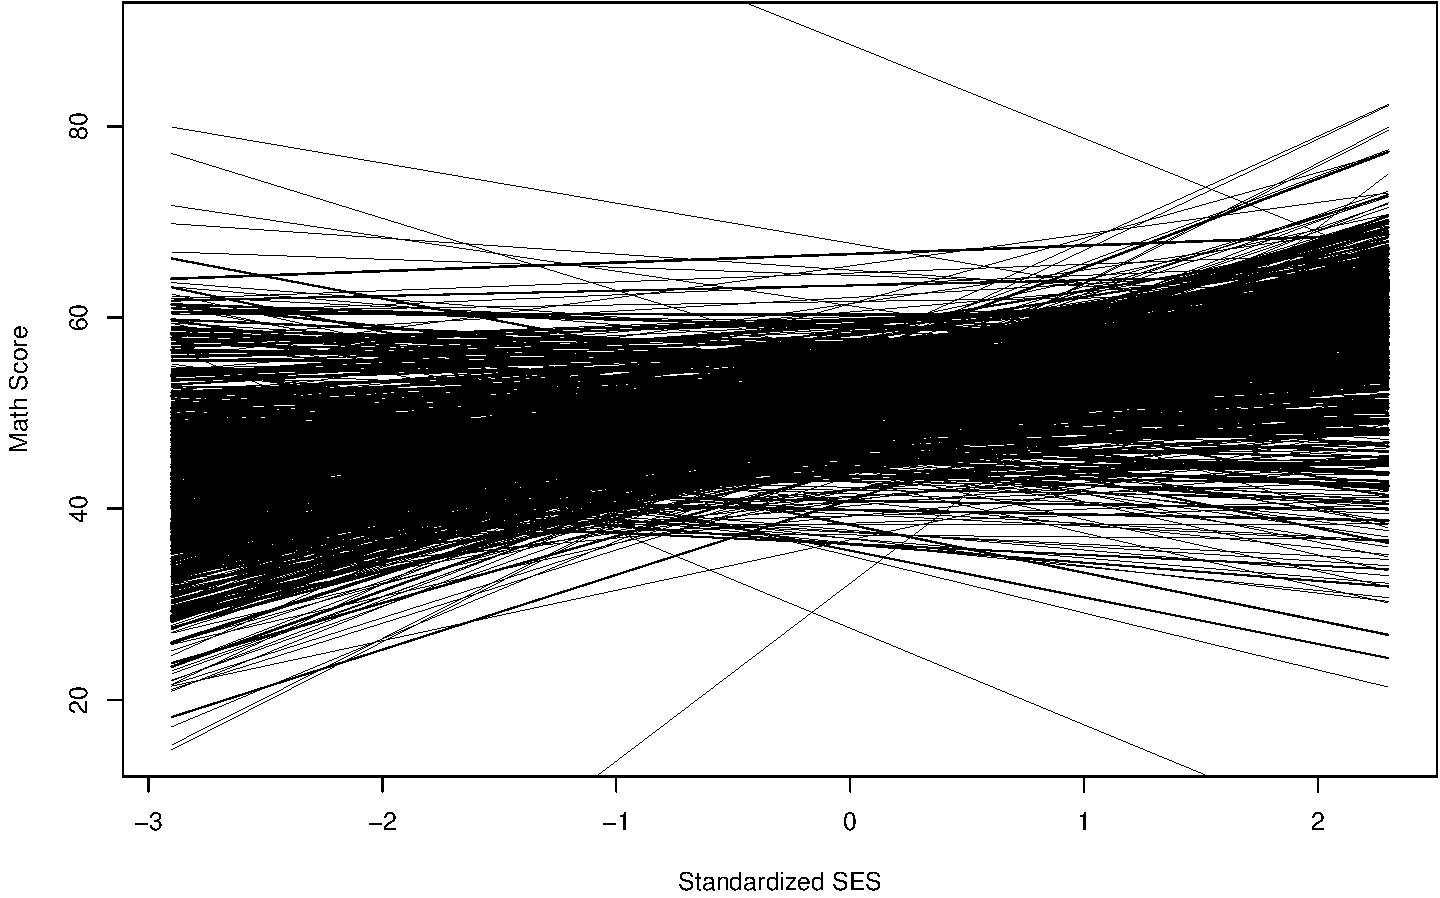
\includegraphics[width=0.5\linewidth]{ancova_01_deck_files/figure-beamer/schoolspecific2c-1}

Line width is proportional to the number of students tested in each
school.

Of the 100 schools, 81 slopes are positive and 19 are negative. The
steepest slopes (positive and negative) tend to occur in the schools
with smaller sample sizes.

How do we get good estimates of the school-specific slopes?

\end{frame}

\begin{frame}{School-specific slopes}

Building on our knowledge of random intercept models, we could consider
the following estimates.

\begin{itemize}
\item
  \(\widehat{\beta}_j=\widehat{\beta}_j^{OLS}=(X_j'X_j)^{-1}X_j'y_j\),
  relying only on the data from school \(j\)
\item
  \(\widehat{\beta}_j=\widehat{\beta}^{POOL}=(X'X)^{-1}X'y\), using all
  the data and pooling across schools
\item
  \(\widehat{\beta}_j=w_j\widehat{\beta}_j^{OLS} + (1-w_j)\widehat{\beta}^{POOL}\),
  doing something in between
\end{itemize}

\end{frame}

\begin{frame}{School-specific slopes}

One alternative to separate linear regression models for each school is
fitting a single model with school-specific slopes and intercepts. These
factors could be fixed or random effects. First, let's consider the
fixed effects approach.

\[y_{ij}=\beta_{0,j}+\beta_{1,j}x_{ij}+\varepsilon_{ij}, ~~~ \varepsilon_{ij} \sim N(0,\sigma^2)\]

If we wish to evaluate whether there is heterogeneity across schools, an
easy approach is to fit the model as a linear regression using indicator
variables as follows.

\end{frame}

\begin{frame}{}

\[y_{ij}=\beta_0+\alpha_jI(\text{school}=j) + \beta_1x_{ij} + \gamma_jx_{ij}I(\text{school}=j) + \varepsilon_{ij},\]
where we assume \(\alpha_J=\gamma_J=0\) (reference cell coding).

In this case, a (J-1) df test can be used to evaluate the hypothesis

\[H_0: \gamma_j=0,~~~ j=1,\ldots,J-1,\]

which corresponds to a constant effect of SES, \(\beta_1\), across
groups.

\end{frame}

\begin{frame}[fragile]{}

\begin{Shaded}
\begin{Highlighting}[]
\NormalTok{m6=}\KeywordTok{lm}\NormalTok{(nels_mathdat}\OperatorTok{$}\NormalTok{mscore}\OperatorTok{~}\KeywordTok{as.factor}\NormalTok{(nels_mathdat}\OperatorTok{$}\NormalTok{school)}\OperatorTok{+}\NormalTok{nels_mathdat}\OperatorTok{$}\NormalTok{sesstd) }\CommentTok{#pooled slope}
\NormalTok{m7=}\KeywordTok{lm}\NormalTok{(nels_mathdat}\OperatorTok{$}\NormalTok{mscore}\OperatorTok{~}\KeywordTok{as.factor}\NormalTok{(nels_mathdat}\OperatorTok{$}\NormalTok{school)}\OperatorTok{+}\NormalTok{nels_mathdat}\OperatorTok{$}\NormalTok{sesstd}\OperatorTok{+}\KeywordTok{as.factor}\NormalTok{(nels_mathdat}\OperatorTok{$}\NormalTok{school)}\OperatorTok{*}\NormalTok{nels_mathdat}\OperatorTok{$}\NormalTok{sesstd) }\CommentTok{#school-specific slopes}
\NormalTok{LR=}\DecValTok{2}\OperatorTok{*}\NormalTok{(}\KeywordTok{logLik}\NormalTok{(m7)}\OperatorTok{-}\KeywordTok{logLik}\NormalTok{(m6))}
\DecValTok{1}\OperatorTok{-}\KeywordTok{pchisq}\NormalTok{(LR,}\DecValTok{201}\OperatorTok{-}\DecValTok{102}\NormalTok{)}
\end{Highlighting}
\end{Shaded}

\begin{verbatim}
## 'log Lik.' 0 (df=1368)
\end{verbatim}

Here we have evidence in favor of school-specific slopes in the fixed
effects model. However, our estimates of school-specific slopes in small
schools may have high variance.

\end{frame}

\begin{frame}{}

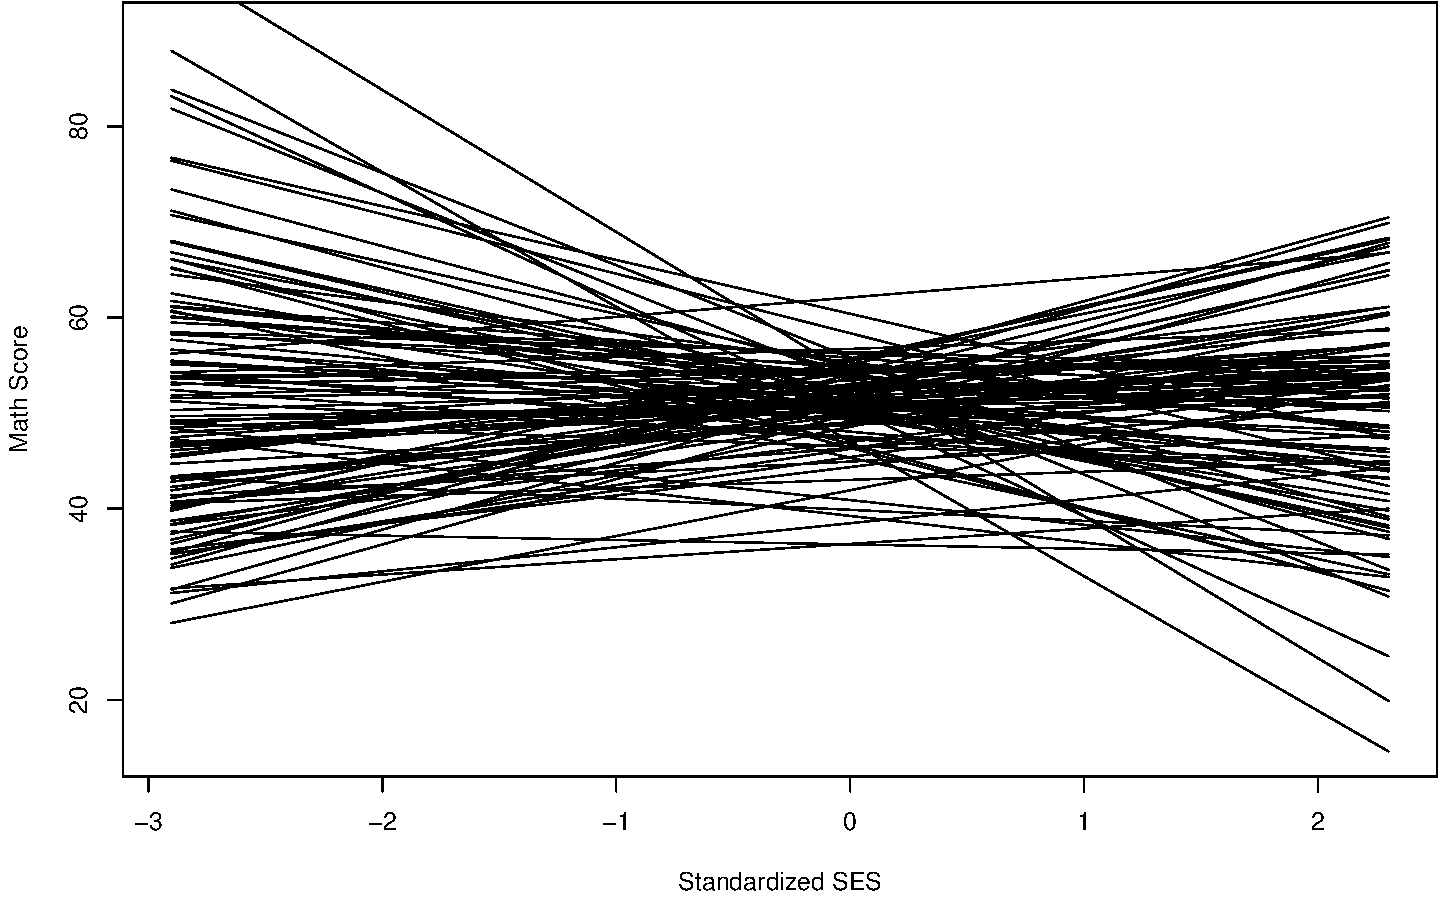
\includegraphics{ancova_01_deck_files/figure-beamer/plotslopes-1.pdf}

The only difference from the models used to obtain the prior lines is
that in this case we estimated a common variance.

\end{frame}

\begin{frame}{}

How should we estimate \(\beta_j\)? Is this pattern becoming familiar?

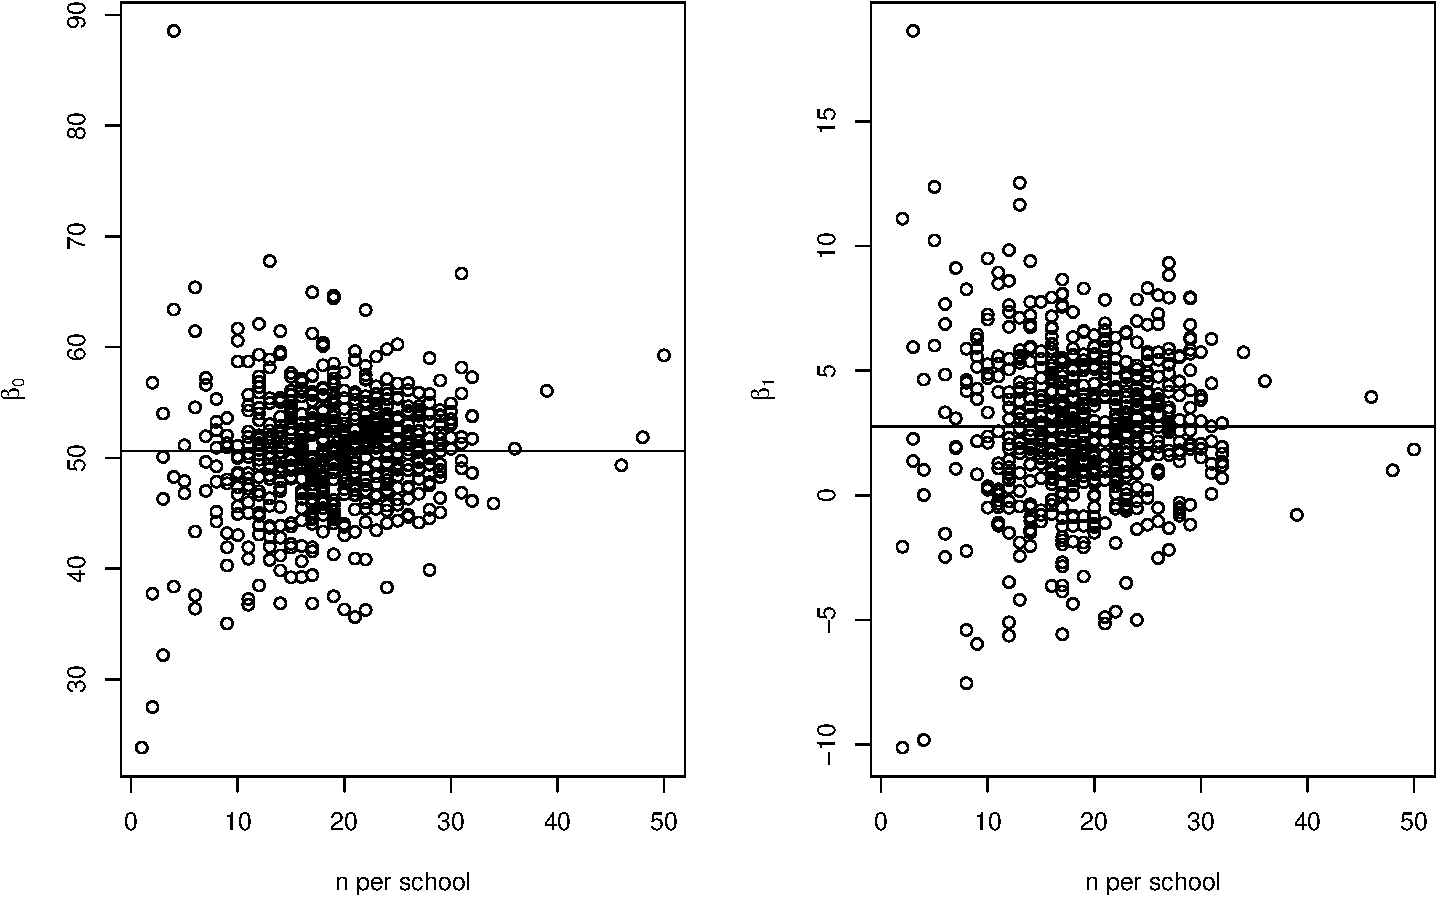
\includegraphics{ancova_01_deck_files/figure-beamer/betasbyn-1.pdf}

\end{frame}

\begin{frame}{Hierarchical Regression Models}

Our hierarchical normal model involves two levels:

\begin{itemize}
\tightlist
\item
  within-group model \(p(y_{1j},\ldots,y_{n_jj} \mid \theta_j)\)
  describing heterogeneity in group j
\item
  among-groups model \(p(\theta_1,\ldots,\theta_J)\)
\end{itemize}

Specifically, we let

\begin{itemize}
\tightlist
\item
  \(\theta_j=(\mu_j, \sigma^2)\)
\item
  \(y_{1j}, \ldots y_{n_jj} \mid \theta \overset{iid}{\sim}N\left(\mu_j, \sigma^2\right)\)
\item
  \(\mu_1,\ldots,\mu_j \overset{iid}{\sim}N\left(\mu, \tau^2\right)\)
\end{itemize}

\end{frame}

\begin{frame}{}

In the regression setting, we have

\begin{itemize}
\tightlist
\item
  \(\theta_j=(\beta_j, \sigma^2)\)
\item
  \(y_{ij}=\beta_j'x_{ij}+\varepsilon_{ij}, ~~ \varepsilon_{ij} \overset{iid}{\sim} N\left(0,\sigma^2\right)\)
\item
  \(\beta_1, \ldots, \beta_J \overset{iid}{\sim} p(\beta_j)\)
\end{itemize}

How should we model \(p(\beta_j)\), the heterogeneity across groups in
the vector of regression coefficients?

\end{frame}

\begin{frame}{}

It is often the case that intercepts and slopes are correlated.

\begin{itemize}
\tightlist
\item
  In a study of income over time, people who start off making more money
  may have larger raises over time.
\item
  In a study of exercise, people who exercise a lot at the start of the
  study may have lower changes over time than those who exercise less
\end{itemize}

A natural choice for the \(\beta_j\) model is the multivariate normal
distribution, which allows for correlation among the group-specific
regression coefficients.

\end{frame}

\begin{frame}{}

We can specify our model in the context of maximum likelihood estimation
as

\begin{itemize}
\tightlist
\item
  \(y_j \mid \beta_j \sim MVN(X_j\beta_j, \sigma^2I)\)
\item
  \(\beta_j \sim MVN(\beta,\Sigma_\beta)\)
\end{itemize}

\(\beta_j \sim MVN(\beta,\Sigma_\beta) \iff \beta_j=\beta+b_j, ~~ b_j \sim MVN(0, \Sigma_\beta)\)

The parameters are

\begin{itemize}
\tightlist
\item
  \(\beta\), an across-group mean vector of regression coefficients
\item
  \(\Sigma_\beta\), a covariance matrix describing the variability of
  the \(\beta_j\) around \(\beta\)
\end{itemize}

\end{frame}

\begin{frame}{}

We can combine terms and write the model as

\[y_j=X_j\beta_j+\varepsilon_j=X_j(\beta+b_j)+\varepsilon_j=X_j\beta+X_jb_j+\varepsilon_j\]

Here

\begin{itemize}
\tightlist
\item
  \(\beta\) is sometimes called a fixed effect (fixed across all groups)
\item
  \(b_j\) is sometimes called a random effect (varies across groups and
  can be considered random if groups were randomly sampled)
\item
  a model with both fixed and random effects is often called a
  mixed-effects model
\end{itemize}

\end{frame}

\begin{frame}[fragile]{\emph{Ad hoc} estimates}

We can get a rough estimate of \(\beta\) by averaging the estimates from
our 100 school-specific regression models.

\begin{Shaded}
\begin{Highlighting}[]
\KeywordTok{apply}\NormalTok{(BETA.OLS,}\DecValTok{2}\NormalTok{,mean)}
\end{Highlighting}
\end{Shaded}

\begin{verbatim}
## (Intercept)          xj 
##    50.61823          NA
\end{verbatim}

This estimator is not perfect -- it equally weights all the schools,
regardless of size. We would prefer to assign a lower weight to schools
with less data.

\end{frame}

\begin{frame}[fragile]{\emph{Ad hoc} estimates}

We can get a \emph{very rough} estimate of \(\Sigma_\beta\):

\begin{Shaded}
\begin{Highlighting}[]
\KeywordTok{cov}\NormalTok{(BETA.OLS,}\DataTypeTok{use=}\StringTok{"complete.obs"}\NormalTok{) }\CommentTok{#dropped n=1 schools}
\end{Highlighting}
\end{Shaded}

\begin{verbatim}
##             (Intercept)        xj
## (Intercept)  26.7958507 0.7529181
## xj            0.7529181 8.9391754
\end{verbatim}

This estimate not only ignores sample size differences, it also ignores
the variability of \(\widehat{\beta}_j\) around \(\beta_j\):
\[\text{Var}[\widehat{\beta}_j\text{'s around }\widehat{\beta}] \approx \text{Var}[\beta_j\text{'s around }\beta]+\text{Var}[\widehat{\beta}_j\text{'s around }\beta_j\text{'s}]:\]

basically, the sample covariance of the \(\widehat{\beta}_j\)'s is
approximately \[\Sigma_\beta +  \text{estimation error}\]

\end{frame}

\begin{frame}{Covariance within Groups}

\(Cov(y_j)=E[(y_j-E(y_j))(y_j-E(y_j))']\)

In our model
\[y_j=X_j\beta_j+\varepsilon_j=X_j(\beta+b_j)+\varepsilon_j=X_j\beta+x_jb_j+\varepsilon_j\],
\[y_j-E[y_j]=y_j-X_j\beta=X_jb_j+\varepsilon_j,~~ $b_j \sim N(0,\Sigma_\beta), ~~\varepsilon_j \sim N(0,\sigma^2I)\]
and because we specify \(b_j \perp \varepsilon_j\),
\[Cov(y_j)=E[(X_jb_j+\varepsilon_j)(X_jb_j+\varepsilon_j)']\]
\[=E[X_jb_jb_j'X_j']+E[\varepsilon_j\varepsilon_j']=X_j\Sigma_\beta X_j'+\sigma^2I.\]

\end{frame}

\begin{frame}{Marginal and conditional distributions of \(y\)}

So conditional on \(b_j\), \[y_j \sim MVN(X_j\beta+X_jb_j, \sigma^2I)\]
and unconditional on \(b_j\) we have
\[p(y_j \mid \beta, \Sigma_\beta, \sigma^2)=MVN(X_j\beta, X_j\Sigma_\beta X_j' + \sigma^2I).\]

\end{frame}

\begin{frame}{Dependence and conditional independence}

Marginal dependence: If we don't know \(\beta_j\) (or \(b_j\)), then
knowing the response \(y_{ij}\) gives me some information about
\(\beta_j\), which gives us some information about \(y_{i'j}\), so the
observations within a group are dependent.

Conditional independence: If I do know \(\beta_j\), then knowing
\(y_{ij}\) does not give me any extra information about \(y_{i'j}\), and
they are independent. My information about \(y_{ij} \perp y_{i'j}\) if I
know \(\beta_j\).

\end{frame}

\begin{frame}[fragile]{Fitting the model}

\begin{Shaded}
\begin{Highlighting}[]
\CommentTok{#recall g.nels is the sequential ID variable}
\NormalTok{m8=}\KeywordTok{lmer}\NormalTok{(nels_mathdat}\OperatorTok{$}\NormalTok{mscore}\OperatorTok{~}\NormalTok{nels_mathdat}\OperatorTok{$}\NormalTok{sesstd}\OperatorTok{+}\NormalTok{(nels_mathdat}\OperatorTok{$}\NormalTok{sesstd}\OperatorTok{|}\NormalTok{g.nels),}\DataTypeTok{REML=}\OtherTok{FALSE}\NormalTok{)}
\KeywordTok{summary}\NormalTok{(m8)}
\end{Highlighting}
\end{Shaded}

\begin{verbatim}
## Linear mixed model fit by maximum likelihood  ['lmerMod']
## Formula: 
## nels_mathdat$mscore ~ nels_mathdat$sesstd + (nels_mathdat$sesstd |  
##     g.nels)
## 
##      AIC      BIC   logLik deviance df.resid 
##  92553.1  92597.9 -46270.5  92541.1    12968 
## 
## Scaled residuals: 
##     Min      1Q  Median      3Q     Max 
## -3.8910 -0.6382  0.0179  0.6669  4.4613 
## 
## Random effects:
##  Groups   Name                Variance Std.Dev. Corr
##  g.nels   (Intercept)         12.2231  3.4961       
##           nels_mathdat$sesstd  0.8562  0.9253   0.11
##  Residual                     67.3451  8.2064       
## Number of obs: 12974, groups:  g.nels, 684
## 
## Fixed effects:
##                     Estimate Std. Error t value
## (Intercept)         50.67670    0.15511   326.7
## nels_mathdat$sesstd  3.27708    0.09256    35.4
## 
## Correlation of Fixed Effects:
##             (Intr)
## nls_mthdt$s 0.007
\end{verbatim}

\end{frame}

\begin{frame}[fragile]{Do we need the random slope in addition to the
random intercept?}

Let's test whether the slope should be random or fixed -- this time the
reference distribution is a 50-50 mixture of \(\chi^2_1\) and
\(\chi^2_2\) distributions. This is a test of the hypothesis that the
variance of the random slope is zero.

\begin{Shaded}
\begin{Highlighting}[]
\NormalTok{LR=}\KeywordTok{logLik}\NormalTok{(}\KeywordTok{lmer}\NormalTok{(mscore}\OperatorTok{~}\NormalTok{(}\DecValTok{1}\OperatorTok{|}\NormalTok{school),}\DataTypeTok{data=}\NormalTok{nels_mathdat,}\DataTypeTok{REML=}\OtherTok{FALSE}\NormalTok{))}
 \OperatorTok{-}\KeywordTok{logLik}\NormalTok{(}\KeywordTok{lmer}\NormalTok{(mscore}\OperatorTok{~}\NormalTok{sesstd}\OperatorTok{+}\NormalTok{(sesstd}\OperatorTok{|}\NormalTok{school),}
              \DataTypeTok{data=}\NormalTok{nels_mathdat,}\DataTypeTok{REML=}\OtherTok{FALSE}\NormalTok{))}
\end{Highlighting}
\end{Shaded}

\begin{verbatim}
## 'log Lik.' 46270.53 (df=6)
\end{verbatim}

\begin{Shaded}
\begin{Highlighting}[]
\FloatTok{0.5}\OperatorTok{*}\NormalTok{(}\DecValTok{1}\OperatorTok{-}\KeywordTok{pchisq}\NormalTok{(LR[}\DecValTok{1}\NormalTok{],}\DecValTok{2}\NormalTok{)}\OperatorTok{+}\DecValTok{1}\OperatorTok{-}\KeywordTok{pchisq}\NormalTok{(LR[}\DecValTok{1}\NormalTok{],}\DecValTok{1}\NormalTok{))}
\end{Highlighting}
\end{Shaded}

\begin{verbatim}
## [1] 1
\end{verbatim}

Yes, looks like the random slope explains additional variance.

\end{frame}

\begin{frame}{Comparing estimates}

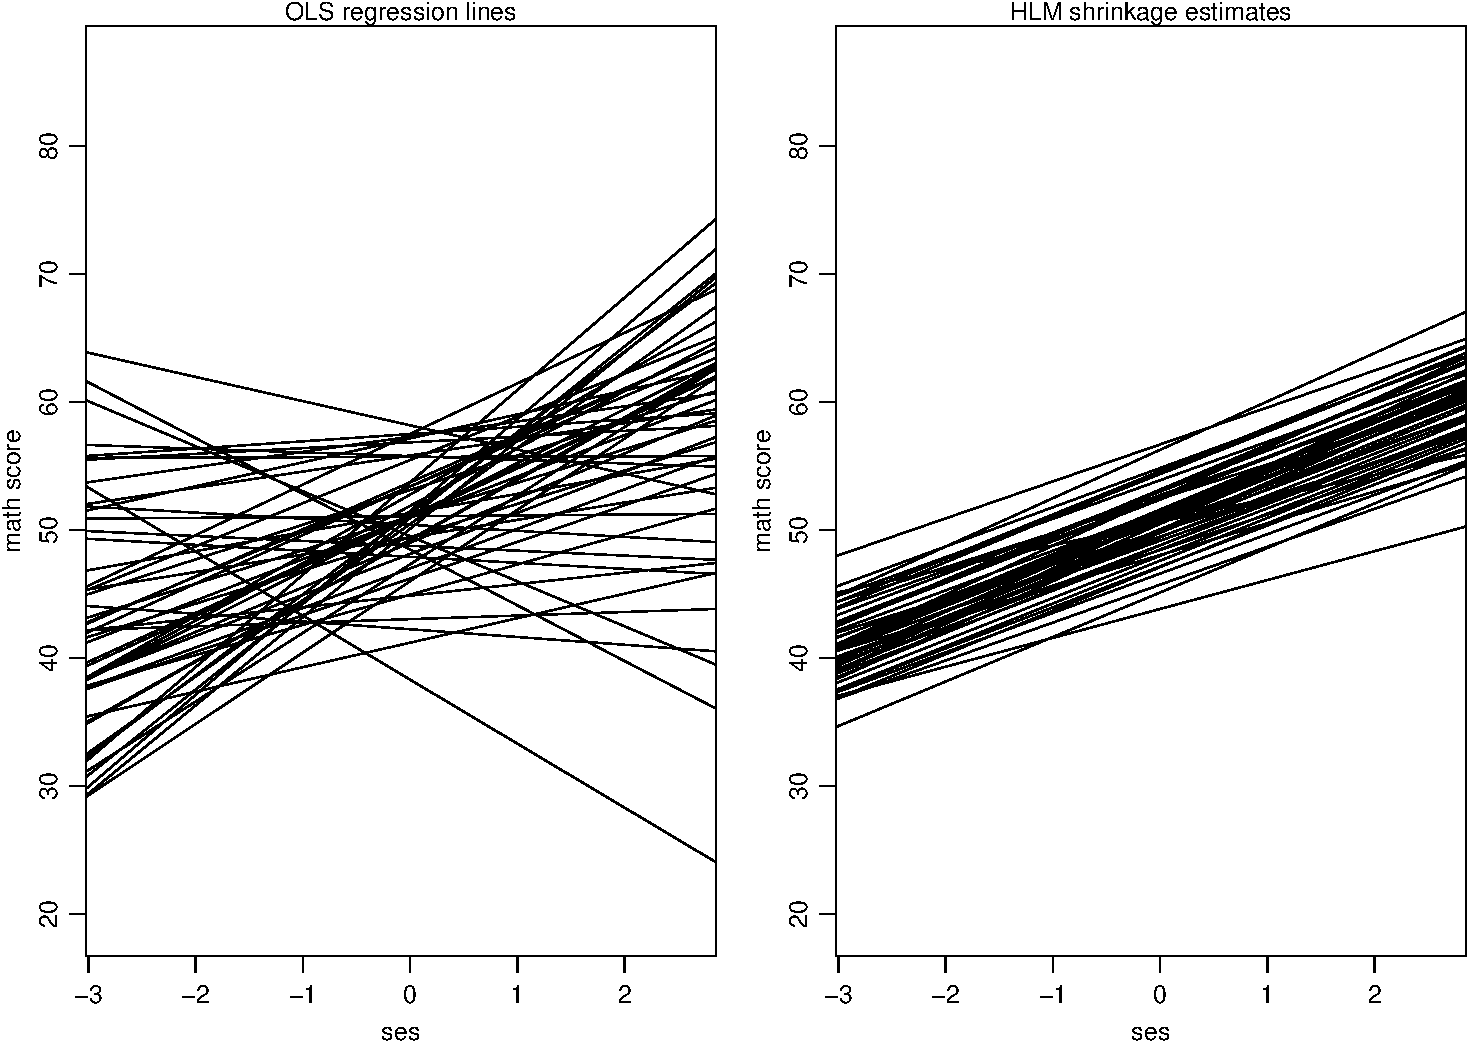
\includegraphics{ancova_01_deck_files/figure-beamer/compest-1.pdf}

\end{frame}

\begin{frame}{Shrinkage Estimates}

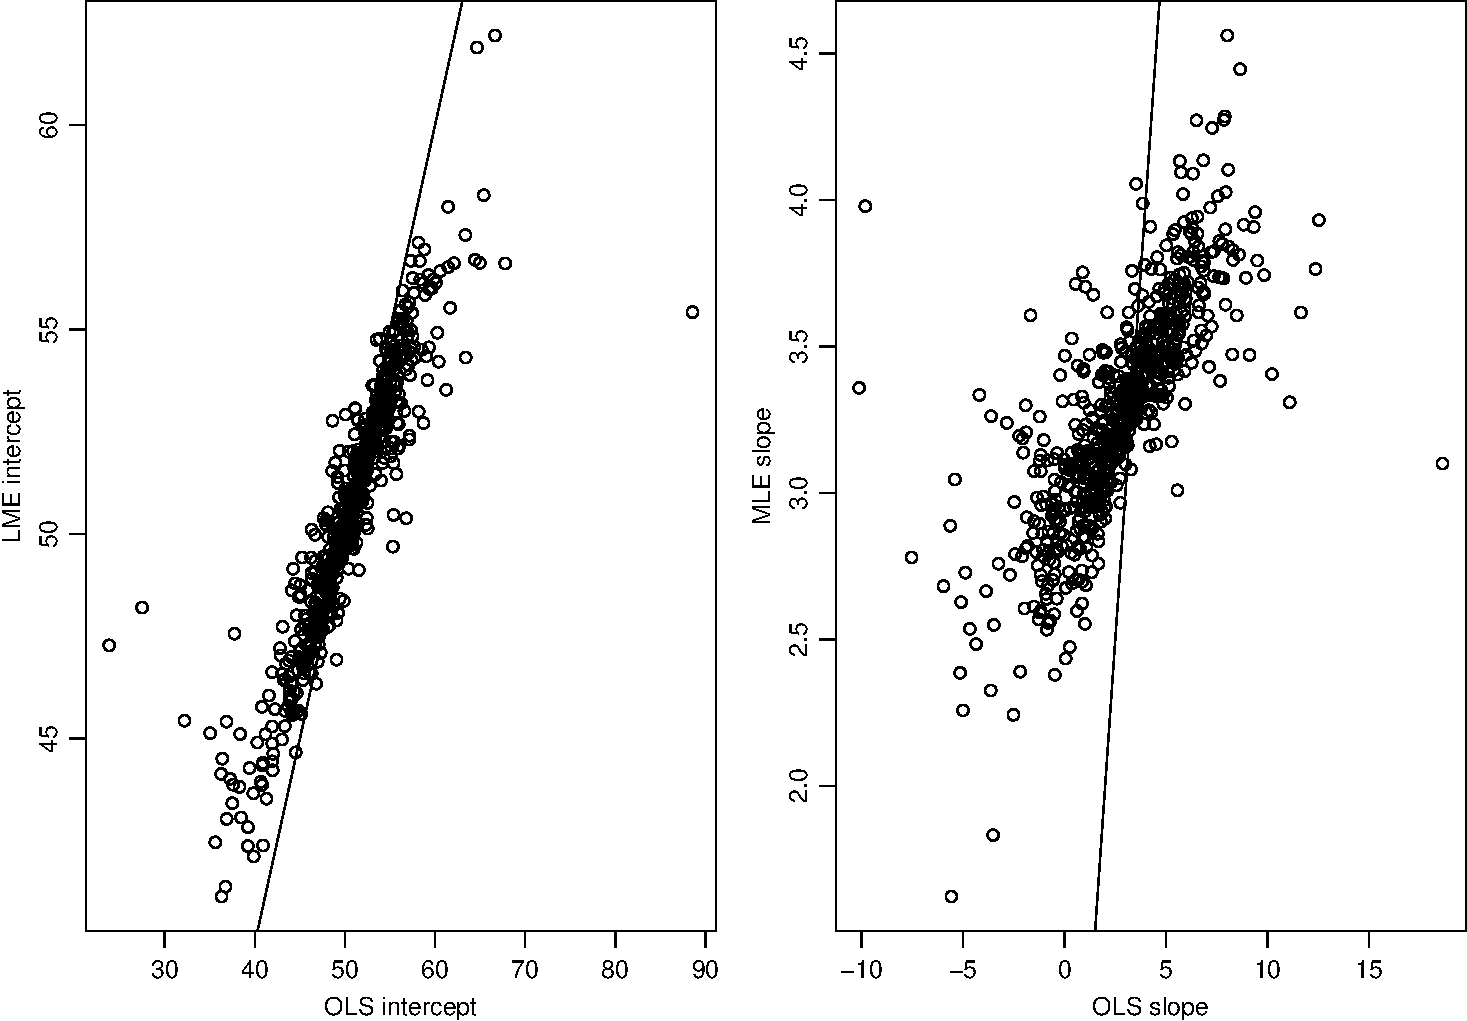
\includegraphics{ancova_01_deck_files/figure-beamer/shrinkydinky-1.pdf}

\end{frame}

\begin{frame}{Shrinkage Estimates}

Intuitively,
\(\widetilde{\beta}_j=w_j\widehat{\beta}_j+(1-w_j)\widehat{\beta}\),
where \(w_j\) is a function of \(\Sigma_\beta\) and
\(\sigma^2(X_j'X_j)^{-1}\):

\begin{itemize}
\tightlist
\item
  \(w_j\) is big if \(\sigma^2(X_j'X_j)^{-1}\) small relative to
  \(\Sigma_\beta\)
\item
  \(w_j\) is small if \(\sigma^2(X_j'X_j)^{-1}\) large relative to
  \(\Sigma_\beta\)
\end{itemize}

This is approximately what happens: the averaging has to be done using
matrices as
\[\widetilde{\beta}_j=\left(X_j'X_j/\sigma^2 + \Sigma_\beta^{-1}\right)^{-1}\left(X_jy_j/\sigma^2+\Sigma_\beta^{-1}\beta \right)\]

\end{frame}

\begin{frame}{What kind of schools have big intercepts and big slopes?}

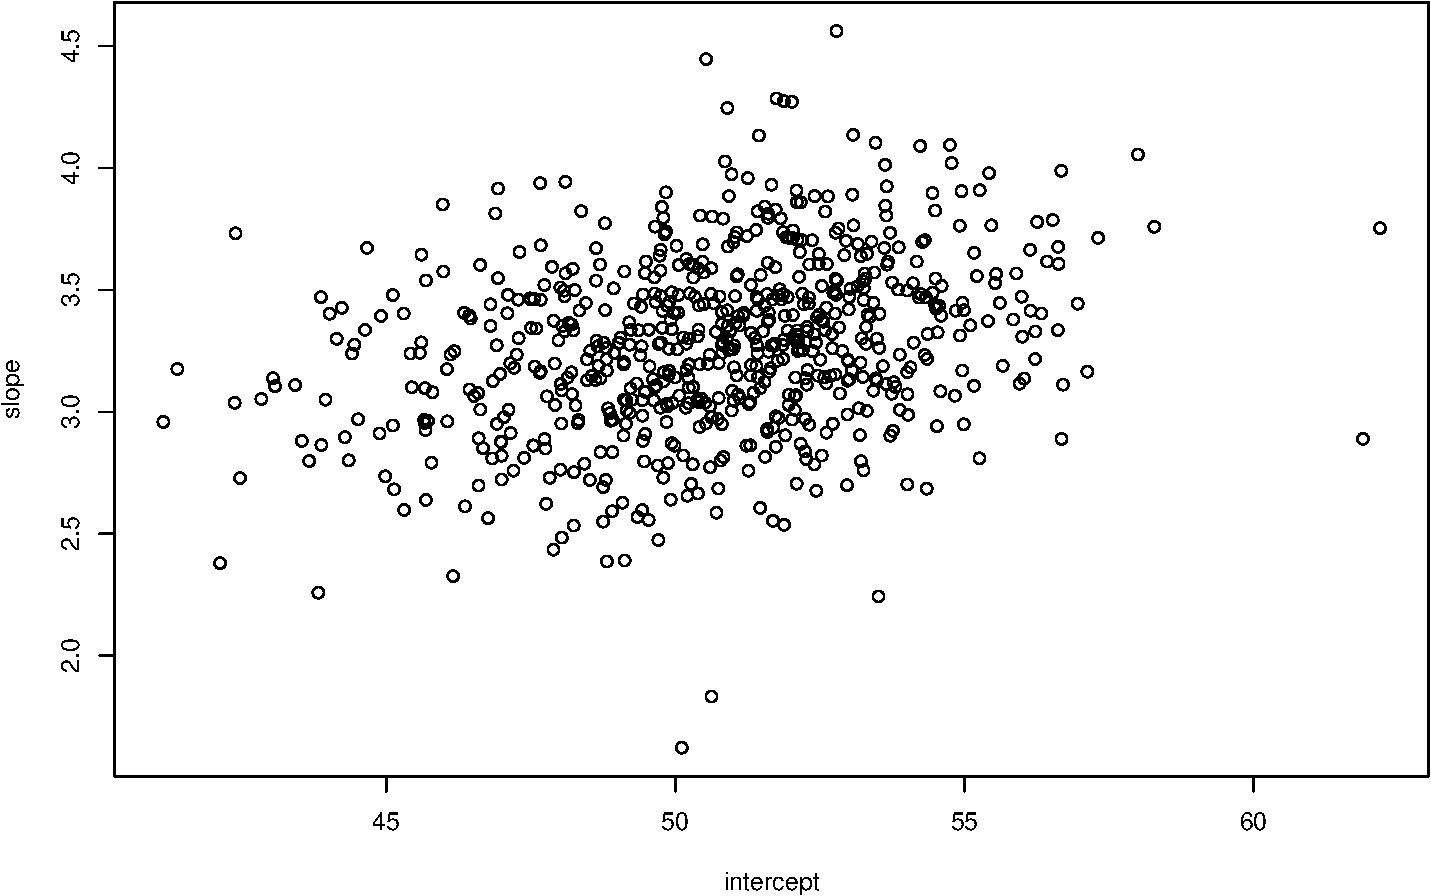
\includegraphics{ancova_01_deck_files/figure-beamer/plotintslope-1.pdf}

We will examine whether a school-level indicator, the percentage of
children eligible for free lunch, will explain additional variability in
school-level intercepts and slopes.

\end{frame}

\begin{frame}{Free Lunch Variable}

The US government has programs to provide free or reduced-price lunches
to students based on their family economic status. The percentage of
children in a school who are eligible to receive free or reduced-price
lunches is an indicator of the school-level socioeconomic status. In our
data, the variable is defined as follows.

\begin{itemize}
\tightlist
\item
  flp=1 if 0-5\% of children are eligible to receive free or
  reduced-price lunch
\item
  flp=2 if 5-30\% of children are eligible for benefits
\item
  flp=3 if \$\textgreater{}\$30\% of children are eligible for benefits
\end{itemize}

\end{frame}

\begin{frame}[fragile]{}

\begin{Shaded}
\begin{Highlighting}[]
\NormalTok{flp.school<-}\KeywordTok{tapply}\NormalTok{( nels_mathdat}\OperatorTok{$}\NormalTok{flp , g.nels, mean) }
\KeywordTok{table}\NormalTok{(flp.school) }

\NormalTok{### RE and FLP association}
\KeywordTok{mpar}\NormalTok{()}
\KeywordTok{par}\NormalTok{(}\DataTypeTok{mfrow=}\KeywordTok{c}\NormalTok{(}\DecValTok{1}\NormalTok{,}\DecValTok{2}\NormalTok{))}
\KeywordTok{boxplot}\NormalTok{(BETA.LME[,}\DecValTok{1}\NormalTok{]}\OperatorTok{~}\NormalTok{flp.school,}\DataTypeTok{col=}\StringTok{"lightblue"}\NormalTok{, }\DataTypeTok{main=}\StringTok{"Intercepts by Lunch"}\NormalTok{) }
\KeywordTok{boxplot}\NormalTok{(BETA.LME[,}\DecValTok{2}\NormalTok{]}\OperatorTok{~}\NormalTok{flp.school,}\DataTypeTok{col=}\StringTok{"lightblue"}\NormalTok{, }\DataTypeTok{main=}\StringTok{"Slopes by Lunch"}\NormalTok{)}
\end{Highlighting}
\end{Shaded}

\end{frame}

\begin{frame}[fragile]{}

\begin{verbatim}
## flp.school
##   1   2   3 
## 226 257 201
\end{verbatim}

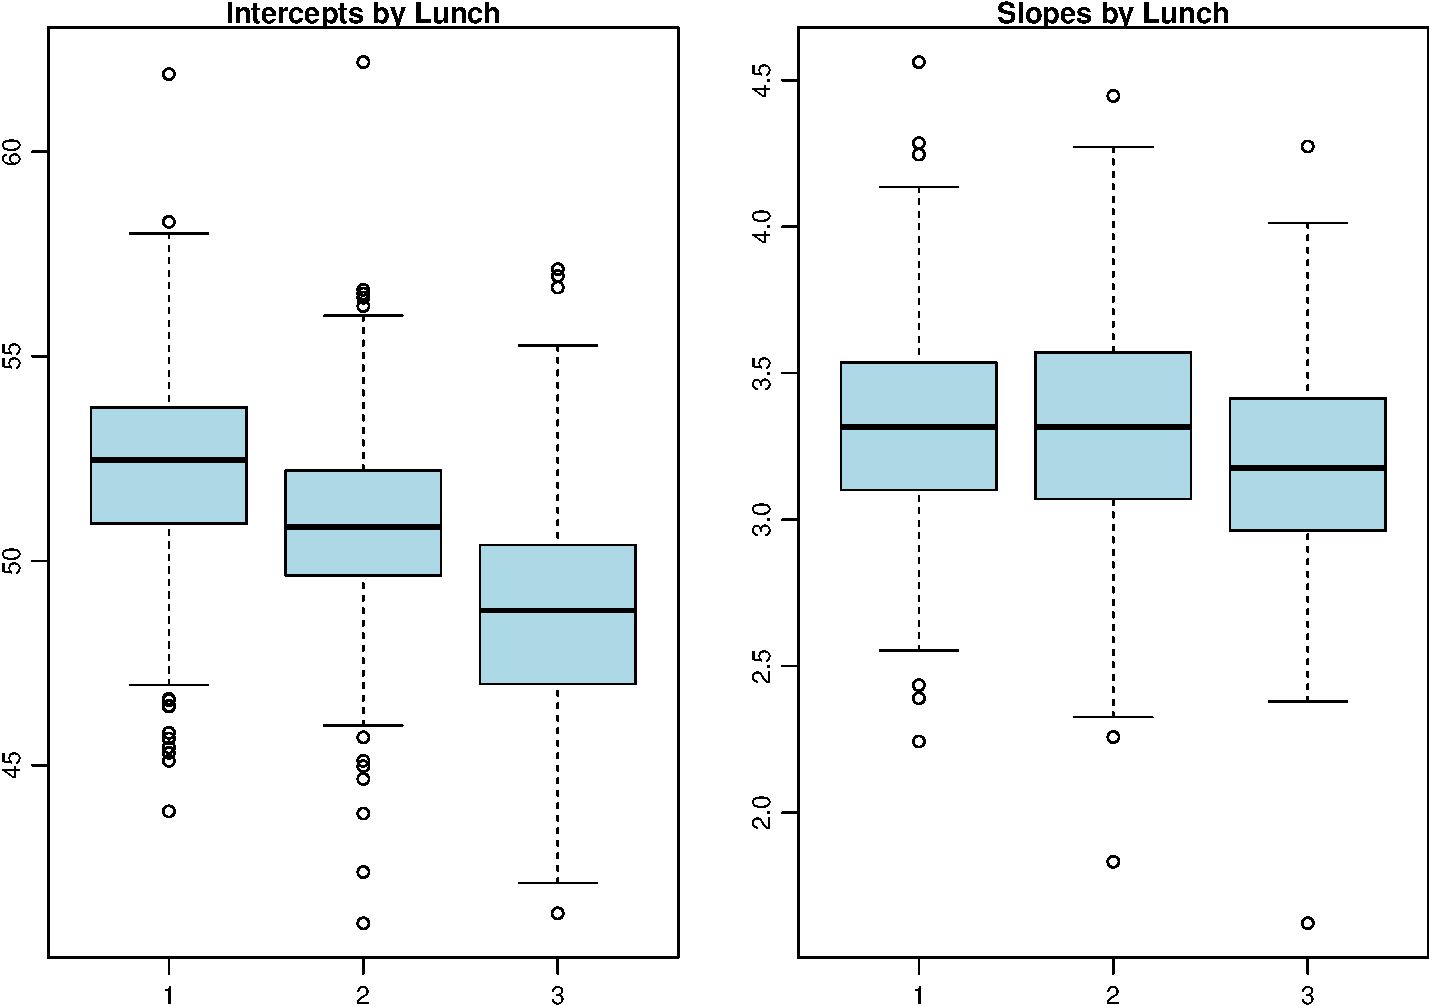
\includegraphics{ancova_01_deck_files/figure-beamer/ses2-1.pdf}

\end{frame}

\begin{frame}{}

Based on the box plots, it seems that the \(\beta_{0,j}\) and maybe the
\(\beta_{1,j}\) are associated with school-level SES, measured by the
percentage of kids eligible for free and reduced-price lunch.

We may be interested in the following:

\begin{itemize}
\tightlist
\item
  Testing: is there evidence of a relationship?
\item
  Estimation: what kind of relationship is there?
\end{itemize}

Let's expand our model so that we can investigate.

\end{frame}

\begin{frame}{Model extension}

Our current model can be written
\[y_{ij}=\beta_{0,j}+\beta_{1,j}\text{ses}_{ij}+\varepsilon_{ij}\] where
\[\beta_{0,j}=\beta_0+b_{0,j} ~~~ \text{and } ~~ \beta_{1,j}=\beta_1+b_{1,j}\]

To investigate whether the school-level SES variable explains additional
variance, we treat it as an ordinal variable (could also treat as
categorical) and expand the models for \(\beta_{h,j}\) so that
\[\beta_{0,j}=\beta_0+\alpha_0\text{flp}_j+b_{0,j} ~~~ \text{and } ~~ \beta_{1,j}=\beta_1+\alpha_1\text{flp}_j+b_{1,j}.\]

Putting things all together, we get

\[y_{ij}=\beta_0+\alpha_0\text{flp}_j+\beta_1\text{ses}_{ij}+\alpha_1\text{flp}_j\text{ses}_{ij}+b_{0,j}+b_{1,j}\text{ses}_{ij}+\varepsilon_{ij}\]

\end{frame}

\begin{frame}{}

Note it does not matter if we use \(\alpha\) or \(\beta\) notationally,
so it may be simpler to write

\[y_{ij}=\beta_0+\beta_1\text{flp}_j+\beta_2\text{ses}_{ij}+\beta_3\text{flp}_j\text{ses}_{ij}+b_{0,j}+b_{1,j}\text{ses}_{ij}+\varepsilon_{ij}\]

or more succinctly,

\[y_j=X_j\beta+Z_jb_j+\varepsilon_j,\] where \(X_j\) is a matrix
containing a column of 1's, a column for flp, and a column for SES, and
\(Z_j\) contains colums for the random intercept and random SES effect.
We'll return to this latter notation in the general context of the
linear mixed effects model.

\end{frame}

\begin{frame}[fragile]{Fitting the model}

\begin{Shaded}
\begin{Highlighting}[]
\KeywordTok{library}\NormalTok{(lme4)}
\NormalTok{m9=}\KeywordTok{lmer}\NormalTok{(nels_mathdat}\OperatorTok{$}\NormalTok{mscore}\OperatorTok{~}\NormalTok{nels_mathdat}\OperatorTok{$}\NormalTok{sesstd}\OperatorTok{+}\NormalTok{nels_mathdat}\OperatorTok{$}\NormalTok{flp}\OperatorTok{+}
\StringTok{          }\NormalTok{nels_mathdat}\OperatorTok{$}\NormalTok{sesstd}\OperatorTok{*}\NormalTok{nels_mathdat}\OperatorTok{$}\NormalTok{flp}\OperatorTok{+}
\StringTok{          }\NormalTok{(nels_mathdat}\OperatorTok{$}\NormalTok{sesstd}\OperatorTok{|}\NormalTok{g.nels),}\DataTypeTok{REML=}\OtherTok{FALSE}\NormalTok{)}
\KeywordTok{summary}\NormalTok{(m9)}
\end{Highlighting}
\end{Shaded}

\end{frame}

\begin{frame}[fragile]{}

\begin{verbatim}
## Linear mixed model fit by maximum likelihood  ['lmerMod']
## Formula: nels_mathdat$mscore ~ nels_mathdat$sesstd + nels_mathdat$flp +  
##     nels_mathdat$sesstd * nels_mathdat$flp + (nels_mathdat$sesstd |  
##     g.nels)
## 
##      AIC      BIC   logLik deviance df.resid 
##  92396.3  92456.0 -46190.1  92380.3    12966 
## 
## Scaled residuals: 
##     Min      1Q  Median      3Q     Max 
## -3.9773 -0.6417  0.0201  0.6659  4.5202 
## 
## Random effects:
##  Groups   Name                Variance Std.Dev. Corr
##  g.nels   (Intercept)          9.0123  3.0020       
##           nels_mathdat$sesstd  0.8881  0.9424   0.06
##  Residual                     67.2595  8.2012       
## Number of obs: 12974, groups:  g.nels, 684
## 
## Fixed effects:
##                                      Estimate Std. Error t value
## (Intercept)                           55.3975     0.3860 143.525
## nels_mathdat$sesstd                    3.3759     0.2501  13.500
## nels_mathdat$flp                      -2.4062     0.1819 -13.230
## nels_mathdat$sesstd:nels_mathdat$flp  -0.1451     0.1193  -1.216
## 
## Correlation of Fixed Effects:
##             (Intr) nls_mthdt$s nls_mthdt$f
## nls_mthdt$s -0.158                        
## nls_mthdt$f -0.930  0.088                 
## nls_mth$:_$  0.086 -0.926      -0.007
\end{verbatim}

\end{frame}

\begin{frame}{Getting More Serious About NELS}

Up to now, we've just used the NELS data to illustrate different aspects
of model fitting for the multilevel model. Now let's step back and think
about these data more holistically, as if we're seeing them for the
first time.

\end{frame}

\begin{frame}{NELS Variables}

We will consider the following variables of interest in NELS.

\begin{itemize}
\tightlist
\item
  Math score (individual-level outcome)
\item
  SES (individual-level socio-economic status)
\item
  FLP (school level \% of kids eligible for free or reduced-price lunch)

  \begin{itemize}
  \tightlist
  \item
    1: 0-5\% eligible
  \item
    2: 5-30\% eligible
  \item
    3: \$\textgreater{}\$30\% eligible
  \end{itemize}
\item
  Enrollment (school level \# of kids in 10th grade, rounded and
  measured in hundreds, so 0=\$\textless{}\$100, 1=around 100, \ldots{},
  5=around 500)
\item
  Public (school level, takes value 1 if public school and 0 if private
  school)
\item
  Urbanicity (school level factor with levels rural, suburban, and urban
  )
\end{itemize}

\end{frame}

\begin{frame}{Model Selection}

As we think about models, we'll keep in mind a couple of methods for
comparison.

\begin{itemize}
\tightlist
\item
  Likelihood ratio test for nested models

  \begin{itemize}
  \tightlist
  \item
    For tests involving fixed effects only, we can use a \(\chi^2_d\)
    for testing whether \(d\) fixed effects all equal 0
  \item
    For tests involving random effects only, we can use a 50-50 mixture
    of \(\chi^2_{p-1}\) and \(\chi^2_p\)
  \item
    Non-nested models or testing both fixed and random effects, not so
    simple
  \end{itemize}
\item
  BIC

  \begin{itemize}
  \tightlist
  \item
    smaller-is-better coding
  \item
    already adjusted for model complexity
  \item
    approximation to posterior model probability
  \item
    model selection consistent
  \item
    nested models not required
  \end{itemize}
\end{itemize}

\end{frame}

\begin{frame}{Descriptive Statistics}

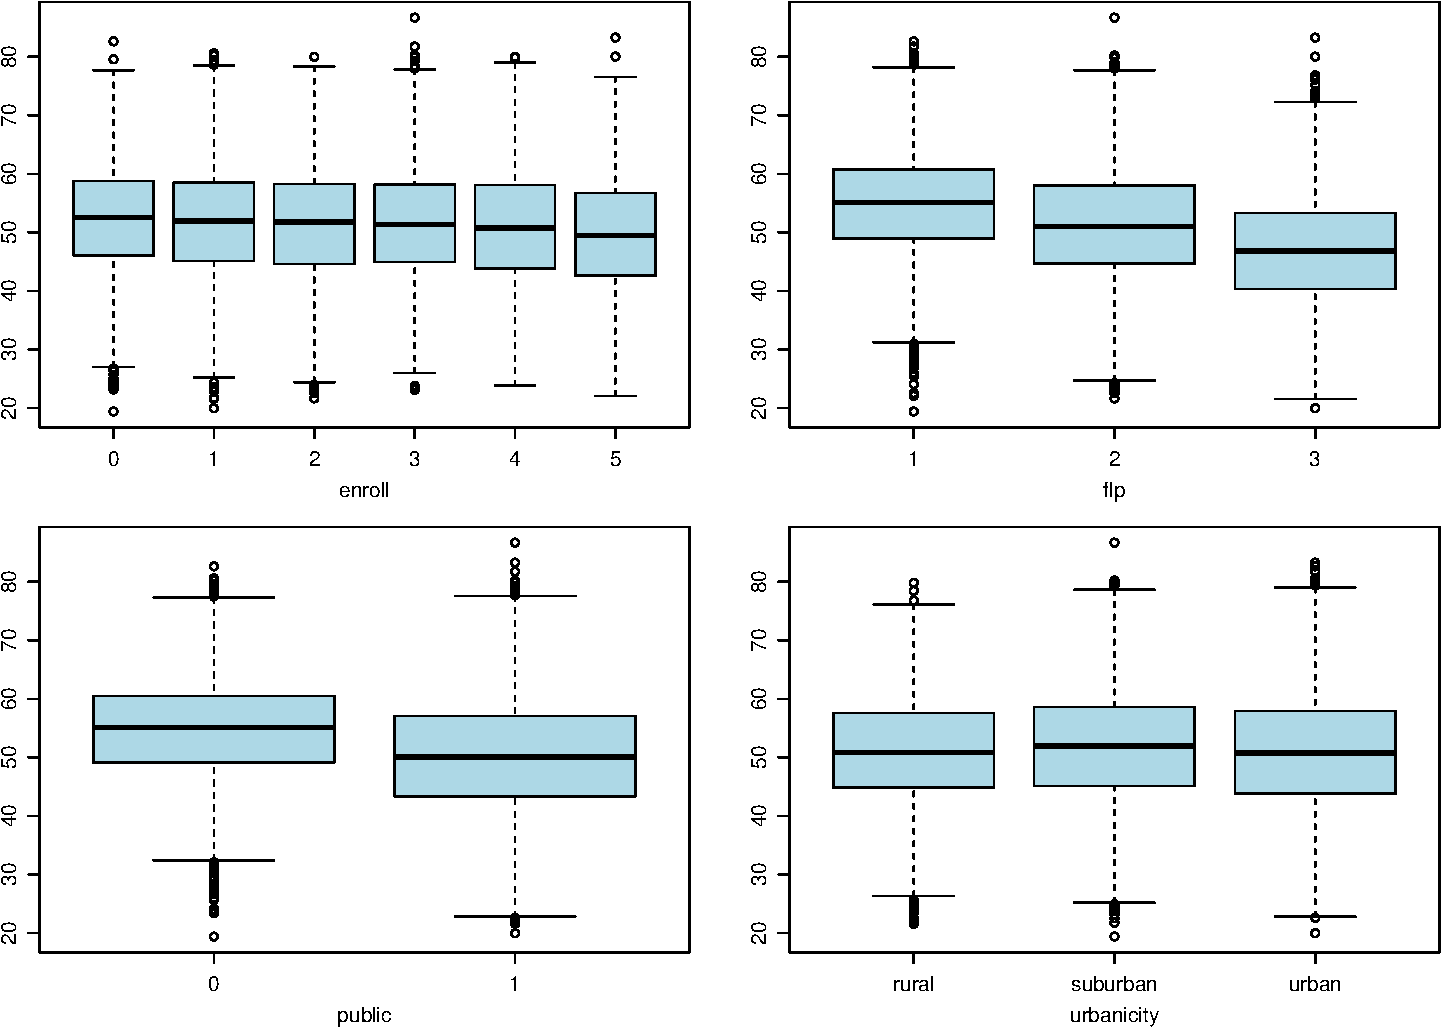
\includegraphics{ancova_01_deck_files/figure-beamer/boxplots-1.pdf}

\end{frame}

\begin{frame}{What's wrong with ANOVA?}

Suppose I don't really care about school effects one way or the other.
Why not just use ANOVA (or other fixed effects model) here?

Under a fixed effects model,
\[\text{Cov}(y_j)=\begin{pmatrix} \sigma^2 & 0 & \ldots & 0 \\ 0 & \sigma^2 & \ldots & 0 \\ \vdots & & \vdots \\ 0 & 0 & \ldots & \sigma^2 \end{pmatrix}\]

\end{frame}

\begin{frame}{}

Under a random intercept model,
\[\text{Cov}(y_j)=\begin{pmatrix} \sigma^2 +\tau^2 & \tau^2 & \ldots & \tau^2 \\ \tau^2 & \sigma^2 + \tau^2 & \ldots & \tau^2 \\ \vdots & & & \vdots \\ \tau^2 & \tau^2 & \ldots & \sigma^2 + \tau^2 \end{pmatrix},\]

and

\(Corr(y_{ij},y_{i'j})=\frac{\tau^2}{\tau^2+\sigma^2}\)

We generally don't believe independence within the same school
environment holds.

\end{frame}

\begin{frame}[fragile]{}

Why not treat school as a fixed effect? That should handle the school
heterogeneity.

\begin{Shaded}
\begin{Highlighting}[]
\NormalTok{m10=}\KeywordTok{lm}\NormalTok{(mscore}\OperatorTok{~}\KeywordTok{as.factor}\NormalTok{(school)}\OperatorTok{+}\KeywordTok{as.factor}\NormalTok{(enroll)}\OperatorTok{+}\KeywordTok{as.factor}\NormalTok{(flp)}\OperatorTok{+}\KeywordTok{as.factor}\NormalTok{(public)}
       \OperatorTok{+}\KeywordTok{as.factor}\NormalTok{(urbanicity), }\DataTypeTok{data=}\NormalTok{nels)}
\KeywordTok{summary}\NormalTok{(m10)}
\end{Highlighting}
\end{Shaded}

\end{frame}

\begin{frame}[fragile]{}

\begin{verbatim}
## 
## Call:
## lm(formula = mscore ~ as.factor(school) + as.factor(enroll) + 
##     as.factor(flp) + as.factor(public) + as.factor(urbanicity), 
##     data = nels)
## 
## Residuals:
##     Min      1Q  Median      3Q     Max 
## -32.872  -5.623   0.084   5.682  41.276 
## 
## Coefficients: (10 not defined because of singularities)
##                                Estimate Std. Error t value Pr(>|t|)    
## (Intercept)                    51.19300    1.56623  32.685  < 2e-16 ***
## as.factor(school)1012          -1.82167    2.71279  -0.672 0.501908    
## as.factor(school)1021         -13.12467    2.93015  -4.479 7.56e-06 ***
## as.factor(school)1022          -5.07128    2.23400  -2.270 0.023222 *  
## as.factor(school)1032          -6.82992    2.84851  -2.398 0.016513 *  
## as.factor(school)1033          -2.66209    2.40794  -1.106 0.268945    
## as.factor(school)1041          -0.91189    2.55764  -0.357 0.721446    
## as.factor(school)1042           4.36492    2.34935   1.858 0.063203 .  
## as.factor(school)1051           0.02856    2.18010   0.013 0.989547    
## as.factor(school)1052          -2.91862    2.65567  -1.099 0.271783    
## as.factor(school)1061           4.01836    2.40794   1.669 0.095183 .  
## as.factor(school)1062           5.48450    2.93015   1.872 0.061265 .  
## as.factor(school)1071          -1.31507    2.23400  -0.589 0.556099    
## as.factor(school)1072          -4.09337    2.27568  -1.799 0.072083 .  
## as.factor(school)1081           9.30867    2.55764   3.640 0.000274 ***
## as.factor(school)1082           2.37178    2.37755   0.998 0.318506    
## as.factor(school)1091           2.66107    2.27568   1.169 0.242284    
## as.factor(school)1092           4.50450    2.34935   1.917 0.055218 .  
## as.factor(school)1101           6.01540    2.32310   2.589 0.009626 ** 
## as.factor(school)1111           1.76100    2.32310   0.758 0.448441    
## as.factor(school)1112           0.19325    2.65567   0.073 0.941991    
## as.factor(school)1121          -1.08925    2.65567  -0.410 0.681696    
## as.factor(school)1132           0.40144    2.27568   0.176 0.859978    
## as.factor(school)1141           4.97100    2.32310   2.140 0.032389 *  
## as.factor(school)1142           2.54935    2.60424   0.979 0.327636    
## as.factor(school)1151          -2.43531    2.29860  -1.059 0.289404    
## as.factor(school)1152           3.73629    2.25419   1.657 0.097447 .  
## as.factor(school)1161          -5.90359    2.60424  -2.267 0.023413 *  
## as.factor(school)1171           6.26100    4.14386   1.511 0.130837    
## as.factor(school)1172           1.28500    2.71279   0.474 0.635735    
## as.factor(school)1181          -0.37300    3.41352  -0.109 0.912989    
## as.factor(school)1191          -0.18883    2.34935  -0.080 0.935939    
## as.factor(school)1192          -6.61425    2.65567  -2.491 0.012765 *  
## as.factor(school)1201           4.27533    2.21498   1.930 0.053607 .  
## as.factor(school)1202           2.99609    2.40794   1.244 0.213430    
## as.factor(school)1211         -11.20836    2.25419  -4.972 6.71e-07 ***
## as.factor(school)1212          -4.12086    2.25419  -1.828 0.067561 .  
## as.factor(school)1221          -1.04540    2.32310  -0.450 0.652716    
## as.factor(school)1222           5.36046    2.29860   2.332 0.019714 *  
## as.factor(school)1231          -2.29748    2.23400  -1.028 0.303774    
## as.factor(school)1232           5.59668    2.19705   2.547 0.010866 *  
## as.factor(school)1241          -0.45448    2.27568  -0.200 0.841709    
## as.factor(school)1242           1.68367    2.27568   0.740 0.459404    
## as.factor(school)1251           2.70217    2.23400   1.210 0.226468    
## as.factor(school)1261           0.34888    2.65567   0.131 0.895485    
## as.factor(school)1262           5.01200    2.21498   2.263 0.023667 *  
## as.factor(school)1271          -5.00182    2.60424  -1.921 0.054799 .  
## as.factor(school)1272           3.24700    2.60424   1.247 0.212489    
## as.factor(school)1281           3.46986    2.77663   1.250 0.211446    
## as.factor(school)1282          -2.32086    2.77663  -0.836 0.403253    
## as.factor(school)1291           0.49431    2.29860   0.215 0.829734    
## as.factor(school)1292          -1.76050    2.34935  -0.749 0.453656    
## as.factor(school)1301          -3.00133    2.55764  -1.173 0.240628    
## as.factor(school)1302         -14.26300    2.47643  -5.760 8.64e-09 ***
## as.factor(school)1311         -12.22300    2.65567  -4.603 4.21e-06 ***
## as.factor(school)1312         -11.58664    3.02379  -3.832 0.000128 ***
## as.factor(school)1321          -7.13237    2.65567  -2.686 0.007247 ** 
## as.factor(school)1322          -8.37950    2.47643  -3.384 0.000717 ***
## as.factor(school)1331           1.56907    2.23400   0.702 0.482469    
## as.factor(school)1332          -8.54984    2.51523  -3.399 0.000678 ***
## as.factor(school)1342          -1.71824    2.44079  -0.704 0.481467    
## as.factor(school)1351          -3.42037    2.51523  -1.360 0.173898    
## as.factor(school)1352         -12.64709    2.40794  -5.252 1.53e-07 ***
## as.factor(school)1361          -0.32150    2.47643  -0.130 0.896708    
## as.factor(school)1371          -9.25118    3.02379  -3.059 0.002222 ** 
## as.factor(school)1372          -8.26391    2.40794  -3.432 0.000601 ***
## as.factor(school)1381          -6.79180    2.32310  -2.924 0.003466 ** 
## as.factor(school)1382           0.95848    2.27568   0.421 0.673628    
## as.factor(school)1391           0.13100    2.32310   0.056 0.955032    
## as.factor(school)1392           0.31367    2.71279   0.116 0.907952    
## as.factor(school)1401           3.00927    2.40794   1.250 0.211423    
## as.factor(school)1411          -3.34405    2.51523  -1.330 0.183700    
## as.factor(school)1412          12.66783    2.93015   4.323 1.55e-05 ***
## as.factor(school)1421           3.91510    2.44079   1.604 0.108734    
## as.factor(school)1422          -2.49126    2.37755  -1.048 0.294739    
## as.factor(school)1431           9.22422    2.55764   3.607 0.000312 ***
## as.factor(school)1441           3.11309    2.37755   1.309 0.190434    
## as.factor(school)1442          -0.75429    2.19705  -0.343 0.731364    
## as.factor(school)1451           2.10460    2.32310   0.906 0.364982    
## as.factor(school)1452           3.34882    3.02379   1.107 0.268103    
## as.factor(school)1461           0.97013    2.65567   0.365 0.714892    
## as.factor(school)1462          -3.28223    2.84851  -1.152 0.249236    
## as.factor(school)1471          -3.47800    2.29860  -1.513 0.130281    
## as.factor(school)1472           7.56533    2.55764   2.958 0.003103 ** 
## as.factor(school)1481          -1.89490    2.44079  -0.776 0.437559    
## as.factor(school)1482           1.72129    2.44079   0.705 0.480690    
## as.factor(school)1491          -1.56237    2.65567  -0.588 0.556331    
## as.factor(school)1501           2.93815    2.29860   1.278 0.201190    
## as.factor(school)1502          -1.03237    2.65567  -0.389 0.697473    
## as.factor(school)1521           1.51521    2.25419   0.672 0.501484    
## as.factor(school)1522           6.63319    2.44079   2.718 0.006584 ** 
## as.factor(school)1531          -2.05479    2.25419  -0.912 0.362029    
## as.factor(school)1532          -0.83387    2.37755  -0.351 0.725800    
## as.factor(school)1541          -2.14800    2.77663  -0.774 0.439183    
## as.factor(school)1542           0.53441    2.27568   0.235 0.814341    
## as.factor(school)1551           3.74638    2.65567   1.411 0.158357    
## as.factor(school)1552          -0.35450    2.47643  -0.143 0.886174    
## as.factor(school)1561           1.00582    2.60424   0.386 0.699336    
## as.factor(school)1562           3.77220    2.32310   1.624 0.104448    
## as.factor(school)1571           1.50882    2.40794   0.627 0.530933    
## as.factor(school)1572           3.79638    2.65567   1.430 0.152876    
## as.factor(school)1581           2.58106    2.18010   1.184 0.236468    
## as.factor(school)1582          -0.35758    2.34935  -0.152 0.879027    
## as.factor(school)1592          -6.75200    2.47643  -2.727 0.006410 ** 
## as.factor(school)1602           0.20917    2.37755   0.088 0.929895    
## as.factor(school)1612           2.74200    2.93015   0.936 0.349401    
## as.factor(school)1621           6.75518    3.02379   2.234 0.025500 *  
## as.factor(school)1622         -10.97300    2.65567  -4.132 3.62e-05 ***
## as.factor(school)1631          -0.36093    2.23400  -0.162 0.871653    
## as.factor(school)1632          -6.29644    2.18010  -2.888 0.003882 ** 
## as.factor(school)1641         -12.53967    2.44079  -5.138 2.83e-07 ***
## as.factor(school)1642          -1.54300    2.55764  -0.603 0.546327    
## as.factor(school)1651           7.21229    2.60424   2.769 0.005624 ** 
## as.factor(school)1652          -7.73033    2.71279  -2.850 0.004385 ** 
## as.factor(school)1661           5.23783    2.93015   1.788 0.073871 .  
## as.factor(school)1662           4.30309    2.37755   1.810 0.070338 .  
## as.factor(school)1672           0.07283    2.34935   0.031 0.975269    
## as.factor(school)1681           6.21336    3.02379   2.055 0.039917 *  
## as.factor(school)1682          -1.09050    2.93015  -0.372 0.709776    
## as.factor(school)1691           1.26085    2.84851   0.443 0.658039    
## as.factor(school)1692          -1.44152    2.27568  -0.633 0.526455    
## as.factor(school)1701          -3.21118    2.40794  -1.334 0.182367    
## as.factor(school)1702           0.64109    2.40794   0.266 0.790059    
## as.factor(school)1711           0.80171    2.60424   0.308 0.758204    
## as.factor(school)1721          -0.49367    2.71279  -0.182 0.855603    
## as.factor(school)1722           1.20406    2.60424   0.462 0.643841    
## as.factor(school)1731           6.40557    3.60087   1.779 0.075282 .  
## as.factor(school)1732           1.98478    2.55764   0.776 0.437753    
## as.factor(school)1741           3.50150    2.47643   1.414 0.157407    
## as.factor(school)1742           0.22600    2.21498   0.102 0.918733    
## as.factor(school)1751          -1.96800    2.77663  -0.709 0.478479    
## as.factor(school)1752          -1.60689    2.55764  -0.628 0.529839    
## as.factor(school)1761          -0.28911    2.55764  -0.113 0.910002    
## as.factor(school)1762           5.00462    2.44079   2.050 0.040346 *  
## as.factor(school)1771          -1.17195    2.51523  -0.466 0.641266    
## as.factor(school)1772          -1.61767    2.71279  -0.596 0.550979    
## as.factor(school)1782           1.74343    2.77663   0.628 0.530085    
## as.factor(school)1791          -0.31900    2.21498  -0.144 0.885488    
## as.factor(school)1792          -1.35994    2.12069  -0.641 0.521356    
## as.factor(school)1801           0.04829    2.19705   0.022 0.982465    
## as.factor(school)1802         -10.12527    2.40794  -4.205 2.63e-05 ***
## as.factor(school)1811          -0.90819    2.27568  -0.399 0.689839    
## as.factor(school)1812          -3.71411    2.27568  -1.632 0.102687    
## as.factor(school)1821          -6.87550    4.56631  -1.506 0.132169    
## as.factor(school)1822           1.88700    2.37755   0.794 0.427401    
## as.factor(school)1831          -5.51755    3.02379  -1.825 0.068069 .  
## as.factor(school)1832           2.16089    2.55764   0.845 0.398197    
## as.factor(school)1841           3.13117    2.93015   1.069 0.285270    
## as.factor(school)1842          -1.28146    2.29860  -0.557 0.577198    
## as.factor(school)1851          -5.17982    2.40794  -2.151 0.031485 *  
## as.factor(school)1852           3.32091    2.37755   1.397 0.162505    
## as.factor(school)1861         -12.30900    2.71279  -4.537 5.75e-06 ***
## as.factor(school)1862           4.80336    2.40794   1.995 0.046087 *  
## as.factor(school)1871           1.04473    2.40794   0.434 0.664392    
## as.factor(school)1872          -6.76856    3.26037  -2.076 0.037914 *  
## as.factor(school)1882          -3.13300    2.77663  -1.128 0.259196    
## as.factor(school)1891         -13.66300    3.83647  -3.561 0.000370 ***
## as.factor(school)1892          -1.44633    3.26037  -0.444 0.657332    
## as.factor(school)1901          -7.76883    2.93015  -2.651 0.008028 ** 
## as.factor(school)1902          -5.43721    2.51523  -2.162 0.030659 *  
## as.factor(school)1911          -0.73443    2.77663  -0.265 0.791396    
## as.factor(school)1912          -3.28758    2.34935  -1.399 0.161730    
## as.factor(school)1913           0.79986    2.77663   0.288 0.773300    
## as.factor(school)1921           5.31973    2.40794   2.209 0.027176 *  
## as.factor(school)1922           3.53129    2.77663   1.272 0.203472    
## as.factor(school)1931           5.39033    2.34935   2.294 0.021784 *  
## as.factor(school)1932          -2.93771    2.60424  -1.128 0.259321    
## as.factor(school)1941          -4.61380    2.32310  -1.986 0.047049 *  
## as.factor(school)1951          -5.86300    2.51523  -2.331 0.019769 *  
## as.factor(school)1952          -3.82115    2.27568  -1.679 0.093153 .  
## as.factor(school)1961          -6.08195    2.51523  -2.418 0.015618 *  
## as.factor(school)1962          -1.47195    2.51523  -0.585 0.558414    
## as.factor(school)1971           1.48350    2.47643   0.599 0.549152    
## as.factor(school)1972           5.04406    2.60424   1.937 0.052784 .  
## as.factor(school)1981          -1.52774    2.51523  -0.607 0.543600    
## as.factor(school)1982          -8.38467    2.55764  -3.278 0.001047 ** 
## as.factor(school)1991           1.80647    2.51523   0.718 0.472638    
## as.factor(school)1992           7.92242    2.34935   3.372 0.000748 ***
## as.factor(school)2001           5.28048    2.37755   2.221 0.026371 *  
## as.factor(school)2011          -2.92919    2.44079  -1.200 0.230125    
## as.factor(school)2012          -8.73586    2.77663  -3.146 0.001658 ** 
## as.factor(school)2021           3.18818    2.60424   1.224 0.220890    
## as.factor(school)2022          -6.96200    3.13246  -2.223 0.026265 *  
## as.factor(school)2032          -4.43925    3.41352  -1.300 0.193457    
## as.factor(school)2041          -3.33050    2.93015  -1.137 0.255715    
## as.factor(school)2042          -6.70353    2.51523  -2.665 0.007705 ** 
## as.factor(school)2051           1.45288    2.60424   0.558 0.576928    
## as.factor(school)2052          -2.05411    3.26037  -0.630 0.528691    
## as.factor(school)2061          -5.72550    2.25419  -2.540 0.011100 *  
## as.factor(school)2062           4.17183    2.23400   1.867 0.061866 .  
## as.factor(school)2071           0.81200    2.93015   0.277 0.781693    
## as.factor(school)2072           7.20900    2.71279   2.657 0.007885 ** 
## as.factor(school)2081          -0.05300    2.65567  -0.020 0.984078    
## as.factor(school)2091           1.97400    3.13246   0.630 0.528592    
## as.factor(school)2092          -2.35871    2.44079  -0.966 0.333877    
## as.factor(school)2101           1.77508    2.29860   0.772 0.439985    
## as.factor(school)2102           3.05973    3.02379   1.012 0.311613    
## as.factor(school)2111           2.03774    2.27568   0.895 0.370568    
## as.factor(school)2112           4.43911    2.51523   1.765 0.077607 .  
## as.factor(school)2121           1.65343    2.77663   0.595 0.551533    
## as.factor(school)2122          -4.62223    2.29860  -2.011 0.044359 *  
## as.factor(school)2131          -4.44217    2.93015  -1.516 0.129540    
## as.factor(school)2132          -3.74118    3.02379  -1.237 0.216018    
## as.factor(school)2141          -5.67744    2.55764  -2.220 0.026451 *  
## as.factor(school)2142          -1.45247    2.51523  -0.577 0.563631    
## as.factor(school)2151          -2.98919    2.44079  -1.225 0.220720    
## as.factor(school)2152           2.08200    2.65567   0.784 0.433066    
## as.factor(school)2161           1.94392    2.29860   0.846 0.397737    
## as.factor(school)2162          -2.80250    2.47643  -1.132 0.257795    
## as.factor(school)2171           2.22940    2.32310   0.960 0.337241    
## as.factor(school)2172          -3.78268    2.19705  -1.722 0.085148 .  
## as.factor(school)2173           5.65950    2.93015   1.931 0.053448 .  
## as.factor(school)2182          -6.37014    2.44079  -2.610 0.009069 ** 
## as.factor(school)2191           4.69570    2.37755   1.975 0.048289 *  
## as.factor(school)2192          -5.84709    2.40794  -2.428 0.015186 *  
## as.factor(school)2201          -6.80418    2.60424  -2.613 0.008993 ** 
## as.factor(school)2202          -6.30175    2.65567  -2.373 0.017663 *  
## as.factor(school)2211          -7.17300    2.84851  -2.518 0.011810 *  
## as.factor(school)2212           0.16427    3.02379   0.054 0.956676    
## as.factor(school)2221           3.01004    2.37755   1.266 0.205527    
## as.factor(school)2222           1.55700    2.77663   0.561 0.574977    
## as.factor(school)2231          -2.90911    2.55764  -1.137 0.255386    
## as.factor(school)2241          -1.56418    2.60424  -0.601 0.548099    
## as.factor(school)2242          -4.34778    2.37755  -1.829 0.067472 .  
## as.factor(school)2251          -0.78050    2.93015  -0.266 0.789960    
## as.factor(school)2252         -10.02888    2.60424  -3.851 0.000118 ***
## as.factor(school)2261          -8.29800    3.13246  -2.649 0.008083 ** 
## as.factor(school)2262          -2.26691    2.37755  -0.953 0.340373    
## as.factor(school)2271           3.56129    2.44079   1.459 0.144572    
## as.factor(school)2281          -2.08371    2.77663  -0.750 0.453000    
## as.factor(school)2282          -3.69550    2.47643  -1.492 0.135654    
## as.factor(school)2291          -5.20950    2.47643  -2.104 0.035431 *  
## as.factor(school)2292          -0.84675    2.65567  -0.319 0.749849    
## as.factor(school)2301          -2.58229    2.77663  -0.930 0.352386    
## as.factor(school)2302          -3.66031    2.29860  -1.592 0.111319    
## as.factor(school)2311          -3.97750    2.47643  -1.606 0.108268    
## as.factor(school)2312          -5.28300    2.93015  -1.803 0.071416 .  
## as.factor(school)2321          -1.67891    2.40794  -0.697 0.485667    
## as.factor(school)2322          -9.48175    3.41352  -2.778 0.005483 ** 
## as.factor(school)2331         -11.76110    2.44079  -4.819 1.46e-06 ***
## as.factor(school)2332          -5.05633    2.55764  -1.977 0.048070 *  
## as.factor(school)2341           0.38922    2.27568   0.171 0.864199    
## as.factor(school)2351         -12.61300    2.51523  -5.015 5.39e-07 ***
## as.factor(school)2352          -5.93563    2.51523  -2.360 0.018296 *  
## as.factor(school)2361          -5.21342    2.34935  -2.219 0.026499 *  
## as.factor(school)2362          -4.62856    3.26037  -1.420 0.155737    
## as.factor(school)2372          -0.61618    2.40794  -0.256 0.798036    
## as.factor(school)2373          -5.88550    2.93015  -2.009 0.044601 *  
## as.factor(school)2381          -8.66967    2.71279  -3.196 0.001398 ** 
## as.factor(school)2382           1.29600    2.47643   0.523 0.600751    
## as.factor(school)2391          -2.23660    2.32310  -0.963 0.335683    
## as.factor(school)2392          -7.34774    2.51523  -2.921 0.003492 ** 
## as.factor(school)2401          -7.74800    2.93015  -2.644 0.008198 ** 
## as.factor(school)2411           1.35462    2.44079   0.555 0.578911    
## as.factor(school)2412          -5.36353    2.51523  -2.132 0.032992 *  
## as.factor(school)2413          -7.63133    2.55764  -2.984 0.002853 ** 
## as.factor(school)2421          -1.79508    2.34935  -0.764 0.444836    
## as.factor(school)2422         -10.98371    2.77663  -3.956 7.67e-05 ***
## as.factor(school)2432           3.21382    2.40794   1.335 0.182008    
## as.factor(school)2441         -12.69633    3.26037  -3.894 9.91e-05 ***
## as.factor(school)2442          -3.19000    2.47643  -1.288 0.197720    
## as.factor(school)2451          -2.82856    2.55764  -1.106 0.268782    
## as.factor(school)2452          -7.37454    2.84851  -2.589 0.009639 ** 
## as.factor(school)2461          -9.01608    2.84851  -3.165 0.001554 ** 
## as.factor(school)2462          -0.04133    2.93015  -0.014 0.988745    
## as.factor(school)2471          -3.47522    2.55764  -1.359 0.174248    
## as.factor(school)2472          -1.68425    3.41352  -0.493 0.621735    
## as.factor(school)2473          -4.29300    2.55764  -1.678 0.093275 .  
## as.factor(school)2481          -4.44500    2.71279  -1.639 0.101336    
## as.factor(school)2482          -0.77377    2.29860  -0.337 0.736404    
## as.factor(school)2491          -1.73014    2.77663  -0.623 0.533225    
## as.factor(school)2501          -7.65300    2.77663  -2.756 0.005856 ** 
## as.factor(school)2503           0.79392    2.29860   0.345 0.729804    
## as.factor(school)2511          -1.60050    2.65567  -0.603 0.546738    
## as.factor(school)2512           1.10330    2.27568   0.485 0.627812    
## as.factor(school)2521           6.05935    2.60424   2.327 0.019996 *  
## as.factor(school)2532          -3.13822    2.37755  -1.320 0.186881    
## as.factor(school)2541          -0.63900    2.71279  -0.236 0.813785    
## as.factor(school)2542          -3.73220    2.32310  -1.607 0.108176    
## as.factor(school)2551          -4.72925    2.65567  -1.781 0.074968 .  
## as.factor(school)2552           4.67112    2.60424   1.794 0.072892 .  
## as.factor(school)2561           0.14986    3.60087   0.042 0.966805    
## as.factor(school)2562           2.37950    2.93015   0.812 0.416765    
## as.factor(school)2563          -3.83783    2.23400  -1.718 0.085837 .  
## as.factor(school)2571          -0.37675    2.65567  -0.142 0.887188    
## as.factor(school)2572          -3.45522    2.55764  -1.351 0.176740    
## as.factor(school)2581           2.49986    2.77663   0.900 0.367967    
## as.factor(school)2582          -0.60550    2.47643  -0.245 0.806844    
## as.factor(school)2591          -7.38487    2.65567  -2.781 0.005431 ** 
## as.factor(school)2592           3.06638    2.65567   1.155 0.248256    
## as.factor(school)2601          -1.08616    2.51523  -0.432 0.665870    
## as.factor(school)2602          -1.90241    2.60424  -0.731 0.465094    
## as.factor(school)2611          -2.48100    2.32310  -1.068 0.285554    
## as.factor(school)2612         -11.05925    2.65567  -4.164 3.14e-05 ***
## as.factor(school)2621          -0.37300    2.84851  -0.131 0.895821    
## as.factor(school)2622           0.78542    2.51523   0.312 0.754843    
## as.factor(school)2631          -4.97984    2.51523  -1.980 0.047739 *  
## as.factor(school)2641          -0.51395    2.44079  -0.211 0.833228    
## as.factor(school)2642          -3.36700    2.47643  -1.360 0.173975    
## as.factor(school)2643           3.32867    2.93015   1.136 0.255976    
## as.factor(school)2651           1.23825    3.41352   0.363 0.716799    
## as.factor(school)2652           3.94700    2.29860   1.717 0.085980 .  
## as.factor(school)2661          -2.06182    2.60424  -0.792 0.428540    
## as.factor(school)2662           1.54220    2.32310   0.664 0.506795    
## as.factor(school)2671           0.75763    2.65567   0.285 0.775430    
## as.factor(school)2672           2.25600    2.47643   0.911 0.362319    
## as.factor(school)2681           9.13245    2.40794   3.793 0.000150 ***
## as.factor(school)2682          -4.32209    2.40794  -1.795 0.072689 .  
## as.factor(school)2683          -3.96996    2.37755  -1.670 0.094991 .  
## as.factor(school)2691           0.60336    3.02379   0.200 0.841844    
## as.factor(school)2692          -8.58345    2.40794  -3.565 0.000366 ***
## as.factor(school)2701          -7.10482    3.02379  -2.350 0.018807 *  
## as.factor(school)2711          -1.03217    2.93015  -0.352 0.724651    
## as.factor(school)2712          10.81700    3.13246   3.453 0.000556 ***
## as.factor(school)2722          10.96867    3.83647   2.859 0.004256 ** 
## as.factor(school)2731          -4.84967    2.55764  -1.896 0.057964 .  
## as.factor(school)2732           2.30245    2.40794   0.956 0.338994    
## as.factor(school)2741          -1.59888    2.60424  -0.614 0.539257    
## as.factor(school)2742           9.09333    2.21498   4.105 4.06e-05 ***
## as.factor(school)2751           0.85753    2.51523   0.341 0.733159    
## as.factor(school)2752          -4.09300    2.55764  -1.600 0.109558    
## as.factor(school)2761           2.50843    3.60087   0.697 0.486056    
## as.factor(school)2762           3.28787    2.37755   1.383 0.166727    
## as.factor(school)2771          -1.60060    2.32310  -0.689 0.490840    
## as.factor(school)2772           3.29890    2.44079   1.352 0.176538    
## as.factor(school)2781          -1.40425    2.34935  -0.598 0.550038    
## as.factor(school)2782           6.11129    2.44079   2.504 0.012299 *  
## as.factor(school)2791          -5.04229    2.25419  -2.237 0.025314 *  
## as.factor(school)2792           0.20567    2.71279   0.076 0.939569    
## as.factor(school)2801          -1.90359    2.60424  -0.731 0.464818    
## as.factor(school)2802          -6.38371    2.77663  -2.299 0.021517 *  
## as.factor(school)2811         -11.13594    2.60424  -4.276 1.92e-05 ***
## as.factor(school)2812          -7.07744    2.55764  -2.767 0.005663 ** 
## as.factor(school)2821          -4.08022    2.55764  -1.595 0.110670    
## as.factor(school)2822         -12.04443    2.77663  -4.338 1.45e-05 ***
## as.factor(school)2831          -8.92241    2.60424  -3.426 0.000614 ***
## as.factor(school)2832          13.18332    2.51523   5.241 1.62e-07 ***
## as.factor(school)2841          -0.86170    2.37755  -0.362 0.717037    
## as.factor(school)2851          -4.02140    2.32310  -1.731 0.083468 .  
## as.factor(school)2852          -7.43648    2.37755  -3.128 0.001765 ** 
## as.factor(school)2861          -1.98550    2.34935  -0.845 0.398055    
## as.factor(school)2862          -6.63586    2.44079  -2.719 0.006563 ** 
## as.factor(school)2871          -2.31860    2.32310  -0.998 0.318268    
## as.factor(school)2872          -1.46829    2.60424  -0.564 0.572894    
## as.factor(school)2881          -9.19930    2.27568  -4.042 5.32e-05 ***
## as.factor(school)2891          -6.14050    2.34935  -2.614 0.008968 ** 
## as.factor(school)2892          -1.28852    2.23400  -0.577 0.564101    
## as.factor(school)2901          -3.54800    2.55764  -1.387 0.165402    
## as.factor(school)2911          16.21345    2.19705   7.380 1.69e-13 ***
## as.factor(school)2921          -6.28300    2.29860  -2.733 0.006277 ** 
## as.factor(school)2922          -7.82250    2.47643  -3.159 0.001588 ** 
## as.factor(school)2932          11.96963    2.51523   4.759 1.97e-06 ***
## as.factor(school)2941          -0.94911    2.55764  -0.371 0.710578    
## as.factor(school)2942          -4.16886    2.23400  -1.866 0.062051 .  
## as.factor(school)2951          -1.83078    2.55764  -0.716 0.474125    
## as.factor(school)2952          -3.29350    2.47643  -1.330 0.183563    
## as.factor(school)2961           4.16508    2.29860   1.812 0.070009 .  
## as.factor(school)2962          -4.03220    2.32310  -1.736 0.082642 .  
## as.factor(school)2971          -2.20519    2.18010  -1.012 0.311794    
## as.factor(school)2972          -6.82550    2.34935  -2.905 0.003676 ** 
## as.factor(school)2982         -10.92653    2.60424  -4.196 2.74e-05 ***
## as.factor(school)2992          -2.84086    2.77663  -1.023 0.306266    
## as.factor(school)3001           2.41500    2.47643   0.975 0.329483    
## as.factor(school)3002           1.08593    2.25419   0.482 0.630001    
## as.factor(school)3011           0.40777    2.29860   0.177 0.859198    
## as.factor(school)3012         -10.11508    2.34935  -4.305 1.68e-05 ***
## as.factor(school)3021          -5.19093    2.23400  -2.324 0.020163 *  
## as.factor(school)3022           6.04119    2.19705   2.750 0.005974 ** 
## as.factor(school)3031          -7.86563    2.51523  -3.127 0.001769 ** 
## as.factor(school)3042           2.30700    2.40794   0.958 0.338042    
## as.factor(school)3051         -13.39800    6.26492  -2.139 0.032490 *  
## as.factor(school)3052          -7.54262    2.29860  -3.281 0.001036 ** 
## as.factor(school)3061          -7.45411    2.27568  -3.276 0.001057 ** 
## as.factor(school)3062          -5.67800    2.65567  -2.138 0.032531 *  
## as.factor(school)3071          -0.12850    2.47643  -0.052 0.958618    
## as.factor(school)3072           1.22533    2.55764   0.479 0.631885    
## as.factor(school)3082           4.29900    2.71279   1.585 0.113057    
## as.factor(school)3083          -3.13170    2.37755  -1.317 0.187798    
## as.factor(school)3091           4.58427    2.40794   1.904 0.056958 .  
## as.factor(school)3092         -10.08511    2.51523  -4.010 6.12e-05 ***
## as.factor(school)3101           0.42777    2.84851   0.150 0.880631    
## as.factor(school)3102          -1.53737    2.65567  -0.579 0.562666    
## as.factor(school)3111          -6.73164    2.40794  -2.796 0.005188 ** 
## as.factor(school)3112          -3.31947    2.60424  -1.275 0.202460    
## as.factor(school)3121          -2.94700    2.71279  -1.086 0.277352    
## as.factor(school)3122          13.82450    4.56631   3.028 0.002471 ** 
## as.factor(school)3132          -4.09871    3.60087  -1.138 0.255036    
## as.factor(school)3141          -0.47992    2.29860  -0.209 0.834616    
## as.factor(school)3142          -3.27838    2.84851  -1.151 0.249791    
## as.factor(school)3151          -3.61653    2.60424  -1.389 0.164946    
## as.factor(school)3152          -2.82776    2.44079  -1.159 0.246666    
## as.factor(school)3161           0.47422    2.55764   0.185 0.852908    
## as.factor(school)3162          -3.56233    2.71279  -1.313 0.189153    
## as.factor(school)3171           2.68367    3.83647   0.700 0.484243    
## as.factor(school)3172           6.56795    2.44079   2.691 0.007135 ** 
## as.factor(school)3191          -2.46550    3.41352  -0.722 0.470139    
## as.factor(school)3192           0.09013    2.65567   0.034 0.972928    
## as.factor(school)3201          -1.02500    3.13246  -0.327 0.743508    
## as.factor(school)3202           0.82641    2.60424   0.317 0.750996    
## as.factor(school)3211          -1.05573    3.02379  -0.349 0.726990    
## as.factor(school)3212          -1.50400    3.13246  -0.480 0.631141    
## as.factor(school)3221          -9.37633    3.83647  -2.444 0.014539 *  
## as.factor(school)3241          -6.45900    3.13246  -2.062 0.039233 *  
## as.factor(school)3242          -4.71729    2.44079  -1.933 0.053298 .  
## as.factor(school)3243          -5.64400    3.13246  -1.802 0.071605 .  
## as.factor(school)3251          -9.94264    2.25419  -4.411 1.04e-05 ***
## as.factor(school)3252         -11.37594    2.60424  -4.368 1.26e-05 ***
## as.factor(school)3261          -7.03888    2.60424  -2.703 0.006884 ** 
## as.factor(school)3262           1.20882    2.40794   0.502 0.615667    
## as.factor(school)3271          -7.21900    2.32310  -3.107 0.001891 ** 
## as.factor(school)3272          -4.48845    2.40794  -1.864 0.062343 .  
## as.factor(school)3281          -1.09157    2.77663  -0.393 0.694232    
## as.factor(school)3282         -13.74209    3.02379  -4.545 5.55e-06 ***
## as.factor(school)3291           0.63367    2.55764   0.248 0.804329    
## as.factor(school)3292          -6.53418    2.60424  -2.509 0.012118 *  
## as.factor(school)3301           0.53546    2.84851   0.188 0.850896    
## as.factor(school)3302           1.32226    2.51523   0.526 0.599104    
## as.factor(school)3311          -1.93712    2.60424  -0.744 0.456991    
## as.factor(school)3312           2.13700    2.23400   0.957 0.338798    
## as.factor(school)3321          -2.88744    2.55764  -1.129 0.258942    
## as.factor(school)3322           0.75300    2.32310   0.324 0.745840    
## as.factor(school)3331          -1.77735    2.37755  -0.748 0.454743    
## as.factor(school)3332           4.79600    2.47643   1.937 0.052810 .  
## as.factor(school)3341          -2.30992    2.84851  -0.811 0.417426    
## as.factor(school)3342           0.84450    2.47643   0.341 0.733098    
## as.factor(school)3351           2.08367    2.34935   0.887 0.375143    
## as.factor(school)3352           6.46633    2.71279   2.384 0.017157 *  
## as.factor(school)3361           7.93911    2.51523   3.156 0.001601 ** 
## as.factor(school)3362          -2.52139    2.19705  -1.148 0.251146    
## as.factor(school)3371          -1.09229    2.77663  -0.393 0.694042    
## as.factor(school)3372           0.77994    2.60424   0.299 0.764572    
## as.factor(school)3381           2.46008    2.29860   1.070 0.284527    
## as.factor(school)3382         -10.79567    2.71279  -3.980 6.94e-05 ***
## as.factor(school)3391          -1.76300    2.47643  -0.712 0.476533    
## as.factor(school)3392           4.30623    2.84851   1.512 0.130624    
## as.factor(school)3401          -4.39244    2.55764  -1.717 0.085935 .  
## as.factor(school)3402         -11.92992    2.84851  -4.188 2.83e-05 ***
## as.factor(school)3421          -4.63737    2.65567  -1.746 0.080799 .  
## as.factor(school)3422          -5.12729    2.44079  -2.101 0.035691 *  
## as.factor(school)3431           5.77075    2.18010   2.647 0.008131 ** 
## as.factor(school)3432         -12.42900    4.14386  -2.999 0.002711 ** 
## as.factor(school)3442          -2.64241    2.60424  -1.015 0.310288    
## as.factor(school)3451          -6.84950    2.47643  -2.766 0.005685 ** 
## as.factor(school)3461          -0.48405    2.51523  -0.192 0.847394    
## as.factor(school)3462           5.49950    2.65567   2.071 0.038394 *  
## as.factor(school)3471           4.06178    2.37755   1.708 0.087589 .  
## as.factor(school)3472         -13.07943    2.77663  -4.711 2.50e-06 ***
## as.factor(school)3481           3.28700    2.60424   1.262 0.206910    
## as.factor(school)3482           6.92075    2.65567   2.606 0.009171 ** 
## as.factor(school)3491           0.08053    2.60424   0.031 0.975332    
## as.factor(school)3492          -7.02367    2.71279  -2.589 0.009634 ** 
## as.factor(school)3501           1.52564    2.40794   0.634 0.526363    
## as.factor(school)3502           4.70967    2.71279   1.736 0.082572 .  
## as.factor(school)3511           1.16700    2.84851   0.410 0.682042    
## as.factor(school)3512           2.57700    2.55764   1.008 0.313682    
## as.factor(school)3521           1.03787    2.37755   0.437 0.662461    
## as.factor(school)3522          -2.09450    2.47643  -0.846 0.397695    
## as.factor(school)3523          -0.81209    2.40794  -0.337 0.735930    
## as.factor(school)3531           4.47931    2.84851   1.573 0.115859    
## as.factor(school)3532           3.00950    2.34935   1.281 0.200220    
## as.factor(school)3541          -1.48967    2.44079  -0.610 0.541661    
## as.factor(school)3542           5.98427    2.40794   2.485 0.012960 *  
## as.factor(school)3551          -2.37100    2.71279  -0.874 0.382131    
## as.factor(school)3552          -2.24189    2.55764  -0.877 0.380751    
## as.factor(school)3561           2.50582    2.60424   0.962 0.335963    
## as.factor(school)3562           6.65882    2.40794   2.765 0.005695 ** 
## as.factor(school)3571           2.81510    2.44079   1.153 0.248788    
## as.factor(school)3572           4.56657    2.37755   1.921 0.054792 .  
## as.factor(school)3573          -5.81209    3.02379  -1.922 0.054613 .  
## as.factor(school)3581           0.72617    2.34935   0.309 0.757256    
## as.factor(school)3582           1.80938    2.44079   0.741 0.458521    
## as.factor(school)3591          -1.68454    2.84851  -0.591 0.554280    
## as.factor(school)3592          -0.38691    2.37755  -0.163 0.870729    
## as.factor(school)3593          -4.70900    3.13246  -1.503 0.132790    
## as.factor(school)3601           2.19367    2.93015   0.749 0.454080    
## as.factor(school)3602          -0.72838    2.84851  -0.256 0.798181    
## as.factor(school)3611          -2.40750    2.47643  -0.972 0.330987    
## as.factor(school)3612          -2.17022    2.55764  -0.849 0.396163    
## as.factor(school)3621          -2.71476    2.60424  -1.042 0.297227    
## as.factor(school)3631           4.16332    2.51523   1.655 0.097900 .  
## as.factor(school)3632          -3.21576    2.23400  -1.439 0.150045    
## as.factor(school)3641          -2.78458    2.51523  -1.107 0.268277    
## as.factor(school)3642          -3.32616    2.51523  -1.322 0.186057    
## as.factor(school)3651         -11.45078    3.26037  -3.512 0.000446 ***
## as.factor(school)3652          -4.71967    2.34935  -2.009 0.044567 *  
## as.factor(school)3661          -3.66900    2.47643  -1.482 0.138481    
## as.factor(school)3662           0.64753    2.51523   0.257 0.796841    
## as.factor(school)3671          -5.98110    2.44079  -2.450 0.014281 *  
## as.factor(school)3672          -4.40300    3.60087  -1.223 0.221444    
## as.factor(school)3681          -6.43022    2.55764  -2.514 0.011946 *  
## as.factor(school)3682          -4.34250    2.47643  -1.754 0.079535 .  
## as.factor(school)3691          -3.83467    2.34935  -1.632 0.102657    
## as.factor(school)3692           4.33340    2.32310   1.865 0.062155 .  
## as.factor(school)3701           1.24350    2.47643   0.502 0.615582    
## as.factor(school)3702          -3.75633    2.34935  -1.599 0.109872    
## as.factor(school)3711          -0.16618    2.40794  -0.069 0.944980    
## as.factor(school)3712          -1.06862    2.65567  -0.402 0.687402    
## as.factor(school)3721          -1.05008    2.34935  -0.447 0.654906    
## as.factor(school)3722          -1.73467    2.55764  -0.678 0.497640    
## as.factor(school)3731           0.37439    2.37755   0.157 0.874878    
## as.factor(school)3732           0.04641    2.60424   0.018 0.985781    
## as.factor(school)3742           3.76200    2.77663   1.355 0.175481    
## as.factor(school)3751           1.79271    2.77663   0.646 0.518522    
## as.factor(school)3761           0.96805    2.51523   0.385 0.700335    
## as.factor(school)3762          -2.96943    2.77663  -1.069 0.284894    
## as.factor(school)3772          -2.76164    2.40794  -1.147 0.251451    
## as.factor(school)3773          -1.18027    3.02379  -0.390 0.696300    
## as.factor(school)3781          -4.57800    3.13246  -1.461 0.143912    
## as.factor(school)3782           3.56367    2.93015   1.216 0.223930    
## as.factor(school)3791          -5.14252    2.44079  -2.107 0.035146 *  
## as.factor(school)3792          -3.15685    2.84851  -1.108 0.267778    
## as.factor(school)3801           3.43465    2.60424   1.319 0.187237    
## as.factor(school)3802           2.55950    2.65567   0.964 0.335172    
## as.factor(school)3811           5.08756    2.55764   1.989 0.046706 *  
## as.factor(school)3812          -4.74633    2.55764  -1.856 0.063514 .  
## as.factor(school)3813           1.97300    2.71279   0.727 0.467059    
## as.factor(school)3821           4.63478    2.55764   1.812 0.069991 .  
## as.factor(school)3822          -0.69300    2.65567  -0.261 0.794135    
## as.factor(school)3831           0.95064    2.40794   0.395 0.693003    
## as.factor(school)3832          -8.06871    2.44079  -3.306 0.000950 ***
## as.factor(school)3841          -1.11000    2.47643  -0.448 0.653998    
## as.factor(school)3842           7.60763    2.65567   2.865 0.004182 ** 
## as.factor(school)3851           8.06700    2.21498   3.642 0.000272 ***
## as.factor(school)3852           7.33226    2.51523   2.915 0.003562 ** 
## as.factor(school)3861           4.83121    2.51523   1.921 0.054782 .  
## as.factor(school)3862           4.56655    2.40794   1.896 0.057924 .  
## as.factor(school)3871          -6.56300    2.37755  -2.760 0.005782 ** 
## as.factor(school)3872          -1.27050    2.47643  -0.513 0.607935    
## as.factor(school)3881           6.75700    2.65567   2.544 0.010960 *  
## as.factor(school)3891           6.04811    3.26037   1.855 0.063615 .  
## as.factor(school)3892           4.18068    2.51523   1.662 0.096508 .  
## as.factor(school)3901           2.00309    2.37755   0.843 0.399524    
## as.factor(school)3902           5.45121    2.51523   2.167 0.030232 *  
## as.factor(school)3911           7.10427    2.40794   2.950 0.003180 ** 
## as.factor(school)3912           1.26927    2.40794   0.527 0.598120    
## as.factor(school)3921          -0.67300    2.93015  -0.230 0.818343    
## as.factor(school)3922           2.99526    2.37755   1.260 0.207762    
## as.factor(school)3923           7.14874    2.37755   3.007 0.002646 ** 
## as.factor(school)3931           4.87367    2.55764   1.906 0.056735 .  
## as.factor(school)3932           9.78033    2.55764   3.824 0.000132 ***
## as.factor(school)3941          11.73582    2.60424   4.506 6.65e-06 ***
## as.factor(school)3942           3.78986    2.25419   1.681 0.092740 .  
## as.factor(school)3951           5.28600    2.21498   2.386 0.017026 *  
## as.factor(school)3952           3.36367    2.55764   1.315 0.188487    
## as.factor(school)3961           4.89180    2.32310   2.106 0.035249 *  
## as.factor(school)3962           1.56617    2.34935   0.667 0.505015    
## as.factor(school)3971           6.54450    2.47643   2.643 0.008235 ** 
## as.factor(school)3972           5.65350    2.47643   2.283 0.022452 *  
## as.factor(school)3981           3.34833    2.71279   1.234 0.217124    
## as.factor(school)3982           4.51263    2.65567   1.699 0.089299 .  
## as.factor(school)3991           8.85414    2.77663   3.189 0.001432 ** 
## as.factor(school)3992          -4.83947    2.60424  -1.858 0.063149 .  
## as.factor(school)4001           1.52582    2.60424   0.586 0.557953    
## as.factor(school)4002           1.05600    3.13246   0.337 0.736036    
## as.factor(school)4011           1.08500    2.32310   0.467 0.640473    
## as.factor(school)4012           6.64252    2.23400   2.973 0.002951 ** 
## as.factor(school)4021           8.42384    2.51523   3.349 0.000813 ***
## as.factor(school)4022           2.66044    2.18010   1.220 0.222364    
## as.factor(school)4031          -6.47717    2.93015  -2.211 0.027087 *  
## as.factor(school)4032           3.94700    2.29860   1.717 0.085980 .  
## as.factor(school)4041          -1.95244    2.55764  -0.763 0.445254    
## as.factor(school)4042           8.23700    2.77663   2.967 0.003017 ** 
## as.factor(school)4051           4.16300    2.71279   1.535 0.124912    
## as.factor(school)4052           1.37283    2.93015   0.469 0.639421    
## as.factor(school)4061           5.66256    2.55764   2.214 0.026849 *  
## as.factor(school)4062           0.85439    2.37755   0.359 0.719334    
## as.factor(school)4071          11.78238    2.84851   4.136 3.55e-05 ***
## as.factor(school)4072           5.85144    2.55764   2.288 0.022165 *  
## as.factor(school)4081           9.32605    2.44079   3.821 0.000134 ***
## as.factor(school)4082           5.05277    2.29860   2.198 0.027954 *  
## as.factor(school)4091         -14.57391    3.02379  -4.820 1.45e-06 ***
## as.factor(school)4092           4.54245    3.02379   1.502 0.133061    
## as.factor(school)4101           1.30435    2.14885   0.607 0.543862    
## as.factor(school)4102          -1.24400    2.47643  -0.502 0.615440    
## as.factor(school)4111          -5.82069    2.29860  -2.532 0.011345 *  
## as.factor(school)4112          -0.42693    2.25419  -0.189 0.849788    
## as.factor(school)4121           2.90658    2.34935   1.237 0.216041    
## as.factor(school)4122           6.48641    2.60424   2.491 0.012762 *  
## as.factor(school)4131           4.03567    2.71279   1.488 0.136871    
## as.factor(school)4141           8.83200    2.93015   3.014 0.002582 ** 
## as.factor(school)4142          -1.01907    2.25419  -0.452 0.651220    
## as.factor(school)4151           3.95500    2.32310   1.702 0.088693 .  
## as.factor(school)4152           3.42129    2.77663   1.232 0.217909    
## as.factor(school)4161           3.86233    2.71279   1.424 0.154545    
## as.factor(school)4162           3.29075    2.65567   1.239 0.215318    
## as.factor(school)4171           1.60450    2.65567   0.604 0.545736    
## as.factor(school)4172           7.03489    2.51523   2.797 0.005167 ** 
## as.factor(school)4181           1.95053    2.60424   0.749 0.453881    
## as.factor(school)4182           5.26836    2.40794   2.188 0.028695 *  
## as.factor(school)4183           4.53089    2.55764   1.772 0.076501 .  
## as.factor(school)4191           1.11750    2.47643   0.451 0.651814    
## as.factor(school)4192           5.03927    2.40794   2.093 0.036390 *  
## as.factor(school)4201           8.43700    2.77663   3.039 0.002382 ** 
## as.factor(school)4202           6.41229    2.60424   2.462 0.013820 *  
## as.factor(school)4211           2.26350    2.47643   0.914 0.360725    
## as.factor(school)4212           5.43325    2.65567   2.046 0.040787 *  
## as.factor(school)4221           3.21450    2.25419   1.426 0.153891    
## as.factor(school)4222           7.94700    2.23400   3.557 0.000376 ***
## as.factor(school)4231           5.43469    2.84851   1.908 0.056427 .  
## as.factor(school)4232           2.94513    2.65567   1.109 0.267455    
## as.factor(school)4241          -0.92189    2.27568  -0.405 0.685408    
## as.factor(school)4242           1.14283    2.34935   0.486 0.626659    
## as.factor(school)4243           3.42238    2.29860   1.489 0.136539    
## as.factor(school)4251           3.31176    2.44079   1.357 0.174858    
## as.factor(school)4252           4.34593    2.25419   1.928 0.053887 .  
## as.factor(school)4253           0.37575    2.65567   0.141 0.887486    
## as.factor(school)4261           8.92980    2.32310   3.844 0.000122 ***
## as.factor(school)4262           2.02783    2.93015   0.692 0.488914    
## as.factor(school)4263          -2.08687    2.19705  -0.950 0.342206    
## as.factor(school)4271           0.68179    1.99656   0.341 0.732746    
## as.factor(school)4272          -4.73300    6.26492  -0.755 0.449978    
## as.factor(school)4281           5.83888    2.65567   2.199 0.027922 *  
## as.factor(school)4282           9.00112    2.60424   3.456 0.000549 ***
## as.factor(school)4283           7.84900    2.71279   2.893 0.003819 ** 
## as.factor(school)4291           3.08167    2.21498   1.391 0.164165    
## as.factor(school)4292          14.67486    2.77663   5.285 1.28e-07 ***
## as.factor(school)4301          -2.21633    5.19460  -0.427 0.669634    
## as.factor(school)4302          15.96200    3.83647   4.161 3.20e-05 ***
## as.factor(school)4311           1.27200    3.41352   0.373 0.709426    
## as.factor(school)4312           6.13700    5.19460   1.181 0.237459    
## as.factor(school)4321           7.57091    2.37755   3.184 0.001455 ** 
## as.factor(school)4322         -13.23377    2.84851  -4.646 3.42e-06 ***
## as.factor(school)4331          -6.86608    2.84851  -2.410 0.015949 *  
## as.factor(school)4332          -0.92750    2.47643  -0.375 0.708016    
## as.factor(school)4341           2.16157    2.01318   1.074 0.282976    
## as.factor(school)4342           5.25256    2.27568   2.308 0.021009 *  
## as.factor(school)4343         -12.81050    4.56631  -2.805 0.005033 ** 
## as.factor(school)4351          -8.22967    3.26037  -2.524 0.011610 *  
## as.factor(school)4352           3.19791    3.02379   1.058 0.290266    
## as.factor(school)4361           8.78600    3.13246   2.805 0.005042 ** 
## as.factor(school)4362           6.25441    2.27568   2.748 0.005998 ** 
## as.factor(school)4363           6.84533    2.34935   2.914 0.003578 ** 
## as.factor(school)4371           5.58068    2.51523   2.219 0.026521 *  
## as.factor(school)4381          -1.59744    3.26037  -0.490 0.624172    
## as.factor(school)4382           4.95700    2.47643   2.002 0.045342 *  
## as.factor(school)4391           6.91414    2.25419   3.067 0.002165 ** 
## as.factor(school)4392          12.92791    2.40794   5.369 8.07e-08 ***
## as.factor(school)4401          10.76980    1.98114   5.436 5.55e-08 ***
## as.factor(school)4402          18.20950    4.56631   3.988 6.71e-05 ***
## as.factor(school)4411           8.92010    2.23400   3.993 6.57e-05 ***
## as.factor(school)4412           1.42582    2.60424   0.548 0.584044    
## as.factor(school)4413          -4.47800    3.41352  -1.312 0.189598    
## as.factor(school)4421         -12.95800    6.26492  -2.068 0.038629 *  
## as.factor(school)4422          -1.99078    2.55764  -0.778 0.436370    
## as.factor(school)4431          -4.34411    3.26037  -1.332 0.182754    
## as.factor(school)4432           0.37633    2.71279   0.139 0.889669    
## as.factor(school)4441           3.56613    2.37755   1.500 0.133661    
## as.factor(school)4442           2.97408    2.34935   1.266 0.205566    
## as.factor(school)4451          -1.30781    2.27568  -0.575 0.565510    
## as.factor(school)4452           1.05867    2.34935   0.451 0.652270    
## as.factor(school)4461          11.04557    2.44079   4.525 6.08e-06 ***
## as.factor(school)4462         -14.62300    5.19460  -2.815 0.004885 ** 
## as.factor(school)4471           3.13973    2.40794   1.304 0.192291    
## as.factor(school)4472           7.62500    2.71279   2.811 0.004950 ** 
## as.factor(school)4473          -3.25482    3.02379  -1.076 0.281768    
## as.factor(school)4481           5.55700    2.55764   2.173 0.029822 *  
## as.factor(school)4482           6.17075    2.34935   2.627 0.008635 ** 
## as.factor(school)4491           8.86033    2.34935   3.771 0.000163 ***
## as.factor(school)4492           2.98129    2.77663   1.074 0.282975    
## as.factor(school)4501          -2.29065    2.60424  -0.880 0.379101    
## as.factor(school)4502           5.11515    2.27568   2.248 0.024610 *  
## as.factor(school)4511          10.88300    3.13246   3.474 0.000514 ***
## as.factor(school)4512         -27.35300    8.72040  -3.137 0.001713 ** 
## as.factor(school)4513           1.77174    2.51523   0.704 0.481194    
## as.factor(school)4521           3.08500    2.71279   1.137 0.255475    
## as.factor(school)4522           4.33059    2.08328   2.079 0.037662 *  
## as.factor(school)4531          -5.55633    5.19460  -1.070 0.284804    
## as.factor(school)4532           1.61907    2.23400   0.725 0.468625    
## as.factor(school)4541           1.91263    2.65567   0.720 0.471414    
## as.factor(school)4542           4.15800    2.47643   1.679 0.093171 .  
## as.factor(school)4551           1.24020    2.32310   0.534 0.593450    
## as.factor(school)4552           2.02777    2.84851   0.712 0.476559    
## as.factor(school)4553           7.57486    2.25419   3.360 0.000781 ***
## as.factor(school)4561           8.55238    2.84851   3.002 0.002684 ** 
## as.factor(school)4562           1.35700    4.14386   0.327 0.743316    
## as.factor(school)4571          -3.34800    2.55764  -1.309 0.190553    
## as.factor(school)4572           4.82100    2.71279   1.777 0.075571 .  
## as.factor(school)4582           9.44325    2.34935   4.020 5.87e-05 ***
## as.factor(school)4591           6.16973    3.02379   2.040 0.041332 *  
## as.factor(school)4592          12.40518    2.40794   5.152 2.62e-07 ***
## as.factor(school)4601         -13.55967    3.83647  -3.534 0.000410 ***
## as.factor(school)4602           3.62233    2.71279   1.335 0.181810    
## as.factor(school)4611           5.82085    2.84851   2.043 0.041027 *  
## as.factor(school)4612          -7.98069    2.84851  -2.802 0.005091 ** 
## as.factor(enroll)1                   NA         NA      NA       NA    
## as.factor(enroll)2                   NA         NA      NA       NA    
## as.factor(enroll)3                   NA         NA      NA       NA    
## as.factor(enroll)4                   NA         NA      NA       NA    
## as.factor(enroll)5                   NA         NA      NA       NA    
## as.factor(flp)2                      NA         NA      NA       NA    
## as.factor(flp)3                      NA         NA      NA       NA    
## as.factor(public)1                   NA         NA      NA       NA    
## as.factor(urbanicity)suburban        NA         NA      NA       NA    
## as.factor(urbanicity)urban           NA         NA      NA       NA    
## ---
## Signif. codes:  0 '***' 0.001 '**' 0.01 '*' 0.05 '.' 0.1 ' ' 1
## 
## Residual standard error: 8.579 on 12290 degrees of freedom
## Multiple R-squared:  0.2746, Adjusted R-squared:  0.2343 
## F-statistic: 6.812 on 683 and 12290 DF,  p-value: < 2.2e-16
\end{verbatim}

\end{frame}

\begin{frame}{}

What happened to the estimates for enrollment, eligibility for free
lunch, public/private status, and urbanicity? The school-specific fixed
effects explain \emph{all} heterogeneity in means across schools,
leaving no room for the other factors (which we care more about in terms
of learning about patterns in the data) to explain any heterogeneity. So
this approach does not allow us to evaluate school-level predictors, and
it is also very expensive in terms of spending degrees of freedom
(estimating a lot of parameters).

\end{frame}

\begin{frame}[fragile]{Heterogeneity Across Schools}

Let's take a more detailed look at the heterogeneity across schools and
how much of that can be explained by measured school-level factors
including urbanicity, public/private status, free lunch percentage, and
school size.

In a model with only a random intercept, let's calculate the intraclass
correlation -- the correlation between two kids in the same school.

\[y_{ij}=\beta_{0,j}+\varepsilon_{ij}, ~~ \beta_{0,j}\overset{iid}{\sim} N(\beta_0,\tau^2) \perp \varepsilon_{ij}\overset{iid}\sim N(0, \sigma^2)\]

\begin{Shaded}
\begin{Highlighting}[]
\NormalTok{fit0=}\KeywordTok{lmer}\NormalTok{(mscore}\OperatorTok{~}\NormalTok{(}\DecValTok{1}\OperatorTok{|}\NormalTok{school),}\DataTypeTok{data=}\NormalTok{nels, }\DataTypeTok{REML=}\OtherTok{FALSE}\NormalTok{)}
\NormalTok{sigma2hat=}\KeywordTok{sigma}\NormalTok{(fit0)}\OperatorTok{*}\KeywordTok{sigma}\NormalTok{(fit0) }\CommentTok{#pick off estimate of sigma2}
\NormalTok{tau2hat=}\KeywordTok{as.numeric}\NormalTok{(}\KeywordTok{VarCorr}\NormalTok{(fit0)}\OperatorTok{$}\NormalTok{school) }\CommentTok{#pick off est of tau2}
\KeywordTok{c}\NormalTok{(sigma2hat,tau2hat,tau2hat}\OperatorTok{/}\NormalTok{(tau2hat}\OperatorTok{+}\NormalTok{sigma2hat)) }\CommentTok{#show vars and correlation}
\end{Highlighting}
\end{Shaded}

\begin{verbatim}
## [1] 73.7084447 23.6341046  0.2427932
\end{verbatim}

\end{frame}

\begin{frame}[fragile]{}

How much of the heterogeneity across schools is explained by enrollment?

\[y_{ij}=\beta_{0,j}+\alpha_{k}I(\text{enroll}_j=k)+ \varepsilon_{ij}, ~~ k=1,\ldots,5\]

\begin{Shaded}
\begin{Highlighting}[]
\NormalTok{fit1=}\KeywordTok{lmer}\NormalTok{(mscore}\OperatorTok{~}\KeywordTok{as.factor}\NormalTok{(enroll)}\OperatorTok{+}\NormalTok{(}\DecValTok{1}\OperatorTok{|}\NormalTok{school),}\DataTypeTok{data=}\NormalTok{nels, }\DataTypeTok{REML=}\OtherTok{FALSE}\NormalTok{)}
\NormalTok{sigma2hat=}\KeywordTok{sigma}\NormalTok{(fit1)}\OperatorTok{*}\KeywordTok{sigma}\NormalTok{(fit1) }\CommentTok{#pick off estimate of sigma2}
\NormalTok{tau2hat=}\KeywordTok{as.numeric}\NormalTok{(}\KeywordTok{VarCorr}\NormalTok{(fit1)}\OperatorTok{$}\NormalTok{school) }\CommentTok{#pick off est of tau2}
\KeywordTok{c}\NormalTok{(sigma2hat,tau2hat,tau2hat}\OperatorTok{/}\NormalTok{(tau2hat}\OperatorTok{+}\NormalTok{sigma2hat)) }\CommentTok{#show vars and correlation}
\end{Highlighting}
\end{Shaded}

\begin{verbatim}
## [1] 73.7202995 23.0948621  0.2385459
\end{verbatim}

Not much!

\end{frame}

\begin{frame}[fragile]{}

How much of the remaining heterogeneity across schools is explained by
the percentage of kids eligible for free or reduced price lunch?

\[y_{ij}=\beta_{0,j}+\alpha_{k}I(\text{enroll}_j=k)+\beta_{l}I(\text{flp}_j=l)+ \varepsilon_{ij},\]
\[k=1,\ldots,5, ~~ l=2,3\]

\begin{Shaded}
\begin{Highlighting}[]
\NormalTok{fit3=}\KeywordTok{lmer}\NormalTok{(mscore}\OperatorTok{~}\KeywordTok{as.factor}\NormalTok{(enroll)}\OperatorTok{+}\KeywordTok{as.factor}\NormalTok{(flp)}\OperatorTok{+}\NormalTok{(}\DecValTok{1}\OperatorTok{|}\NormalTok{school),}\DataTypeTok{data=}\NormalTok{nels, }\DataTypeTok{REML=}\OtherTok{FALSE}\NormalTok{)}
\NormalTok{sigma2hat=}\KeywordTok{sigma}\NormalTok{(fit3)}\OperatorTok{*}\KeywordTok{sigma}\NormalTok{(fit3) }\CommentTok{#pick off estimate of sigma2}
\NormalTok{tau2hat=}\KeywordTok{as.numeric}\NormalTok{(}\KeywordTok{VarCorr}\NormalTok{(fit3)}\OperatorTok{$}\NormalTok{school) }\CommentTok{#pick off est of tau2}
\KeywordTok{c}\NormalTok{(sigma2hat,tau2hat,tau2hat}\OperatorTok{/}\NormalTok{(tau2hat}\OperatorTok{+}\NormalTok{sigma2hat)) }\CommentTok{#show vars and correlation}
\end{Highlighting}
\end{Shaded}

\begin{verbatim}
## [1] 73.7655328 13.5097521  0.1547947
\end{verbatim}

Wow, school-level SES explained a lot of that heterogeneity.

\end{frame}

\begin{frame}[fragile]{}

What if we add public/private status?

\[y_{ij}=\beta_{0,j}+\alpha_{k}I(\text{enroll}_j=k)+\beta_{l}I(\text{flp}_j=l)+\gamma I(\text{public}_j)+ \varepsilon_{ij},\]
\[k=1,\ldots,5, ~~ l=2,3\]

\begin{Shaded}
\begin{Highlighting}[]
\NormalTok{fit4=}\KeywordTok{lmer}\NormalTok{(mscore}\OperatorTok{~}\KeywordTok{as.factor}\NormalTok{(enroll)}\OperatorTok{+}\KeywordTok{as.factor}\NormalTok{(flp)}\OperatorTok{+}\KeywordTok{as.factor}\NormalTok{(public)}\OperatorTok{+}\NormalTok{(}\DecValTok{1}\OperatorTok{|}\NormalTok{school),}\DataTypeTok{data=}\NormalTok{nels, }\DataTypeTok{REML=}\OtherTok{FALSE}\NormalTok{)}
\NormalTok{sigma2hat=}\KeywordTok{sigma}\NormalTok{(fit4)}\OperatorTok{*}\KeywordTok{sigma}\NormalTok{(fit4) }\CommentTok{#pick off estimate of sigma2}
\NormalTok{tau2hat=}\KeywordTok{as.numeric}\NormalTok{(}\KeywordTok{VarCorr}\NormalTok{(fit4)}\OperatorTok{$}\NormalTok{school) }\CommentTok{#pick off est of tau2}
\KeywordTok{c}\NormalTok{(sigma2hat,tau2hat,tau2hat}\OperatorTok{/}\NormalTok{(tau2hat}\OperatorTok{+}\NormalTok{sigma2hat)) }\CommentTok{#show vars and correlation}
\end{Highlighting}
\end{Shaded}

\begin{verbatim}
## [1] 73.7749179 13.2366759  0.1521254
\end{verbatim}

\end{frame}

\begin{frame}[fragile]{}

Now we add urbanicity.

\[y_{ij}=\beta_{0,j}+\alpha_{k}I(\text{enroll}_j=k)+\beta_{l}I(\text{flp}_j=l)+\gamma I(\text{public}_j)\]
\[+\xi_1I(\text{suburban}_j)+\xi_2I(\text{urban}_j)+ \varepsilon_{ij},\]
\[k=1,\ldots,5, ~~ l=2,3\]

\begin{Shaded}
\begin{Highlighting}[]
\NormalTok{fit5=}\KeywordTok{lmer}\NormalTok{(mscore}\OperatorTok{~}\KeywordTok{as.factor}\NormalTok{(enroll)}\OperatorTok{+}\KeywordTok{as.factor}\NormalTok{(flp)}\OperatorTok{+}\KeywordTok{as.factor}\NormalTok{(public)}\OperatorTok{+}\KeywordTok{as.factor}\NormalTok{(urbanicity)}\OperatorTok{+}\NormalTok{(}\DecValTok{1}\OperatorTok{|}\NormalTok{school),}\DataTypeTok{data=}\NormalTok{nels, }\DataTypeTok{REML=}\OtherTok{FALSE}\NormalTok{)}
\NormalTok{sigma2hat=}\KeywordTok{sigma}\NormalTok{(fit5)}\OperatorTok{*}\KeywordTok{sigma}\NormalTok{(fit5) }\CommentTok{#pick off estimate of sigma2}
\NormalTok{tau2hat=}\KeywordTok{as.numeric}\NormalTok{(}\KeywordTok{VarCorr}\NormalTok{(fit5)}\OperatorTok{$}\NormalTok{school) }\CommentTok{#pick off est of tau2}
\KeywordTok{c}\NormalTok{(sigma2hat,tau2hat,tau2hat}\OperatorTok{/}\NormalTok{(tau2hat}\OperatorTok{+}\NormalTok{sigma2hat)) }\CommentTok{#show vars and correlation}
\end{Highlighting}
\end{Shaded}

\begin{verbatim}
## [1] 73.779034 12.908770  0.148911
\end{verbatim}

\end{frame}

\begin{frame}{Summary}

As we add more group-level predictors,

\begin{itemize}
\tightlist
\item
  \(\widehat{\tau}^2\) decreases
\item
  \(\widehat{\sigma}^2\) stays about the same
\item
  the within-group correlation is nonincreasing (and with the addition
  of some variables decreases substantially)
\end{itemize}

\end{frame}

\begin{frame}{NELS Data}

Let's return to our data from a data analysis perspective (rather than
just illustrating aspects of the multi-level model), considering the
hypotheses regarding the role of school-specific and individual-specific
factors in math test scores. We'll start with a simple model and build
from there, using the BIC as our primary selection criterion.

\[y_{ij}=\beta_{0,j}+\beta_{1,j}\text{ses}_{ij}+ \varepsilon_{ij}, ~~ \beta_{0,j}=\beta_0+b_{0,j} ~~~ \beta_{1,j}=\beta_1+b_{1,j}\]

\[\begin{pmatrix} b_{0,j} \\ b_{1,j} \end{pmatrix} \sim N \left(\begin{pmatrix} 0 \\ 0 \end{pmatrix}, \begin{pmatrix}\tau_{11} & \tau_{12} \\ \tau_{12} & \tau_{22} \end{pmatrix}\right) ~~~ \varepsilon_{ij}\sim N(0,\sigma^2)\]

This model allows random intercepts and slopes across schools.

\end{frame}

\begin{frame}{}

We saw previously that the random slope did explain additional
heterogeneity in a model without school-level predictors. We'll come
back to that question again once we add a few school level predictors to
the model. Let's first compare our starting model to models that add
enrollment to the mix, so that
\[\beta_{0,j}=\beta_0+\alpha_{0,k}I(\text{enroll}_j=k)+b_{0,j}\]
\[\beta_{1,j}=\beta_1+\alpha_{1,k}I(\text{enroll}_j=k)+b_{1,j}\]
\[k=1,...,5\] We'll use ML estimation because we may wish to consider
likelihood ratio tests of the mean parameters.

\end{frame}

\begin{frame}[fragile]{}

``` First, check out the base model.

\begin{Shaded}
\begin{Highlighting}[]
\NormalTok{mod1=}\KeywordTok{lmer}\NormalTok{(mscore}\OperatorTok{~}\NormalTok{sesstd}\OperatorTok{+}\NormalTok{(sesstd}\OperatorTok{|}\NormalTok{school),}\DataTypeTok{data=}\NormalTok{nels, }\DataTypeTok{REML=}\OtherTok{FALSE}\NormalTok{)}
\KeywordTok{summary}\NormalTok{(mod1)}
\end{Highlighting}
\end{Shaded}

\begin{verbatim}
## Linear mixed model fit by maximum likelihood  ['lmerMod']
## Formula: mscore ~ sesstd + (sesstd | school)
##    Data: nels
## 
##      AIC      BIC   logLik deviance df.resid 
##  92553.1  92597.9 -46270.5  92541.1    12968 
## 
## Scaled residuals: 
##     Min      1Q  Median      3Q     Max 
## -3.8910 -0.6382  0.0179  0.6669  4.4613 
## 
## Random effects:
##  Groups   Name        Variance Std.Dev. Corr
##  school   (Intercept) 12.2231  3.4961       
##           sesstd       0.8562  0.9253   0.11
##  Residual             67.3451  8.2064       
## Number of obs: 12974, groups:  school, 684
## 
## Fixed effects:
##             Estimate Std. Error t value
## (Intercept) 50.67670    0.15511   326.7
## sesstd       3.27708    0.09256    35.4
## 
## Correlation of Fixed Effects:
##        (Intr)
## sesstd 0.007
\end{verbatim}

\end{frame}

\begin{frame}[fragile]{}

\begin{Shaded}
\begin{Highlighting}[]
\NormalTok{mod2a=}\KeywordTok{lmer}\NormalTok{(mscore}\OperatorTok{~}\KeywordTok{as.factor}\NormalTok{(enroll)}\OperatorTok{+}\NormalTok{sesstd}\OperatorTok{+}\NormalTok{(sesstd}\OperatorTok{|}\NormalTok{school),}\DataTypeTok{data=}\NormalTok{nels, }\DataTypeTok{REML=}\OtherTok{FALSE}\NormalTok{)}
\NormalTok{mod2b=}\KeywordTok{lmer}\NormalTok{(mscore}\OperatorTok{~}\KeywordTok{as.factor}\NormalTok{(enroll)}\OperatorTok{+}\NormalTok{sesstd}\OperatorTok{+}\KeywordTok{as.factor}\NormalTok{(enroll)}\OperatorTok{*}\NormalTok{sesstd}\OperatorTok{+}\NormalTok{(sesstd}\OperatorTok{|}\NormalTok{school),}
           \DataTypeTok{data=}\NormalTok{nels, }\DataTypeTok{REML=}\OtherTok{FALSE}\NormalTok{)}
\NormalTok{LR=}\DecValTok{2}\OperatorTok{*}\NormalTok{(}\KeywordTok{logLik}\NormalTok{(mod2b)}\OperatorTok{-}\KeywordTok{logLik}\NormalTok{(mod2a)); }\DecValTok{1}\OperatorTok{-}\KeywordTok{pchisq}\NormalTok{(LR,}\DecValTok{5}\NormalTok{)}
\KeywordTok{anova}\NormalTok{(mod2b,mod2a)}
\NormalTok{LR=}\DecValTok{2}\OperatorTok{*}\NormalTok{(}\KeywordTok{logLik}\NormalTok{(mod2a)}\OperatorTok{-}\KeywordTok{logLik}\NormalTok{(mod1)); }\DecValTok{1}\OperatorTok{-}\KeywordTok{pchisq}\NormalTok{(LR,}\DecValTok{5}\NormalTok{)}
\KeywordTok{anova}\NormalTok{(mod2a,mod1)}
\end{Highlighting}
\end{Shaded}

\end{frame}

\begin{frame}[fragile]{}

\begin{verbatim}
## 'log Lik.' 0.1573544 (df=16)
\end{verbatim}

\begin{verbatim}
## Data: nels
## Models:
## mod2a: mscore ~ as.factor(enroll) + sesstd + (sesstd | school)
## mod2b: mscore ~ as.factor(enroll) + sesstd + as.factor(enroll) * sesstd + 
## mod2b:     (sesstd | school)
##       Df   AIC   BIC logLik deviance  Chisq Chi Df Pr(>Chisq)
## mod2a 11 92557 92639 -46267    92535                         
## mod2b 16 92559 92678 -46263    92527 7.9798      5     0.1574
\end{verbatim}

\begin{verbatim}
## 'log Lik.' 0.2936286 (df=11)
\end{verbatim}

\begin{verbatim}
## Data: nels
## Models:
## mod1: mscore ~ sesstd + (sesstd | school)
## mod2a: mscore ~ as.factor(enroll) + sesstd + (sesstd | school)
##       Df   AIC   BIC logLik deviance  Chisq Chi Df Pr(>Chisq)
## mod1   6 92553 92598 -46271    92541                         
## mod2a 11 92557 92639 -46267    92535 6.1315      5     0.2936
\end{verbatim}

\begin{verbatim}
## Linear mixed model fit by maximum likelihood  ['lmerMod']
## Formula: 
## mscore ~ as.factor(enroll) + sesstd + as.factor(enroll) * sesstd +  
##     (sesstd | school)
##    Data: nels
## 
##      AIC      BIC   logLik deviance df.resid 
##  92559.0  92678.5 -46263.5  92527.0    12958 
## 
## Scaled residuals: 
##     Min      1Q  Median      3Q     Max 
## -3.9034 -0.6387  0.0179  0.6667  4.5173 
## 
## Random effects:
##  Groups   Name        Variance Std.Dev. Corr
##  school   (Intercept) 12.135   3.4835       
##           sesstd       0.784   0.8854   0.11
##  Residual             67.334   8.2058       
## Number of obs: 12974, groups:  school, 684
## 
## Fixed effects:
##                             Estimate Std. Error t value
## (Intercept)               50.9929135  0.3413691 149.378
## as.factor(enroll)1        -0.0008517  0.5108301  -0.002
## as.factor(enroll)2        -0.1269461  0.5018004  -0.253
## as.factor(enroll)3        -0.2286311  0.5301077  -0.431
## as.factor(enroll)4        -0.5354989  0.5171625  -1.035
## as.factor(enroll)5        -1.2016075  0.5293679  -2.270
## sesstd                     3.0823481  0.2094971  14.713
## as.factor(enroll)1:sesstd  0.0395924  0.3140626   0.126
## as.factor(enroll)2:sesstd  0.3180001  0.3016953   1.054
## as.factor(enroll)3:sesstd  0.4801422  0.3154889   1.522
## as.factor(enroll)4:sesstd  0.5022405  0.3071745   1.635
## as.factor(enroll)5:sesstd -0.2221370  0.3148470  -0.706
## 
## Correlation of Fixed Effects:
##             (Intr) as.()1 as.()2 as.()3 as.()4 as.()5 sesstd a.()1: a.()2:
## as.fctr(n)1 -0.668                                                        
## as.fctr(n)2 -0.680  0.455                                                 
## as.fctr(n)3 -0.644  0.430  0.438                                          
## as.fctr(n)4 -0.660  0.441  0.449  0.425                                   
## as.fctr(n)5 -0.645  0.431  0.439  0.415  0.426                            
## sesstd      -0.070  0.047  0.048  0.045  0.046  0.045                     
## as.fctr()1:  0.047 -0.043 -0.032 -0.030 -0.031 -0.030 -0.667              
## as.fctr()2:  0.049 -0.033 -0.022 -0.031 -0.032 -0.031 -0.694  0.463       
## as.fctr()3:  0.047 -0.031 -0.032 -0.032 -0.031 -0.030 -0.664  0.443  0.461
## as.fctr()4:  0.048 -0.032 -0.033 -0.031 -0.027 -0.031 -0.682  0.455  0.474
## as.fctr()5:  0.047 -0.031 -0.032 -0.030 -0.031  0.031 -0.665  0.444  0.462
##             a.()3: a.()4:
## as.fctr(n)1              
## as.fctr(n)2              
## as.fctr(n)3              
## as.fctr(n)4              
## as.fctr(n)5              
## sesstd                   
## as.fctr()1:              
## as.fctr()2:              
## as.fctr()3:              
## as.fctr()4:  0.453       
## as.fctr()5:  0.442  0.454
\end{verbatim}

Here we don't see much evidence that enrollment is useful, so we don't
need to use it.

\end{frame}

\begin{frame}[fragile]{}

Next we can consider eligibility for free and reduced lunch, so that

\[\beta_{0,j}=\beta_0+\psi_{0,l}I(\text{flp}_j=l)+b_{0,j}\]

\[\beta_{1,j}=\beta_1+\psi_{1,l}I(\text{flp}_j=l)+b_{1,j}\]

\[l=2,3\]

\begin{Shaded}
\begin{Highlighting}[]
\NormalTok{mod3a=}\KeywordTok{lmer}\NormalTok{(mscore}\OperatorTok{~}\KeywordTok{as.factor}\NormalTok{(flp)}\OperatorTok{+}\NormalTok{sesstd}\OperatorTok{+}\NormalTok{(sesstd}\OperatorTok{|}\NormalTok{school),}\DataTypeTok{data=}\NormalTok{nels, }\DataTypeTok{REML=}\OtherTok{FALSE}\NormalTok{)}
\NormalTok{mod3b=}\KeywordTok{lmer}\NormalTok{(mscore}\OperatorTok{~}\KeywordTok{as.factor}\NormalTok{(flp)}\OperatorTok{+}\NormalTok{sesstd}\OperatorTok{+}\KeywordTok{as.factor}\NormalTok{(flp)}\OperatorTok{*}\NormalTok{sesstd}\OperatorTok{+}
\StringTok{             }\NormalTok{(sesstd}\OperatorTok{|}\NormalTok{school),}\DataTypeTok{data=}\NormalTok{nels, }\DataTypeTok{REML=}\OtherTok{FALSE}\NormalTok{)}
\NormalTok{mod3c=}\KeywordTok{lmer}\NormalTok{(mscore}\OperatorTok{~}\KeywordTok{as.factor}\NormalTok{(flp)}\OperatorTok{+}\NormalTok{sesstd}\OperatorTok{+}\NormalTok{(}\DecValTok{1}\OperatorTok{|}\NormalTok{school),}
           \DataTypeTok{data=}\NormalTok{nels, }\DataTypeTok{REML=}\OtherTok{FALSE}\NormalTok{)}
\NormalTok{mod3d=}\KeywordTok{lm}\NormalTok{(mscore}\OperatorTok{~}\KeywordTok{as.factor}\NormalTok{(flp)}\OperatorTok{+}\NormalTok{sesstd,}\DataTypeTok{data=}\NormalTok{nels)}
\NormalTok{LR=}\DecValTok{2}\OperatorTok{*}\NormalTok{(}\KeywordTok{logLik}\NormalTok{(mod3b)}\OperatorTok{-}\KeywordTok{logLik}\NormalTok{(mod3a)); }\DecValTok{1}\OperatorTok{-}\KeywordTok{pchisq}\NormalTok{(LR,}\DecValTok{5}\NormalTok{)}
\KeywordTok{anova}\NormalTok{(mod3b,mod3a)}
\NormalTok{LR=}\DecValTok{2}\OperatorTok{*}\NormalTok{(}\KeywordTok{logLik}\NormalTok{(mod3a)}\OperatorTok{-}\KeywordTok{logLik}\NormalTok{(mod1)); }\DecValTok{1}\OperatorTok{-}\KeywordTok{pchisq}\NormalTok{(LR,}\DecValTok{5}\NormalTok{)}
\KeywordTok{anova}\NormalTok{(mod3a,mod1)}
\NormalTok{LR=}\DecValTok{2}\OperatorTok{*}\NormalTok{(}\KeywordTok{logLik}\NormalTok{(mod3a)}\OperatorTok{-}\KeywordTok{logLik}\NormalTok{(mod3c)); }\FloatTok{0.5}\OperatorTok{*}\NormalTok{(}\DecValTok{1}\OperatorTok{-}\KeywordTok{pchisq}\NormalTok{(LR,}\DecValTok{0}\NormalTok{)}\OperatorTok{+}\DecValTok{1}\OperatorTok{-}\KeywordTok{pchisq}\NormalTok{(LR,}\DecValTok{1}\NormalTok{))}
\KeywordTok{anova}\NormalTok{(mod3c,mod3a) }\CommentTok{#just look at BIC here}
\KeywordTok{BIC}\NormalTok{(mod3d) }\CommentTok{#check if random intercept needed by comparing to BIC from 3c}
\KeywordTok{summary}\NormalTok{(mod3b)}
\end{Highlighting}
\end{Shaded}

\end{frame}

\begin{frame}[fragile]{}

\begin{verbatim}
## 'log Lik.' 0.01334419 (df=10)
\end{verbatim}

\begin{verbatim}
## Data: nels
## Models:
## mod3a: mscore ~ as.factor(flp) + sesstd + (sesstd | school)
## mod3b: mscore ~ as.factor(flp) + sesstd + as.factor(flp) * sesstd + 
## mod3b:     (sesstd | school)
##       Df   AIC   BIC logLik deviance  Chisq Chi Df Pr(>Chisq)    
## mod3a  8 92395 92454 -46189    92379                             
## mod3b 10 92384 92459 -46182    92364 14.384      2  0.0007525 ***
## ---
## Signif. codes:  0 '***' 0.001 '**' 0.01 '*' 0.05 '.' 0.1 ' ' 1
\end{verbatim}

\begin{verbatim}
## 'log Lik.' 0 (df=8)
\end{verbatim}

\begin{verbatim}
## Data: nels
## Models:
## mod1: mscore ~ sesstd + (sesstd | school)
## mod3a: mscore ~ as.factor(flp) + sesstd + (sesstd | school)
##       Df   AIC   BIC logLik deviance  Chisq Chi Df Pr(>Chisq)    
## mod1   6 92553 92598 -46271    92541                             
## mod3a  8 92395 92454 -46189    92379 162.51      2  < 2.2e-16 ***
## ---
## Signif. codes:  0 '***' 0.001 '**' 0.01 '*' 0.05 '.' 0.1 ' ' 1
\end{verbatim}

\begin{verbatim}
## 'log Lik.' 0.0001277812 (df=8)
\end{verbatim}

\begin{verbatim}
## Data: nels
## Models:
## mod3c: mscore ~ as.factor(flp) + sesstd + (1 | school)
## mod3a: mscore ~ as.factor(flp) + sesstd + (sesstd | school)
##       Df   AIC   BIC logLik deviance  Chisq Chi Df Pr(>Chisq)   
## mod3c  6 92404 92449 -46196    92392                            
## mod3a  8 92395 92454 -46189    92379 13.371      2   0.001249 **
## ---
## Signif. codes:  0 '***' 0.001 '**' 0.01 '*' 0.05 '.' 0.1 ' ' 1
\end{verbatim}

\begin{verbatim}
## [1] 93151.9
\end{verbatim}

\end{frame}

\begin{frame}[fragile]{}

If we wanted to use a LRT to evaluate the need for a random slope, note
that under \(H_0: \tau_{22}=0\), then \(\tau=(\tau_{11})\) while under
the alternative,
\(\tau=\begin{pmatrix} \tau_{11}& \tau_{12} \\ \tau_{12} & \tau_{22} \end{pmatrix}\),
so the difference in number of parameters is 2. Because we are testing
on the boundary of the parameter space, our reference distribution for
the LRT is a 50:50 mixture of \(\chi^2_1\) and \(\chi^2_2\)
distributions rather than the usual \(\chi^2_2\). (Note: the LRT prefers
the model with the random slope.)

\begin{Shaded}
\begin{Highlighting}[]
\NormalTok{LR=}\DecValTok{2}\OperatorTok{*}\NormalTok{(}\KeywordTok{logLik}\NormalTok{(mod3a)}\OperatorTok{-}\KeywordTok{logLik}\NormalTok{(mod3c))}
\FloatTok{0.5}\OperatorTok{*}\NormalTok{(}\DecValTok{1}\OperatorTok{-}\KeywordTok{pchisq}\NormalTok{(LR,}\DecValTok{2}\NormalTok{)}\OperatorTok{+}\DecValTok{1}\OperatorTok{-}\KeywordTok{pchisq}\NormalTok{(LR,}\DecValTok{1}\NormalTok{))}
\end{Highlighting}
\end{Shaded}

\begin{verbatim}
## 'log Lik.' 0.0007522662 (df=8)
\end{verbatim}

\end{frame}

\begin{frame}{}

Now our model for the coefficients is

\[\beta_{0,j}=\beta_0+\psi_{0,l}I(\text{flp}_j=l)+b_{0,j}\]
\[\beta_{1,j}=\beta_1\] \[l=2,3\]

\end{frame}

\begin{frame}[fragile]{}

\begin{Shaded}
\begin{Highlighting}[]
\KeywordTok{summary}\NormalTok{(mod3c)}
\end{Highlighting}
\end{Shaded}

\begin{verbatim}
## Linear mixed model fit by maximum likelihood  ['lmerMod']
## Formula: mscore ~ as.factor(flp) + sesstd + (1 | school)
##    Data: nels
## 
##      AIC      BIC   logLik deviance df.resid 
##  92403.9  92448.7 -46196.0  92391.9    12968 
## 
## Scaled residuals: 
##     Min      1Q  Median      3Q     Max 
## -3.9560 -0.6434  0.0178  0.6710  4.4906 
## 
## Random effects:
##  Groups   Name        Variance Std.Dev.
##  school   (Intercept)  9.004   3.001   
##  Residual             67.959   8.244   
## Number of obs: 12974, groups:  school, 684
## 
## Fixed effects:
##                 Estimate Std. Error t value
## (Intercept)     52.84307    0.24462 216.020
## as.factor(flp)2 -1.87992    0.33042  -5.689
## as.factor(flp)3 -4.79607    0.36150 -13.267
## sesstd           3.10819    0.08578  36.233
## 
## Correlation of Fixed Effects:
##             (Intr) as.()2 as.()3
## as.fctr(f)2 -0.739              
## as.fctr(f)3 -0.697  0.514       
## sesstd      -0.202  0.143  0.237
\end{verbatim}

The more students we have eligible for the free and reduced price lunch
program, the lower the math scores. In addition, the coefficient on
individual-level SES did not change much in magnitude -- so SES operates
both on the school level and the individual level.

\end{frame}

\begin{frame}{}

Let's now add the public school indicator.

\[\beta_{0,j}=\beta_0+\psi_{0,l}I(\text{flp}_j=l)+\gamma_0I(\text{public}_j)+b_{0,j}\]
\[\beta_{1,j}=\beta_1+\gamma_1I(\text{public}_j)\] \[l=2,3\]

\end{frame}

\begin{frame}[fragile]{}

\begin{Shaded}
\begin{Highlighting}[]
\NormalTok{mod4a=}\KeywordTok{lmer}\NormalTok{(mscore}\OperatorTok{~}\KeywordTok{as.factor}\NormalTok{(flp)}\OperatorTok{+}\KeywordTok{as.factor}\NormalTok{(public)}\OperatorTok{+}\NormalTok{sesstd}\OperatorTok{+}
\StringTok{            }\NormalTok{(}\DecValTok{1}\OperatorTok{|}\NormalTok{school),}\DataTypeTok{data=}\NormalTok{nels, }\DataTypeTok{REML=}\OtherTok{FALSE}\NormalTok{)}
\NormalTok{mod4b=}\KeywordTok{lmer}\NormalTok{(mscore}\OperatorTok{~}\KeywordTok{as.factor}\NormalTok{(flp)}\OperatorTok{+}\KeywordTok{as.factor}\NormalTok{(public) }\OperatorTok{+}
\StringTok{             }\NormalTok{sesstd}\OperatorTok{+}\KeywordTok{as.factor}\NormalTok{(public)}\OperatorTok{*}\NormalTok{sesstd}\OperatorTok{+}\NormalTok{(}\DecValTok{1}\OperatorTok{|}\NormalTok{school),}
           \DataTypeTok{data=}\NormalTok{nels, }\DataTypeTok{REML=}\OtherTok{FALSE}\NormalTok{)}
\NormalTok{LR=}\DecValTok{2}\OperatorTok{*}\NormalTok{(}\KeywordTok{logLik}\NormalTok{(mod4b)}\OperatorTok{-}\KeywordTok{logLik}\NormalTok{(mod4a)); }\DecValTok{1}\OperatorTok{-}\KeywordTok{pchisq}\NormalTok{(LR,}\DecValTok{5}\NormalTok{)}
\KeywordTok{anova}\NormalTok{(mod4b,mod4a)}
\NormalTok{LR=}\DecValTok{2}\OperatorTok{*}\NormalTok{(}\KeywordTok{logLik}\NormalTok{(mod4b)}\OperatorTok{-}\KeywordTok{logLik}\NormalTok{(mod3c)); }\DecValTok{1}\OperatorTok{-}\KeywordTok{pchisq}\NormalTok{(LR,}\DecValTok{5}\NormalTok{)}
\KeywordTok{anova}\NormalTok{(mod4b,mod3c)}
\KeywordTok{summary}\NormalTok{(mod4b)}
\end{Highlighting}
\end{Shaded}

\end{frame}

\begin{frame}[fragile]{}

\begin{verbatim}
## 'log Lik.' 0.03550663 (df=8)
\end{verbatim}

\begin{verbatim}
## Data: nels
## Models:
## mod4a: mscore ~ as.factor(flp) + as.factor(public) + sesstd + (1 | school)
## mod4b: mscore ~ as.factor(flp) + as.factor(public) + sesstd + as.factor(public) * 
## mod4b:     sesstd + (1 | school)
##       Df   AIC   BIC logLik deviance  Chisq Chi Df Pr(>Chisq)    
## mod4a  7 92406 92458 -46196    92392                             
## mod4b  8 92396 92456 -46190    92380 11.948      1   0.000547 ***
## ---
## Signif. codes:  0 '***' 0.001 '**' 0.01 '*' 0.05 '.' 0.1 ' ' 1
\end{verbatim}

\begin{verbatim}
## 'log Lik.' 0.03370079 (df=8)
\end{verbatim}

\begin{verbatim}
## Data: nels
## Models:
## mod3c: mscore ~ as.factor(flp) + sesstd + (1 | school)
## mod4b: mscore ~ as.factor(flp) + as.factor(public) + sesstd + as.factor(public) * 
## mod4b:     sesstd + (1 | school)
##       Df   AIC   BIC logLik deviance  Chisq Chi Df Pr(>Chisq)   
## mod3c  6 92404 92449 -46196    92392                            
## mod4b  8 92396 92456 -46190    92380 12.081      2   0.002381 **
## ---
## Signif. codes:  0 '***' 0.001 '**' 0.01 '*' 0.05 '.' 0.1 ' ' 1
\end{verbatim}

\begin{verbatim}
## Linear mixed model fit by maximum likelihood  ['lmerMod']
## Formula: 
## mscore ~ as.factor(flp) + as.factor(public) + sesstd + as.factor(public) *  
##     sesstd + (1 | school)
##    Data: nels
## 
##      AIC      BIC   logLik deviance df.resid 
##  92395.8  92455.6 -46189.9  92379.8    12966 
## 
## Scaled residuals: 
##     Min      1Q  Median      3Q     Max 
## -3.9779 -0.6403  0.0168  0.6707  4.4754 
## 
## Random effects:
##  Groups   Name        Variance Std.Dev.
##  school   (Intercept)  9.099   3.016   
##  Residual             67.867   8.238   
## Number of obs: 12974, groups:  school, 684
## 
## Fixed effects:
##                           Estimate Std. Error t value
## (Intercept)                53.2471     0.3101 171.736
## as.factor(flp)2            -1.8017     0.4035  -4.465
## as.factor(flp)3            -4.6613     0.4335 -10.752
## as.factor(public)1         -0.4961     0.4285  -1.158
## sesstd                      2.5637     0.1783  14.378
## as.factor(public)1:sesstd   0.7019     0.2028   3.461
## 
## Correlation of Fixed Effects:
##             (Intr) as.()2 as.()3 as.()1 sesstd
## as.fctr(f)2 -0.186                            
## as.fctr(f)3 -0.167  0.665                     
## as.fctr(p)1 -0.580 -0.553 -0.540              
## sesstd      -0.377  0.039  0.045  0.239       
## as.fctr()1:  0.322 -0.003  0.034 -0.233 -0.876
\end{verbatim}

The BIC suggests leaving public/private out of the model.

\end{frame}

\begin{frame}[fragile]{}

Now let's consider urban/suburban/rural status.

\[\beta_{0,j}=\beta_0+\psi_{0,l}I(\text{flp}_j=l)+\gamma_0I(\text{public}_j)\]

\[+\xi_{0,1}I(\text{suburban}_j)+\xi_{0,2}I(\text{urban}_j)+b_{0,j}\]
\[\beta_{1,j}=\beta_1+\gamma_1I(\text{public}_j)\]

\[+\xi_{1,1}I(\text{suburban}_j)+\xi_{1,2}I(\text{urban}_j)\] \[l=2,3\]

\begin{Shaded}
\begin{Highlighting}[]
\NormalTok{mod5a=}\KeywordTok{lmer}\NormalTok{(mscore}\OperatorTok{~}\KeywordTok{as.factor}\NormalTok{(flp)}\OperatorTok{+}\KeywordTok{as.factor}\NormalTok{(urbanicity)}\OperatorTok{+}\NormalTok{sesstd}\OperatorTok{+}\NormalTok{(}\DecValTok{1}\OperatorTok{|}\NormalTok{school),}
           \DataTypeTok{data=}\NormalTok{nels, }\DataTypeTok{REML=}\OtherTok{FALSE}\NormalTok{)}
\NormalTok{mod5b=}\KeywordTok{lmer}\NormalTok{(mscore}\OperatorTok{~}\KeywordTok{as.factor}\NormalTok{(flp)}\OperatorTok{+}\KeywordTok{as.factor}\NormalTok{(urbanicity)}\OperatorTok{+}\NormalTok{sesstd}\OperatorTok{+}
\StringTok{             }\KeywordTok{as.factor}\NormalTok{(urbanicity)}\OperatorTok{*}\NormalTok{sesstd}\OperatorTok{+}\NormalTok{(}\DecValTok{1}\OperatorTok{|}\NormalTok{school),}
           \DataTypeTok{data=}\NormalTok{nels, }\DataTypeTok{REML=}\OtherTok{FALSE}\NormalTok{)}
\NormalTok{LR=}\DecValTok{2}\OperatorTok{*}\NormalTok{(}\KeywordTok{logLik}\NormalTok{(mod5b)}\OperatorTok{-}\KeywordTok{logLik}\NormalTok{(mod5a)); }\DecValTok{1}\OperatorTok{-}\KeywordTok{pchisq}\NormalTok{(LR,}\DecValTok{5}\NormalTok{)}
\KeywordTok{anova}\NormalTok{(mod5b,mod5a)}
\NormalTok{LR=}\DecValTok{2}\OperatorTok{*}\NormalTok{(}\KeywordTok{logLik}\NormalTok{(mod5b)}\OperatorTok{-}\KeywordTok{logLik}\NormalTok{(mod3c)); }\DecValTok{1}\OperatorTok{-}\KeywordTok{pchisq}\NormalTok{(LR,}\DecValTok{5}\NormalTok{)}
\KeywordTok{anova}\NormalTok{(mod5a,mod3c)}
\KeywordTok{summary}\NormalTok{(mod5b)}
\end{Highlighting}
\end{Shaded}

\end{frame}

\begin{frame}[fragile]{}

\begin{verbatim}
## 'log Lik.' 0.02012197 (df=10)
\end{verbatim}

\begin{verbatim}
## Data: nels
## Models:
## mod5a: mscore ~ as.factor(flp) + as.factor(urbanicity) + sesstd + (1 | 
## mod5a:     school)
## mod5b: mscore ~ as.factor(flp) + as.factor(urbanicity) + sesstd + as.factor(urbanicity) * 
## mod5b:     sesstd + (1 | school)
##       Df   AIC   BIC logLik deviance  Chisq Chi Df Pr(>Chisq)   
## mod5a  8 92400 92460 -46192    92384                            
## mod5b 10 92390 92465 -46185    92370 13.373      2   0.001248 **
## ---
## Signif. codes:  0 '***' 0.001 '**' 0.01 '*' 0.05 '.' 0.1 ' ' 1
\end{verbatim}

\begin{verbatim}
## 'log Lik.' 0.0006714148 (df=10)
\end{verbatim}

\begin{verbatim}
## Data: nels
## Models:
## mod3c: mscore ~ as.factor(flp) + sesstd + (1 | school)
## mod5a: mscore ~ as.factor(flp) + as.factor(urbanicity) + sesstd + (1 | 
## mod5a:     school)
##       Df   AIC   BIC logLik deviance  Chisq Chi Df Pr(>Chisq)  
## mod3c  6 92404 92449 -46196    92392                           
## mod5a  8 92400 92460 -46192    92384 8.0578      2    0.01779 *
## ---
## Signif. codes:  0 '***' 0.001 '**' 0.01 '*' 0.05 '.' 0.1 ' ' 1
\end{verbatim}

\begin{verbatim}
## Linear mixed model fit by maximum likelihood  ['lmerMod']
## Formula: 
## mscore ~ as.factor(flp) + as.factor(urbanicity) + sesstd + as.factor(urbanicity) *  
##     sesstd + (1 | school)
##    Data: nels
## 
##      AIC      BIC   logLik deviance df.resid 
##  92390.5  92465.2 -46185.2  92370.5    12964 
## 
## Scaled residuals: 
##     Min      1Q  Median      3Q     Max 
## -3.9649 -0.6411  0.0185  0.6691  4.5532 
## 
## Random effects:
##  Groups   Name        Variance Std.Dev.
##  school   (Intercept)  9.042   3.007   
##  Residual             67.832   8.236   
## Number of obs: 12974, groups:  school, 684
## 
## Fixed effects:
##                                      Estimate Std. Error t value
## (Intercept)                          53.16647    0.39638 134.131
## as.factor(flp)2                      -2.03136    0.33490  -6.066
## as.factor(flp)3                      -4.83687    0.36259 -13.340
## as.factor(urbanicity)suburban         0.01528    0.38230   0.040
## as.factor(urbanicity)urban           -0.76422    0.40635  -1.881
## sesstd                                3.28512    0.20855  15.753
## as.factor(urbanicity)suburban:sesstd  0.07794    0.24190   0.322
## as.factor(urbanicity)urban:sesstd    -0.57042    0.24863  -2.294
## 
## Correlation of Fixed Effects:
##                   (Intr) as.()2 as.()3 as.fctr(rbncty)s as.fctr(rbncty)r
## as.fctr(f)2       -0.547                                                
## as.fctr(f)3       -0.436  0.507                                         
## as.fctr(rbncty)s  -0.729  0.078  0.015                                  
## as.fctr(rbncty)r  -0.715  0.149 -0.005  0.689                           
## sesstd             0.018  0.036  0.057 -0.046           -0.043          
## as.fctr(rbncty)s: -0.052  0.015  0.029  0.019            0.038          
## as.fctr(rbncty)r: -0.063  0.029  0.055  0.041            0.022          
##                   sesstd as.fctr(rbncty)s:
## as.fctr(f)2                               
## as.fctr(f)3                               
## as.fctr(rbncty)s                          
## as.fctr(rbncty)r                          
## sesstd                                    
## as.fctr(rbncty)s: -0.858                  
## as.fctr(rbncty)r: -0.833  0.722
\end{verbatim}

BIC suggests leaving urbanicity out of the model.

\end{frame}

\begin{frame}{Summary of Selection using BIC}

\begin{itemize}
\tightlist
\item
  Enrollment, urbanicity, and public/private status did not add much to
  our model
\item
  The lower the SES status of the whole school (measured by percent
  eligible for free and reduced-price lunch), the lower the math scores
  on average
\item
  Having higher individual-level SES was associated with higher math
  scores
\item
  A random intercept for school explained significant variability across
  schools and controlled for lack of independence within schools
\end{itemize}

\[y_{ij}=\beta_{0,j}+\beta_{1,j}\text{ses}_{ij}+ \varepsilon_{ij}\]

\[\beta_{0,j}=\beta_0+\psi_{0,l}I(\text{flp}_j=l)+b_{0,j}\]

\[\beta_{1,j}=\beta_1\]
\[b_{0,j} \sim N \left( 0 ,\tau^2 \right) ~~~ \varepsilon_{ij}\sim N(0,\sigma^2)\]

\end{frame}

\end{document}
